% ============================================================
%  Chapter 3 — System Design, Implementation, and Evaluation
%  Sections 3.1–3.17 (complete)
% ============================================================

\chapter{System Design, Implementation, and Evaluation}
\label{chap:implementation}

% ============================================================
\section{Chapter Introduction}
\label{sec:ch3-introduction}
% ============================================================

The analysis conducted in Chapter~\ref{chap:related-works} identified several recurring limitations in existing agricultural IoT monitoring systems: an absence of crop-specific design for alfalfa cultivation, inadequate handling of offline operation and SD-based local storage, the conflation of upload timestamp with measurement timestamp in stored records, and a lack of a deterministic analytics layer that operates independently of connectivity. The present chapter describes a system designed explicitly to address these gaps within the constraints of a Saharan field deployment.

The system is named the Smart Farm IoT Monitoring and Deterministic Agronomic Analytics Platform. Its architecture spans three hardware nodes, a LoRa wireless backbone, a local SD-based storage mechanism, a cloud backend, and an analytics-enabled web dashboard. Each design decision documented in this chapter originates from a concrete field constraint or from a limitation identified during the review of related work.

Part~A of this chapter covers the foundational layers of the system. Section~\ref{sec:requirements} defines the functional and non-functional requirements that governed design decisions. Section~\ref{sec:architecture} describes the overall system architecture and data flow. Section~\ref{sec:hardware} details the hardware architecture of each node. Section~\ref{sec:firmware} explains the firmware operating modes, their motivations, and their roles in maintaining reliability under field conditions. Section~\ref{sec:communication} examines the communication design, including the LoRa packet flow and acknowledgement mechanism. Section~\ref{sec:storage-time} establishes the data storage model and the timestamp policy that ensures measurement traceability. Section~\ref{sec:backend} covers the backend implementation, including the database schema and API endpoints.

The second part of this chapter, covering the dashboard, analytics layer, AI interpretation boundary, deployment evidence, validation, and system limitations, will be presented in Part~B.

% ============================================================
\section{System Requirements}
\label{sec:requirements}
% ============================================================

The requirements were derived from three sources: the constraints of Saharan field deployments as described in Chapter~\ref{chap:background}, the gaps identified in Chapter~\ref{chap:related-works}, and the operational realities observed during prototype testing in the El~Oued agricultural context. Requirements are classified as functional, governing what the system must do, and non-functional, governing the conditions under which it must operate.

\begin{table}[H]
\centering
\caption{Functional and non-functional requirements of the proposed system.}
\label{tab:system-requirements}
\small
\begin{tabular}{p{2.8cm} p{6.2cm} p{5.0cm}}
\hline
\textbf{Type} & \textbf{Requirement} & \textbf{Design response} \\
\hline
\multicolumn{3}{l}{\textit{Functional requirements}} \\
\hline
Soil monitoring & Collect soil moisture, temperature, and EC at Pivot~1 (MAIN local) and Pivot~2 (Node2 remote). & Two independent RS485/Modbus soil measurement streams; one local, one LoRa-relayed. \\
\hline
Weather monitoring & Collect air temperature, air humidity, and barometric pressure from a dedicated weather node. & Node3 BME280 sensor; LoRa transmission to MAIN. \\
\hline
Local storage & Persist all readings and system events on SD card independently of network availability. & CSV/JSONL files on MAIN SD; written every measurement cycle before upload mode is triggered. \\
\hline
Timestamp traceability & Each reading must carry the time of measurement, not the time of upload. & DS3231 RTC-derived \texttt{measured\_at} field stamped by MAIN at packet reception; upload time stored as separate metadata only. \\
\hline
Offline-first upload & Transfer stored data to the backend on demand, not continuously. & Upload Mode triggered by a sustained button press; batch transmission from SD to WebService. \\
\hline
RTC synchronisation & Maintain accurate real-time clock for measurement timestamping. & RTC Synchronisation Mode triggered by four consecutive button presses; MAIN synchronises DS3231 from server-returned time. \\
\hline
Agronomic event support & Allow operators to record irrigation, harvesting, and fertilisation events. & Agronomic events stored in dedicated PostgreSQL table with \texttt{started\_at} / \texttt{ended\_at} fields. \\
\hline
Deterministic analytics & Produce data-quality scores, threshold-based alerts, and aggregated analytics without AI involvement. & A deterministic pipeline: quality checking $\rightarrow$ cleaning $\rightarrow$ reliability scoring $\rightarrow$ alert evaluation $\rightarrow$ analytics snapshots. \\
\hline
AI-assisted interpretation & Provide contextual narrative to support operator decision-making. & Gemini accessed through a backend proxy; receives deterministic snapshot only; does not compute analytics. \\
\hline
\multicolumn{3}{l}{\textit{Non-functional requirements}} \\
\hline
Offline-first operation & System must function without Internet access during measurement cycles. & All sensing, local storage, and LoRa communication operate independently of network availability. \\
\hline
Low-power consumption & Battery-powered nodes must operate for extended periods without replacement. & Deep sleep between cycles; relay-controlled sensor power; BME280 forced measurement mode; limited radio activity. \\
\hline
Field reliability & Communication failures must not cause permanent data loss or desynchronisation. & Recovery Mode with adaptive retry intervals; MAIN extends receive window when a node is missed. \\
\hline
Data integrity & Measurements must not be altered after acquisition. & RTC-derived \texttt{measured\_at} is set once at packet reception and never overwritten by upload metadata. \\
\hline
Modular architecture & Each node must be independently deployable and replaceable. & Three self-contained nodes; MAIN continues operating if a remote node is temporarily absent. \\
\hline
Safe AI boundary & AI-generated narratives must not be presented as computed facts or agronomic prescriptions. & Backend proxy enforces scope; dashboard labels AI output as interpretive narrative; deterministic layer is visually separated. \\
\hline
\end{tabular}
\end{table}

% ============================================================
\section{General System Architecture}
\label{sec:architecture}
% ============================================================

The proposed system follows a three-tier architecture. The field tier comprises three embedded sensor nodes that acquire environmental and agronomic measurements and communicate over a LoRa wireless link. The storage and communication tier encompasses SD-based local persistence on the MAIN gateway node, followed by batch upload to a cloud-hosted backend. The application tier consists of a web dashboard that presents visualised readings, agronomic events, deterministic analytics, and AI-assisted interpretation to the operator.

\begin{figure}[H]
\centering
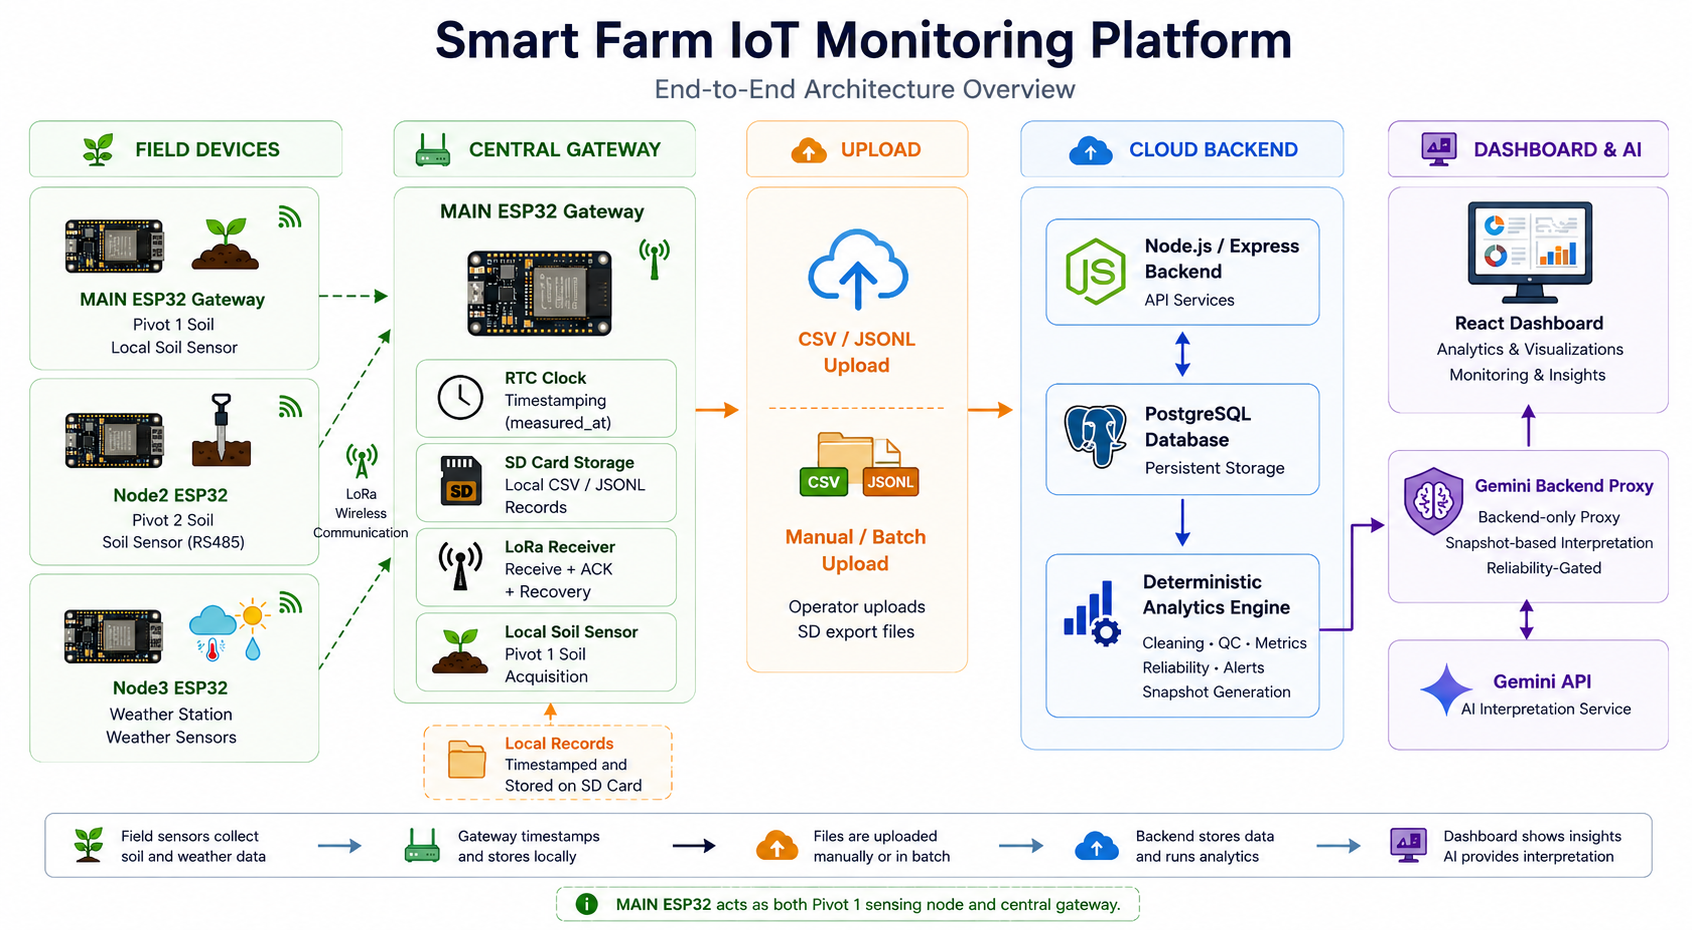
\includegraphics[width=\textwidth]{figures/overall-diagram}
% TODO: copy Academic-Thesis/Diagrams/overall diagram.png to figures/overall-diagram.png before compiling
\caption{Overall system architecture showing the three hardware nodes, LoRa wireless communication, SD-based local storage, and the cloud backend and dashboard layers.}
\label{fig:overall-system-architecture}
\end{figure}

The MAIN gateway node is the operational centre of the field tier. It coordinates the measurement cycle of all three nodes, maintains the authoritative real-time clock, manages SD card storage, and orchestrates data upload. Node2, a remote soil sensing unit deployed at the second irrigation pivot, acquires soil measurements and transmits them to MAIN via LoRa. Node3, a dedicated weather node, collects atmospheric parameters and transmits them independently over the same LoRa link. The three nodes operate within a structured superframe of ten-minute duration, during which each node executes its sensing task, transmits its packet, and returns to a low-power state.

When an Internet connection is made available, the operator activates Upload Mode by holding the MAIN gateway button. Stored SD records are transmitted in batch to the WebService backend, where they are ingested into a PostgreSQL database. The upload process preserves the RTC-derived measurement timestamp for every reading; the upload timestamp is stored separately as transfer audit metadata and is never used in place of the measurement time for any analytical purpose. This distinction, identified as a gap in related works reviewed in Chapter~\ref{chap:related-works}, is enforced at every layer of the implementation.

\begin{figure}[H]
\centering
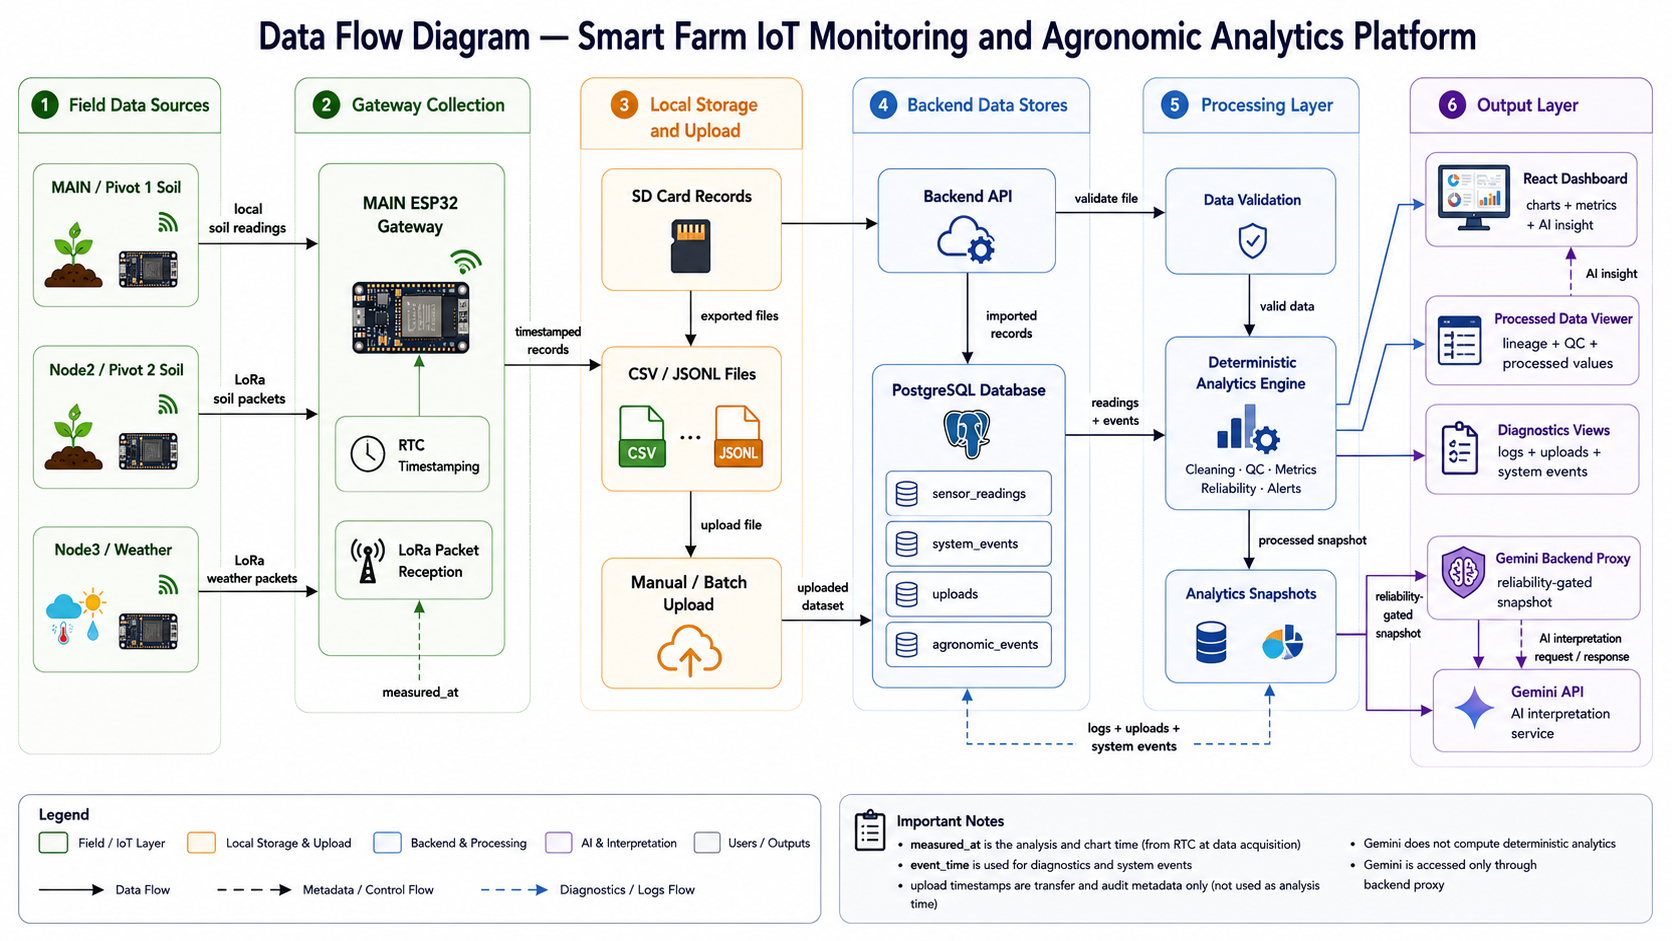
\includegraphics[width=\textwidth]{figures/data-flow-diagram}
% TODO: copy Academic-Thesis/Diagrams/Data Flow Diagram.png to figures/data-flow-diagram.png before compiling
\caption{Data flow diagram illustrating the movement of sensor readings from field acquisition through local storage, batch upload, backend ingestion, and dashboard presentation.}
\label{fig:data-flow-diagram}
\end{figure}

Figure~\ref{fig:data-flow-diagram} traces the complete data path from sensor to dashboard. All measurement data flows from sensors through the MAIN gateway, where it is timestamped and stored locally. Upload transfers SD content to the backend; the backend performs ingestion, validation, and analytics snapshot computation. The dashboard retrieves data through the backend API and presents readings, events, diagnostics, and analytics to the operator. At no stage in this flow does the upload timestamp overwrite or substitute for the RTC-derived measurement timestamp.

% ============================================================
\section{Hardware Architecture}
\label{sec:hardware}
% ============================================================

The system is composed of three hardware nodes, each serving a distinct role in the field monitoring architecture. Table~\ref{tab:node-roles} summarises the roles and primary responsibilities of each node.

\begin{table}[H]
\centering
\caption{Summary of node roles in the system architecture.}
\label{tab:node-roles}
\small
\begin{tabular}{p{2.5cm} p{3.0cm} p{4.0cm} p{4.5cm}}
\hline
\textbf{Node} & \textbf{Microcontroller} & \textbf{Primary function} & \textbf{Location} \\
\hline
MAIN gateway & ESP32 38-pin & Coordination, Pivot~1 soil sensing, RTC, SD storage, upload & Field base station (Pivot~1 location) \\
\hline
Node2 & ESP32-C3 Super Mini & Pivot~2 soil sensing, LoRa transmission & Pivot~2 location (remote) \\
\hline
Node3 & ESP32-C3 Super Mini & Weather monitoring, LoRa transmission & Field weather station position \\
\hline
\end{tabular}
\end{table}

% ----------------------------------------------------------
\subsection{MAIN ESP32 Gateway Node}
\label{sec:main-node}
% ----------------------------------------------------------

The MAIN node is an ESP32 38-pin development board that serves as the operational centre of the field sensing network. It performs four distinct functions within each measurement cycle: it opens a LoRa receive window to collect packets from Node2 and Node3, it reads the local soil sensor at Pivot~1 via RS485/Modbus, it writes all acquired readings and events to the SD card, and it manages upload and RTC synchronisation when requested by the operator.

\begin{figure}[H]
\centering
\begin{minipage}[b]{0.48\textwidth}
\centering
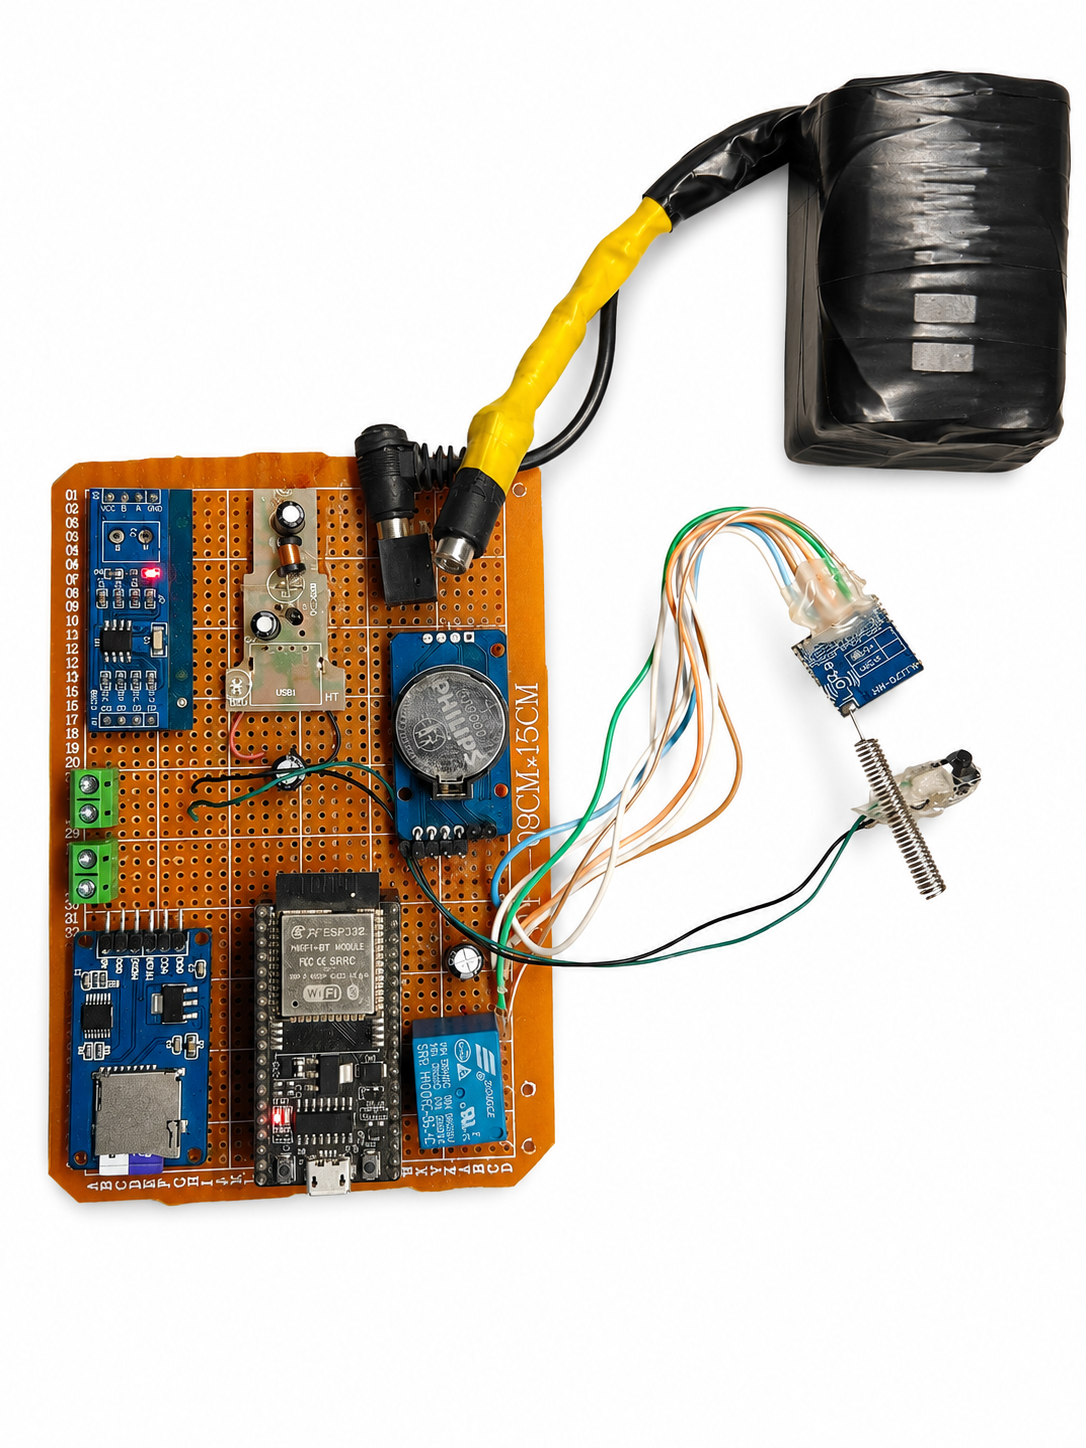
\includegraphics[width=\textwidth]{figures/MainNodeFront}
% TODO: copy Academic-Thesis/SystemImage/MainNodeFront.png to figures/MainNodeFront.png before compiling
\caption{MAIN gateway node — front view showing the ESP32 board, RTC module, and LoRa transceiver.}
\label{fig:main-node-front}
\end{minipage}
\hfill
\begin{minipage}[b]{0.48\textwidth}
\centering
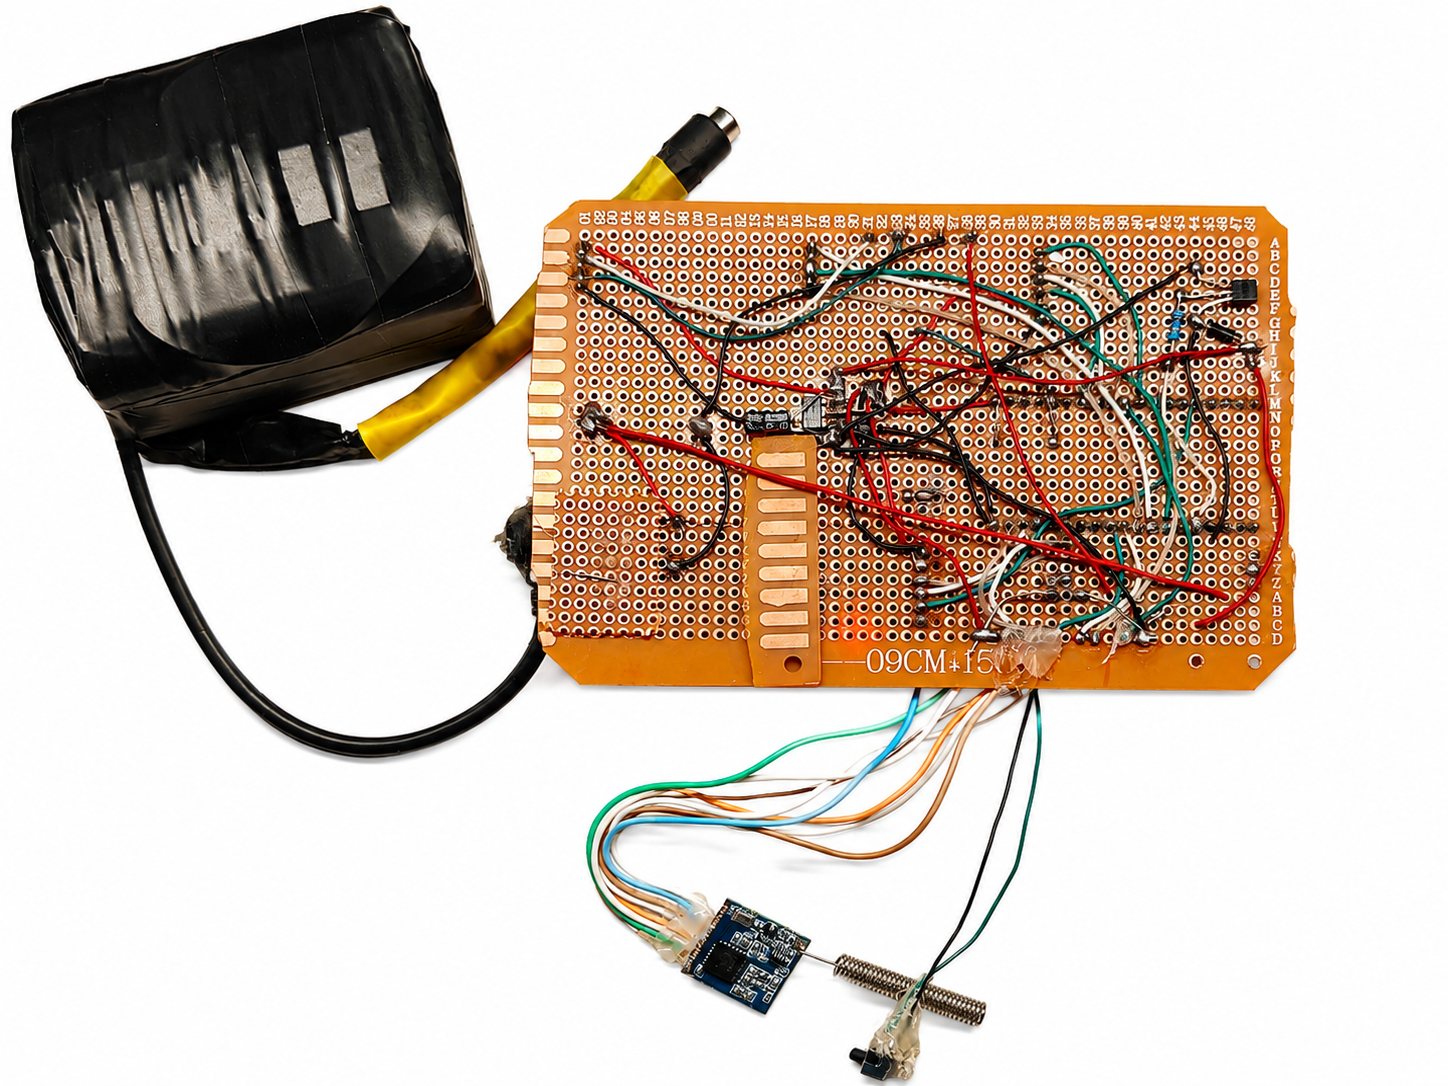
\includegraphics[width=\textwidth]{figures/MainNodeBack}
% TODO: copy Academic-Thesis/SystemImage/MainNodeBack.png to figures/MainNodeBack.png before compiling
\caption{MAIN gateway node — rear view showing the SD card module and wiring connections.}
\label{fig:main-node-back}
\end{minipage}
\end{figure}

\begin{figure}[H]
\centering
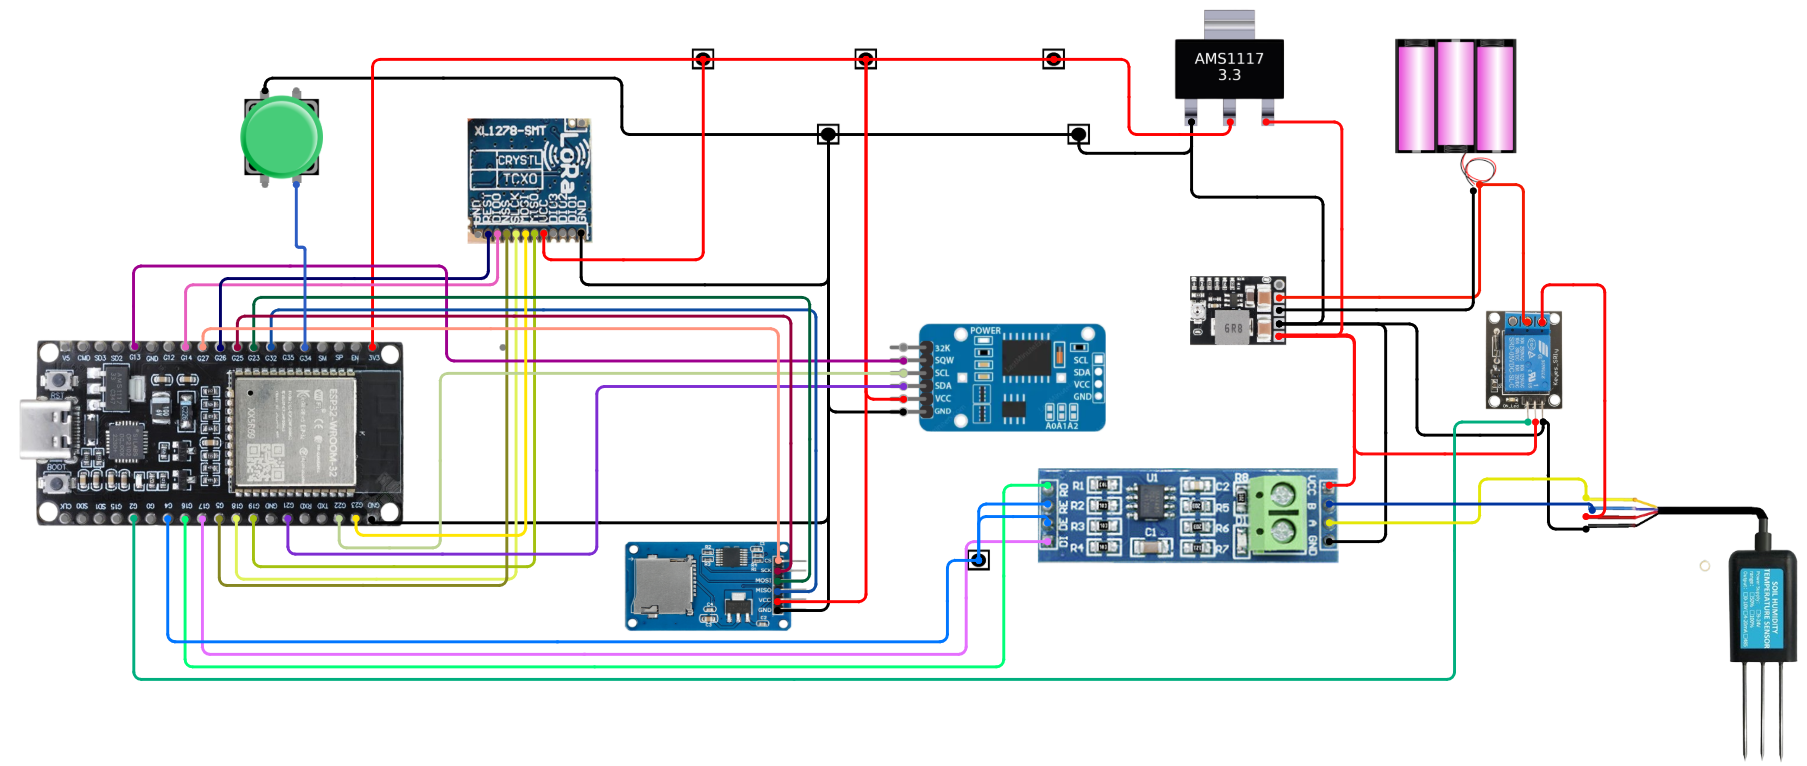
\includegraphics[width=0.85\textwidth]{figures/MainNodeWiringDiagram}
% TODO: copy Academic-Thesis/Diagrams/MainNodeWiringDiagram.png to figures/MainNodeWiringDiagram.png before compiling
\caption{MAIN gateway node wiring diagram showing pin connections between the ESP32, DS3231 RTC, SD card module, SX127x LoRa transceiver, MAX485 RS485 interface, and relay module.}
\label{fig:main-node-wiring}
\end{figure}

The MAIN node integrates five hardware subsystems. The DS3231 RTC module, connected over I2C (SDA\,=\,GPIO21, SCL\,=\,GPIO22), provides the authoritative measurement timestamp. A dedicated SPI bus (VSPI: MISO\,=\,GPIO19, MOSI\,=\,GPIO23, SCK\,=\,GPIO18, CS\,=\,GPIO5, RST\,=\,GPIO26, DIO0\,=\,GPIO14) connects the SX127x LoRa transceiver for wireless reception from remote nodes. A second SPI bus (HSPI: MISO\,=\,GPIO32, MOSI\,=\,GPIO33, SCK\,=\,GPIO25, CS\,=\,GPIO27) connects the SD card module for local data persistence. A MAX485 RS485 transceiver and relay module serve the local Pivot~1 soil sensor; the relay is used to control sensor power and is switched on immediately before a measurement and switched off immediately after, regardless of whether the read succeeds.

\begin{figure}[H]
\centering
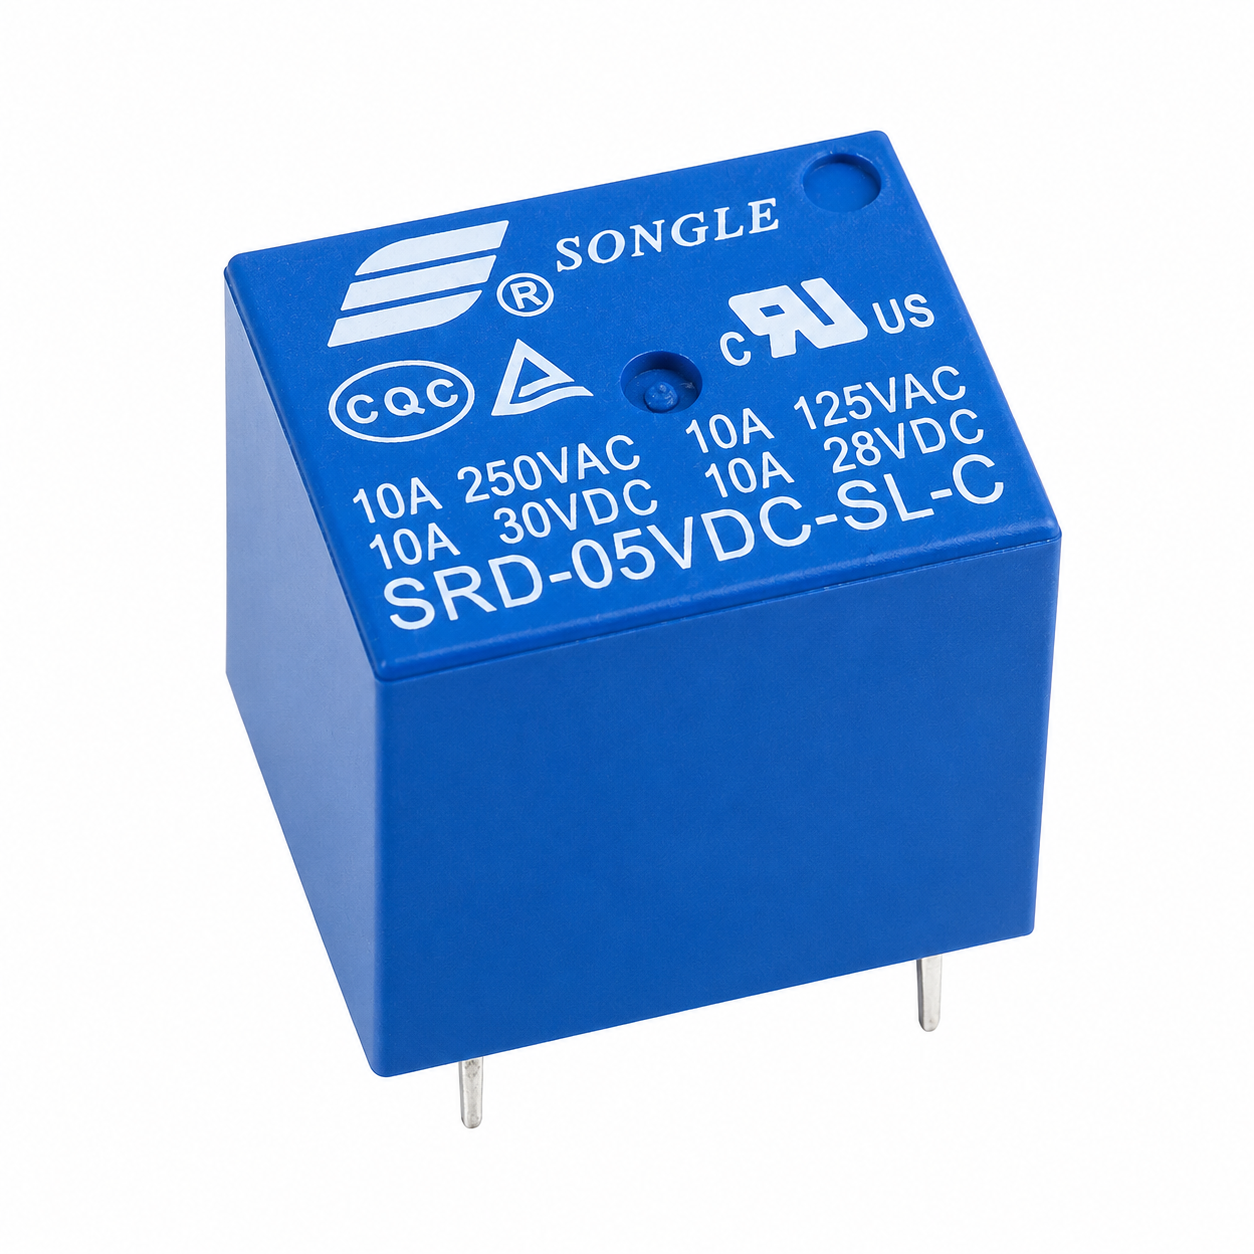
\includegraphics[width=0.35\textwidth]{figures/Relay}
% TODO: copy Academic-Thesis/SystemImage/Relay.png to figures/Relay.png before compiling
\caption{Relay module used on the MAIN node and Node2 to control RS485 soil sensor power. The relay is activated for the duration of the sensor warmup and read sequence and deactivated immediately after to minimise continuous current draw.}
\label{fig:relay-module-ch3}
\end{figure}

The Pivot~1 local soil sensor is interfaced over RS485 using Modbus RTU at 4800~baud, 8N1, with slave address 0x01, function code 0x03, and three registers beginning at address 0x0000, yielding soil moisture (tenths of a percent), soil temperature (tenths of a degree Celsius), and soil EC (integer, µS/cm). The firmware activates the relay, waits 15~seconds for sensor warm-up, issues the Modbus query, then deactivates the relay. During the validation period documented in Part~B, the Modbus register map for the Pivot~1 sensor was not yet finalised in the firmware; the \texttt{performLocalSoilMeasurement()} routine completes the relay control sequence on each cycle, but the register read returns a \texttt{LOCAL\_SOIL\_REGISTER\_MAP\_MISSING} diagnostic code rather than measured values. This state is reflected accurately in the validation evidence. The Pivot~1 hardware path is fully wired and the firmware structure is in place; the register map will be confirmed when the sensor's Modbus documentation is verified against the installed unit.

A push-button on GPIO34 provides the operator interface for Upload Mode and RTC Synchronisation Mode. A long press (sustained contact of one second or more) triggers batch upload of SD content. Four consecutive short presses trigger RTC synchronisation. The MAIN node does not expose a network interface during normal sensing cycles; network activity occurs only during Upload Mode.

% ----------------------------------------------------------
\subsection{Node2 Remote Soil Node}
\label{sec:node2}
% ----------------------------------------------------------

Node2 is an ESP32-C3 Super Mini development board deployed at the Pivot~2 location, physically separated from the MAIN gateway. Its sole sensing responsibility is the acquisition of soil moisture, temperature, and EC from the soil sensor installed at Pivot~2. Because Pivot~1 and Pivot~2 represent distinct irrigation zones with independent soil conditions, the two soil data streams are complementary rather than redundant.

\begin{figure}[H]
\centering
\begin{minipage}[b]{0.48\textwidth}
\centering
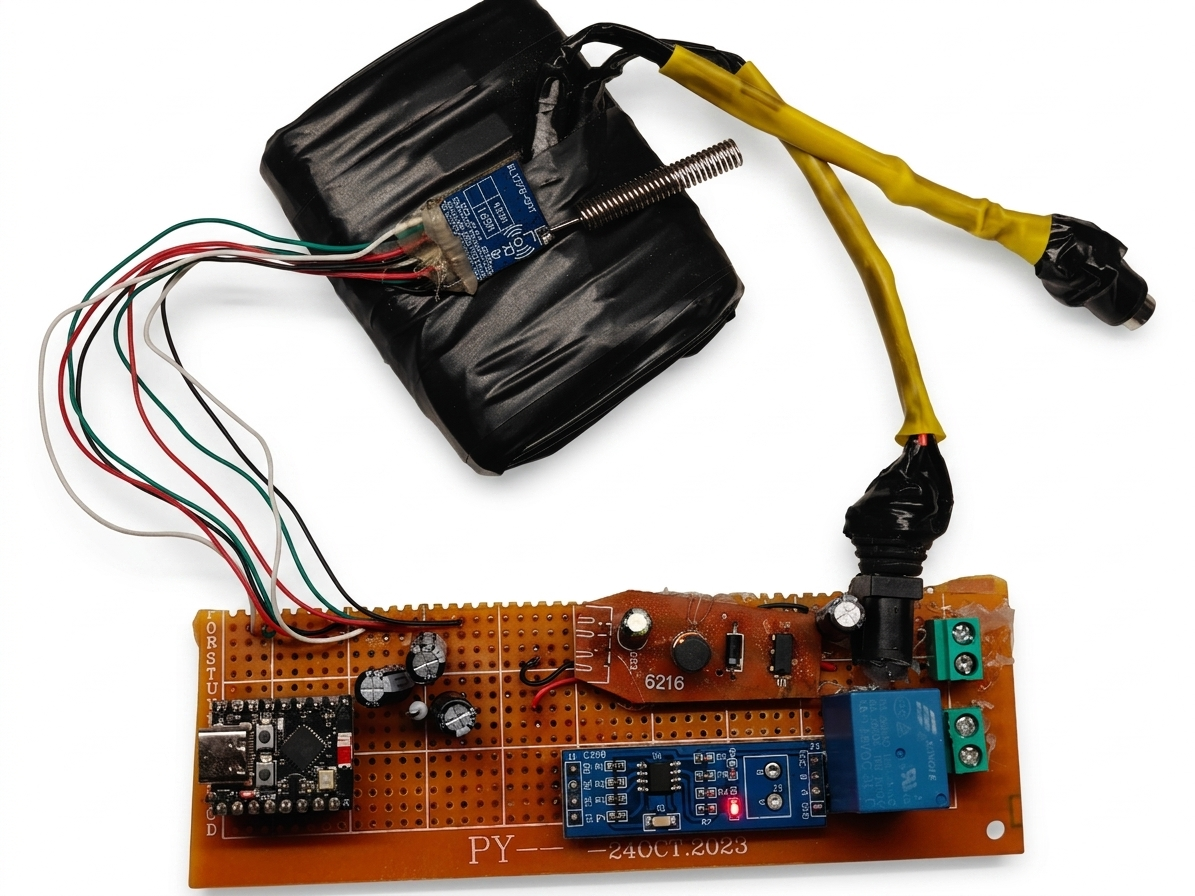
\includegraphics[width=\textwidth]{figures/SecondNodeFront}
% TODO: copy Academic-Thesis/SystemImage/SecondNodeFront.png to figures/SecondNodeFront.png before compiling
\caption{Node2 soil node — front view showing the ESP32-C3 board and LoRa module.}
\label{fig:node2-front}
\end{minipage}
\hfill
\begin{minipage}[b]{0.48\textwidth}
\centering
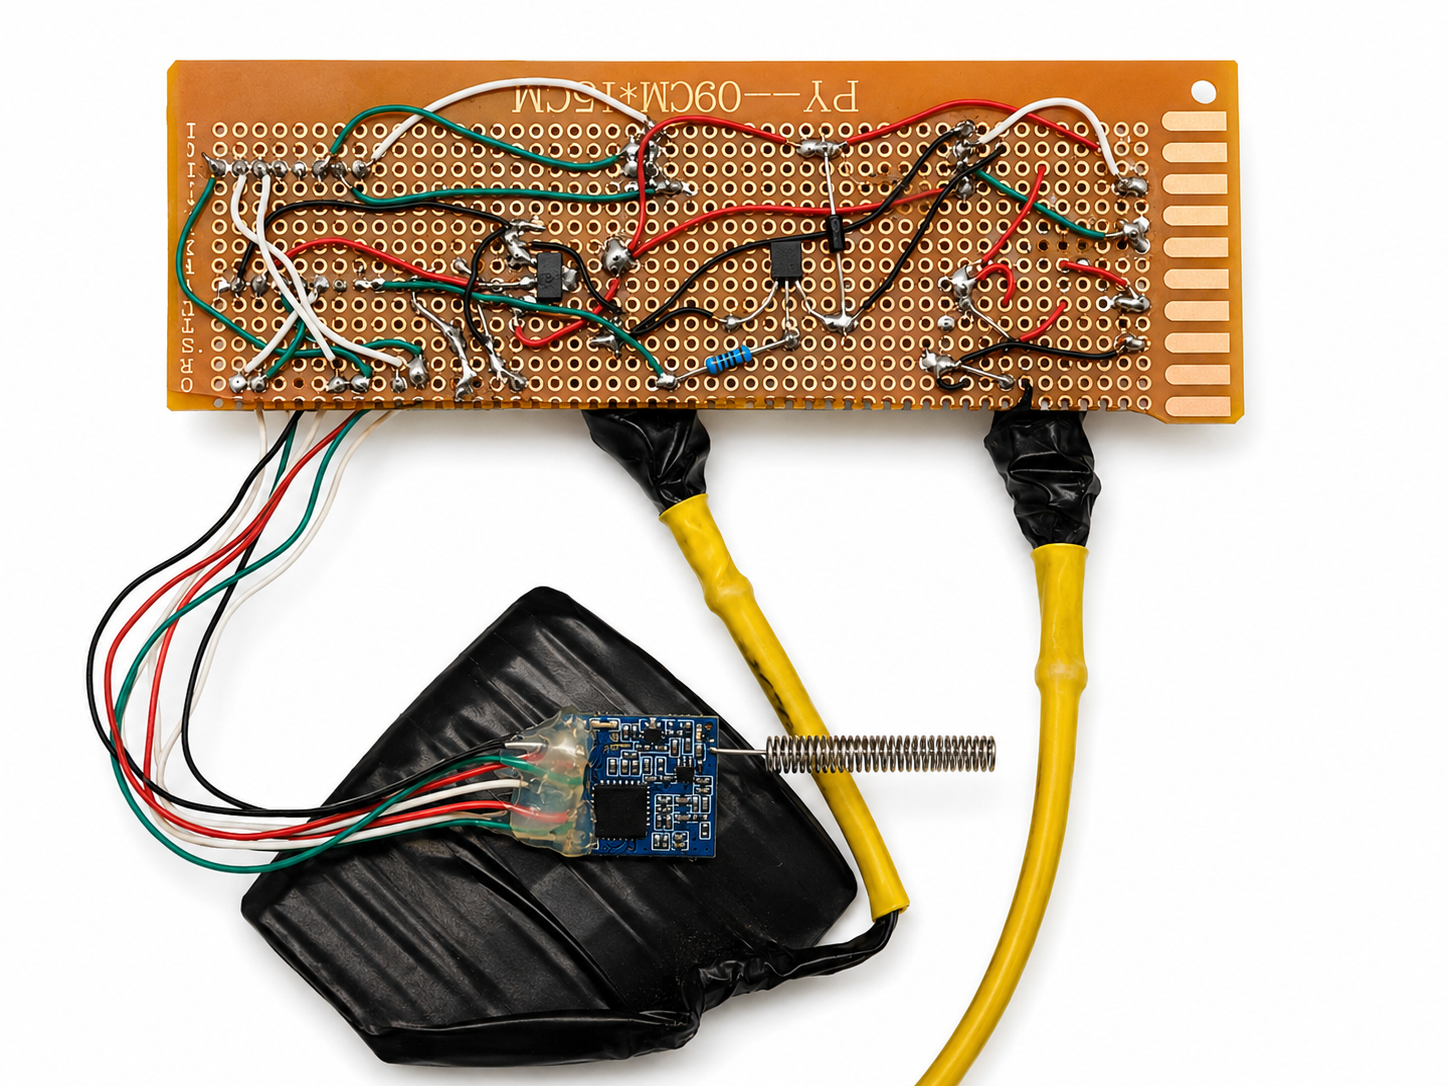
\includegraphics[width=\textwidth]{figures/SecondNodeBack}
% TODO: copy Academic-Thesis/SystemImage/SecondNodeBack.png to figures/SecondNodeBack.png before compiling
\caption{Node2 soil node — rear view showing the MAX485 interface and relay wiring.}
\label{fig:node2-back}
\end{minipage}
\end{figure}

\begin{figure}[H]
\centering
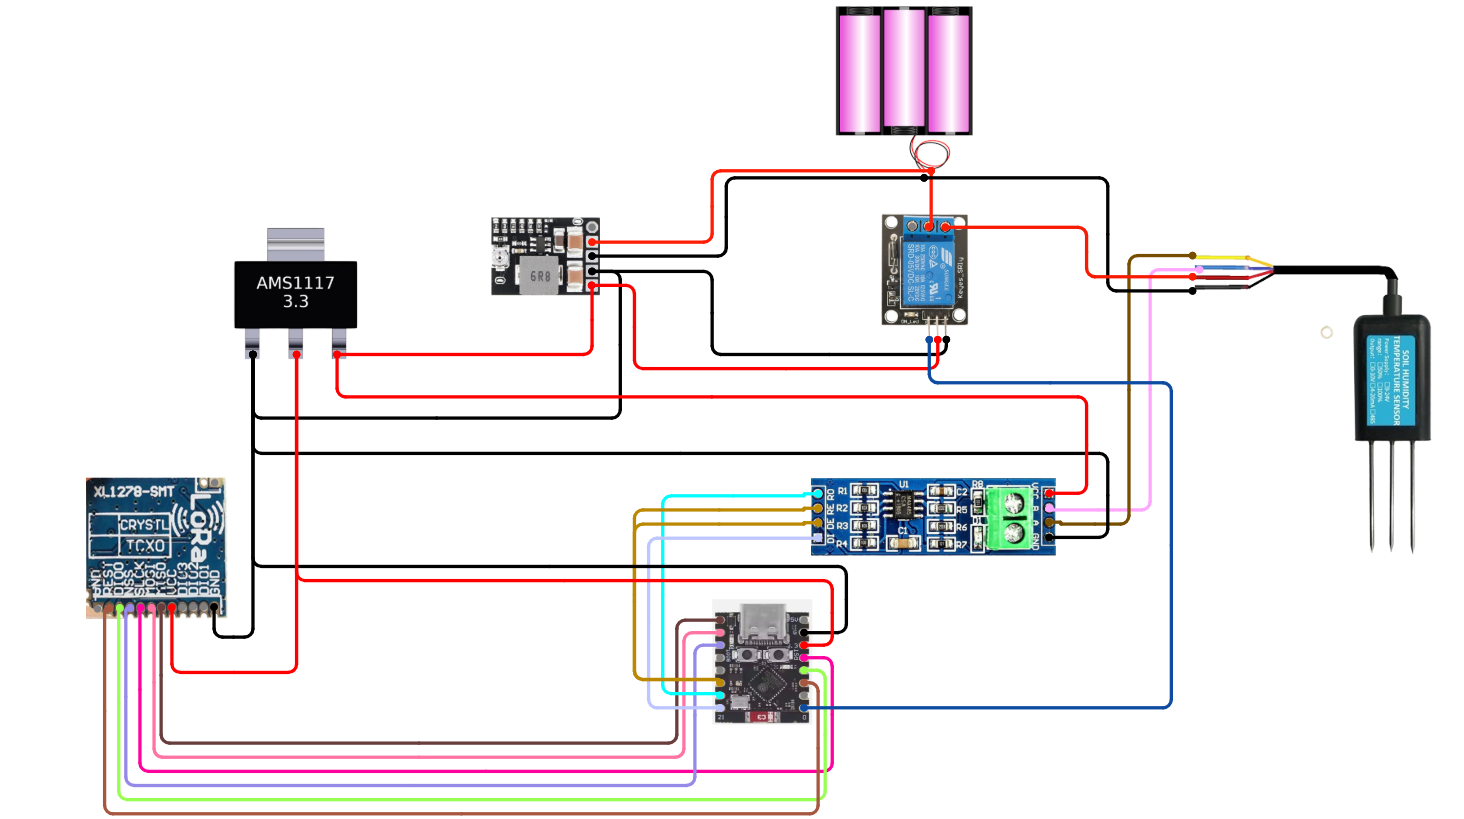
\includegraphics[width=0.85\textwidth]{figures/Node2WiringDiagram}
% TODO: copy Academic-Thesis/Diagrams/Node2WiringDiagram.png to figures/Node2WiringDiagram.png before compiling
\caption{Node2 wiring diagram showing pin connections between the ESP32-C3, SX127x LoRa transceiver, MAX485 RS485 interface, relay module, and RS485 soil sensor.}
\label{fig:node2-wiring}
\end{figure}

The LoRa transceiver is connected to the ESP32-C3 SPI bus (SCK\,=\,GPIO4, MISO\,=\,GPIO5, MOSI\,=\,GPIO6, CS\,=\,GPIO7, RST\,=\,GPIO2, DIO0\,=\,GPIO3). The MAX485 RS485 transceiver uses GPIO10 for the direction control (DE/RE combined), GPIO20 for the receive line (RO), and GPIO21 for the transmit line (DI). A relay on GPIO0 controls power to the RS485 soil sensor, applying the same relay-on, warm-up, read, relay-off sequence used on the MAIN node.

\begin{figure}[H]
\centering
\begin{minipage}[b]{0.45\textwidth}
\centering
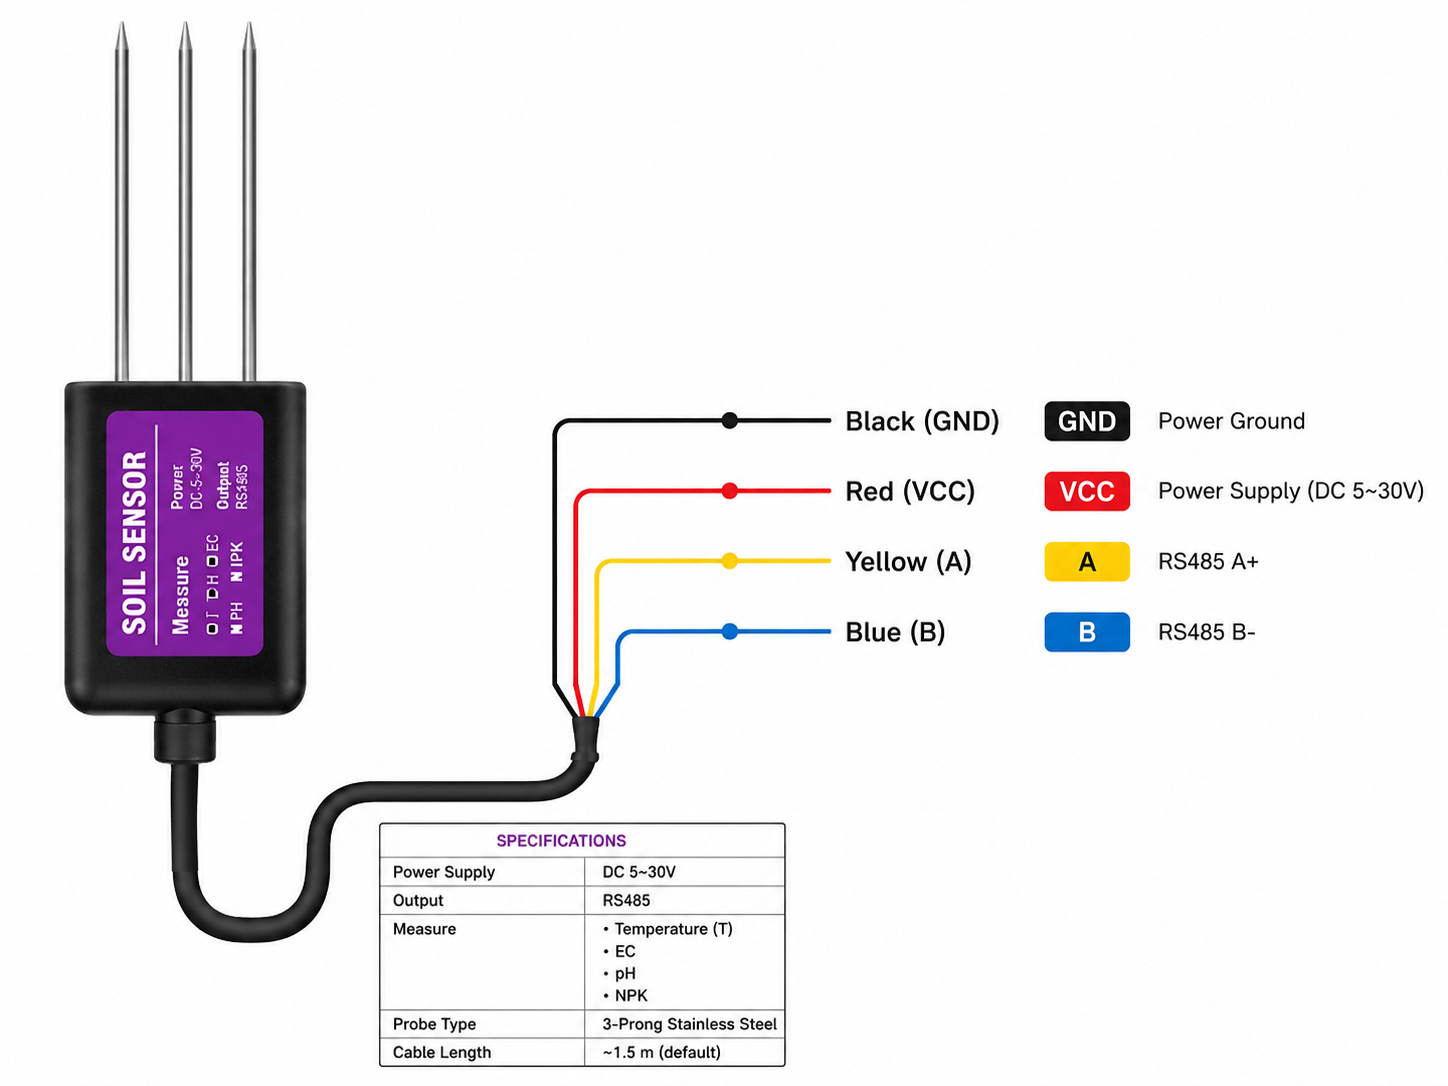
\includegraphics[width=\textwidth]{figures/SoilSensor}
% TODO: copy Academic-Thesis/SystemImage/SoilSensor.png to figures/SoilSensor.png before compiling
\caption{RS485 soil sensor measuring moisture, temperature, and EC. The sensor is shared in design between the MAIN local (Pivot~1) and Node2 remote (Pivot~2) installations.}
\label{fig:soil-sensor}
\end{minipage}
\hfill
\begin{minipage}[b]{0.45\textwidth}
\centering
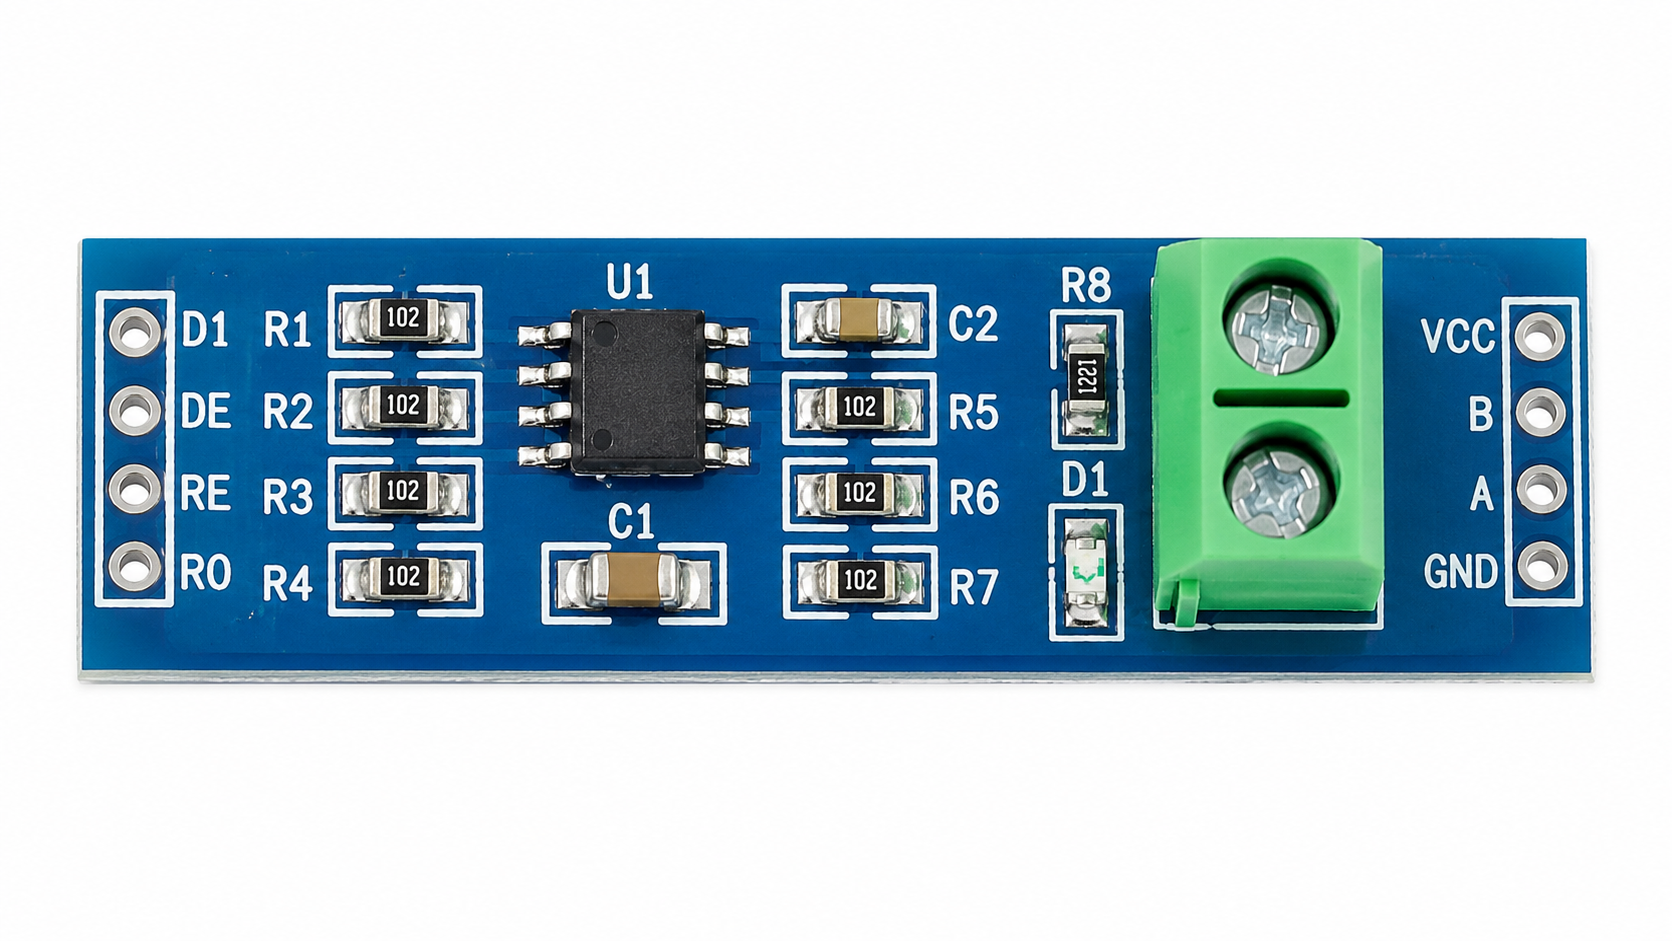
\includegraphics[width=\textwidth]{figures/Max485}
% TODO: copy Academic-Thesis/SystemImage/Max485.png to figures/Max485.png before compiling
\caption{MAX485 RS485 transceiver module used on both the MAIN node and Node2 for half-duplex serial communication with the Modbus soil sensor.}
\label{fig:max485}
\end{minipage}
\end{figure}

After completing its measurement, Node2 encodes the three sensor values into a LoRa packet and transmits at 433~MHz, spreading factor SF7, bandwidth 125~kHz, coding rate 4/5, with CRC enabled and a transmit power of 14~dBm. Node2 then enters deep sleep, with an interrupt scheduled to fire at the next transmission slot within the ten-minute superframe. The deep sleep interval is the primary mechanism by which Node2 conserves battery energy between measurement cycles.

% ----------------------------------------------------------
\subsection{Node3 Weather Node}
\label{sec:node3}
% ----------------------------------------------------------

Node3 is a second ESP32-C3 Super Mini, deployed as a dedicated atmospheric monitoring station. It measures air temperature, relative humidity, and barometric pressure using a BME280 sensor connected over I2C (SDA\,=\,GPIO8, SCL\,=\,GPIO9). The LoRa transceiver uses the same SPI pin assignment as Node2 (SCK\,=\,GPIO4, MISO\,=\,GPIO5, MOSI\,=\,GPIO6, CS\,=\,GPIO7, RST\,=\,GPIO2, DIO0\,=\,GPIO3).

\begin{figure}[H]
\centering
\begin{minipage}[b]{0.48\textwidth}
\centering
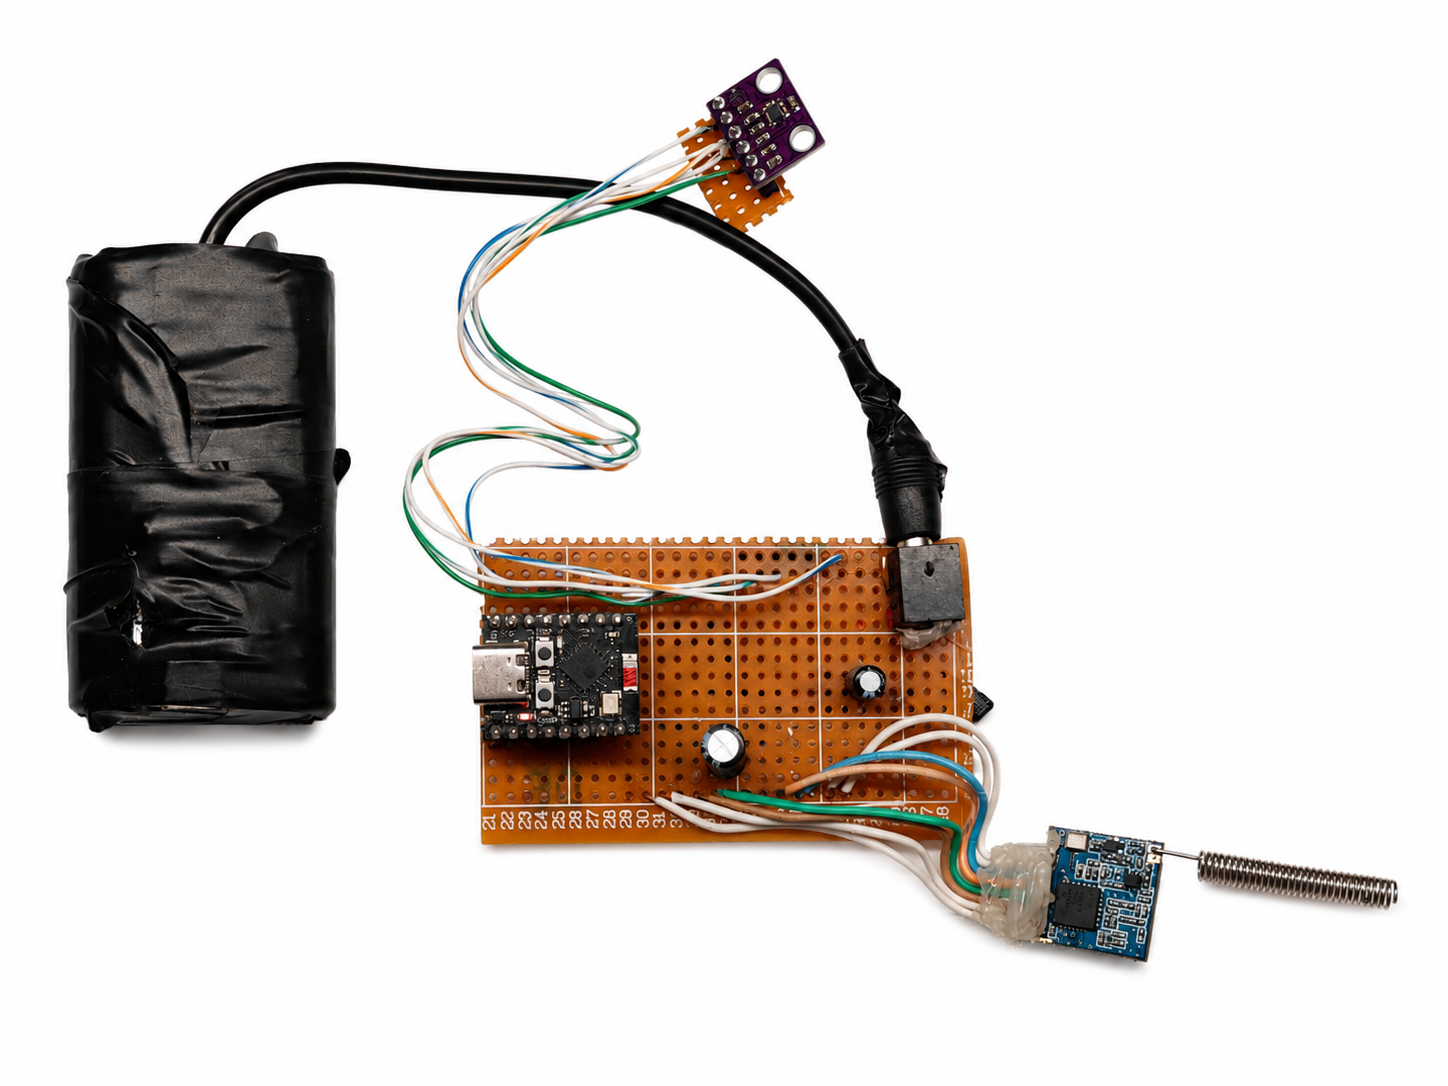
\includegraphics[width=\textwidth]{figures/WatherNodeFront}
% TODO: rename WatherNodeFront.png to WeatherNodeFront.png in Academic-Thesis/SystemImage/ for consistency; copy to figures/WatherNodeFront.png before compiling
\caption{Node3 weather node — front view showing the ESP32-C3 board, BME280 sensor, and LoRa module.}
\label{fig:node3-front}
\end{minipage}
\hfill
\begin{minipage}[b]{0.48\textwidth}
\centering
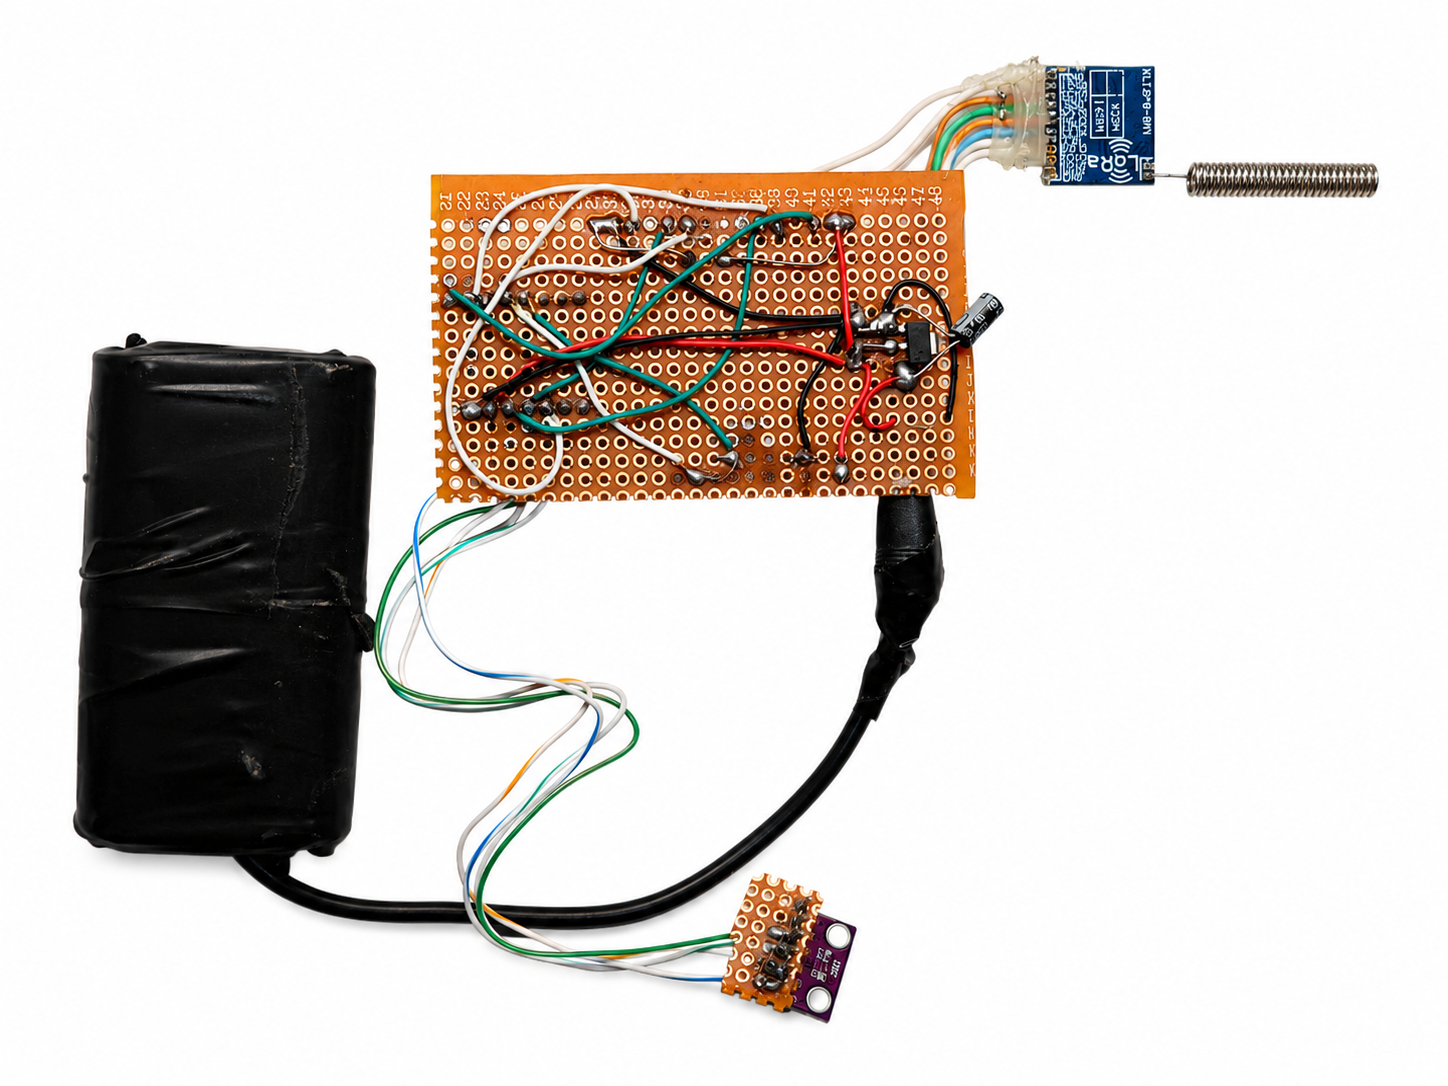
\includegraphics[width=\textwidth]{figures/WatherNodeBack}
% TODO: rename WatherNodeBack.png to WeatherNodeBack.png in Academic-Thesis/SystemImage/ for consistency; copy to figures/WatherNodeBack.png before compiling
\caption{Node3 weather node — rear view showing the I2C connections to the BME280 module.}
\label{fig:node3-back}
\end{minipage}
\end{figure}

\begin{figure}[H]
\centering
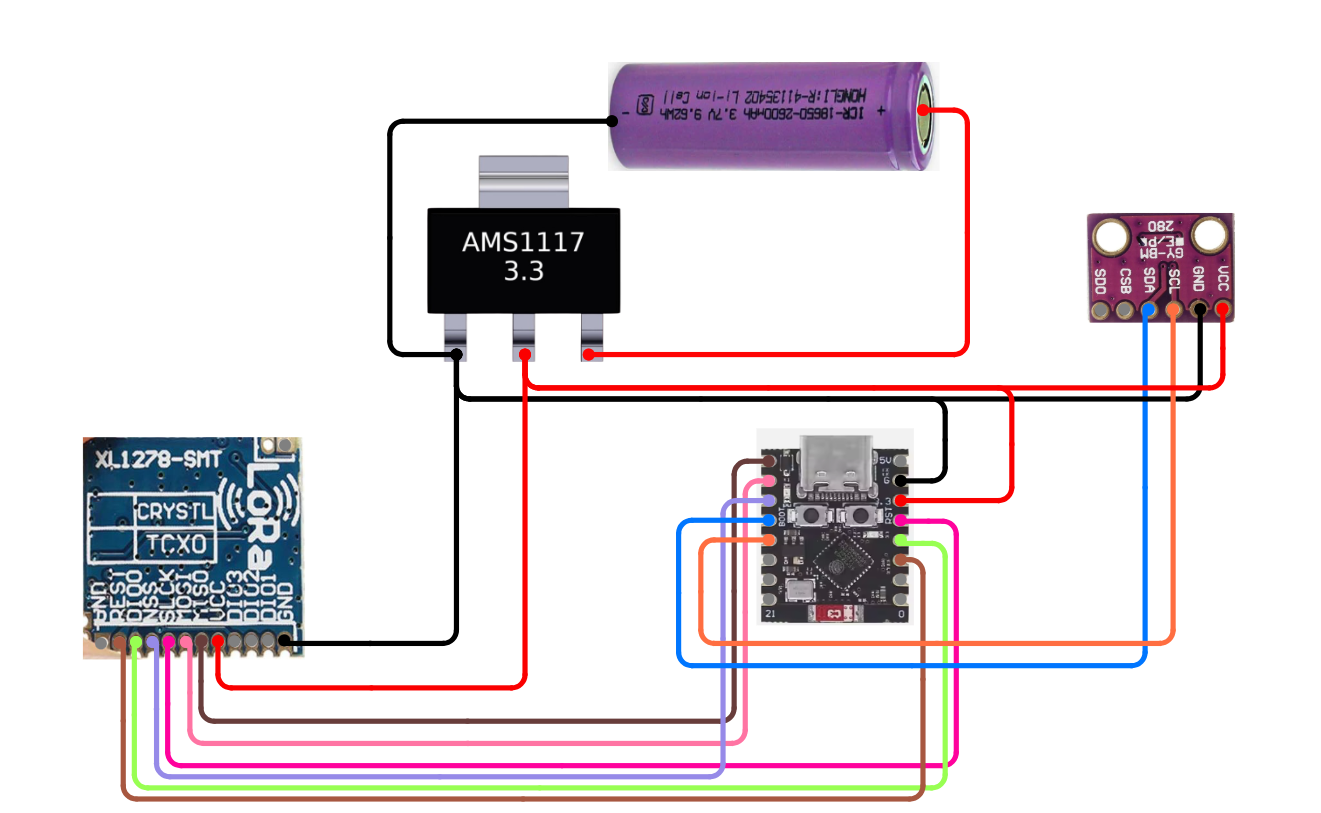
\includegraphics[width=0.85\textwidth]{figures/WatherNodeWiringDiagram}
% TODO: rename WatherNodeWiringDiagram.png to WeatherNodeWiringDiagram.png in Academic-Thesis/Diagrams/ for consistency; copy to figures/WatherNodeWiringDiagram.png before compiling
\caption{Node3 weather node wiring diagram showing connections between the ESP32-C3, BME280 environmental sensor (I2C), and SX127x LoRa transceiver (SPI).}
\label{fig:node3-wiring}
\end{figure}

The BME280 is operated in forced measurement mode, a single-shot acquisition pattern in which the sensor is commanded to take one reading, delivers the result, and returns to sleep mode automatically. This eliminates the continuous power draw that would result from leaving the sensor in normal (continuous) mode. The active measurement window per cycle is under two seconds, after which Node3 encodes its three atmospheric values, transmits the LoRa packet, and returns to deep sleep. No relay is required for Node3 because the BME280's own forced-mode power management is sufficient.

\begin{figure}[H]
\centering
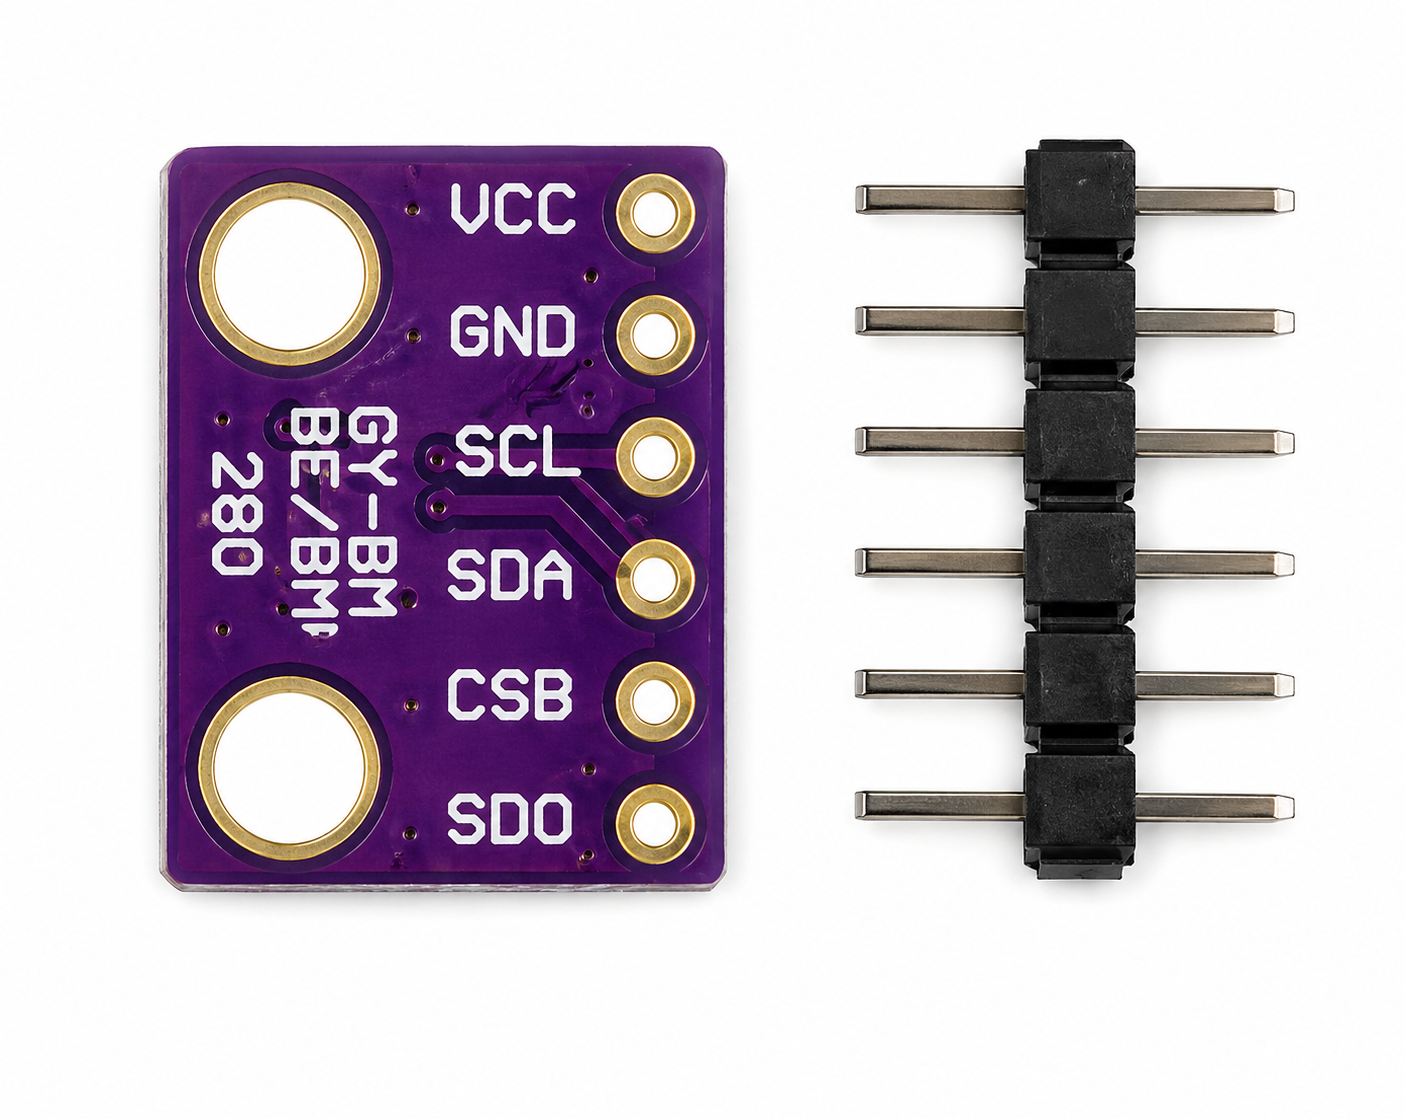
\includegraphics[width=0.35\textwidth]{figures/Bme280}
% TODO: copy Academic-Thesis/SystemImage/Bme280.png to figures/Bme280.png before compiling
\caption{BME280 environmental sensor module measuring air temperature, relative humidity, and barometric pressure. The sensor is operated in forced measurement mode to eliminate continuous current draw between measurement cycles.}
\label{fig:bme280-ch3}
\end{figure}

Table~\ref{tab:hardware-components} provides a consolidated reference of the hardware components used across all three nodes.

\begin{table}[H]
\centering
\caption{Hardware components used across the three system nodes.}
\label{tab:hardware-components}
\small
\begin{tabular}{p{3.5cm} p{2.5cm} p{3.5cm} p{4.5cm}}
\hline
\textbf{Component} & \textbf{Node(s)} & \textbf{Interface} & \textbf{Function} \\
\hline
ESP32 38-pin & MAIN & — & Gateway microcontroller; host for all subsystems \\
\hline
ESP32-C3 Super Mini & Node2, Node3 & — & Remote node microcontroller \\
\hline
SX127x LoRa module & All & SPI & 433~MHz long-range wireless communication \\
\hline
DS3231 RTC & MAIN & I2C & Authoritative real-time clock; \texttt{measured\_at} source \\
\hline
SD card module & MAIN & SPI & Local storage of readings and events in CSV/JSONL \\
\hline
MAX485 RS485 & MAIN, Node2 & UART & Half-duplex Modbus RTU interface to soil sensor \\
\hline
RS485 soil sensor & MAIN (Pivot~1), Node2 (Pivot~2) & RS485 & Soil moisture~(\%), temperature~(°C), EC~(µS/cm) \\
\hline
Relay module & MAIN, Node2 & GPIO & Sensor power control; eliminates standby current draw \\
\hline
BME280 & Node3 & I2C & Air temperature, humidity, barometric pressure \\
\hline
Push-button & MAIN & GPIO34 & Upload Mode and RTC Synchronisation trigger \\
\hline
\end{tabular}
\end{table}

% ============================================================
\section{Firmware Operating Modes: Motivation and Design}
\label{sec:firmware}
% ============================================================

The firmware architecture is structured around eight distinct operating modes, each introduced to address a specific constraint or failure pattern observed during field prototype testing. The modes are not alternative operating states that exclude one another; several activate and deactivate within a single ten-minute cycle. The state machine governing transitions between modes is illustrated in Figure~\ref{fig:firmware-state-machine}.

\begin{figure}[H]
\centering
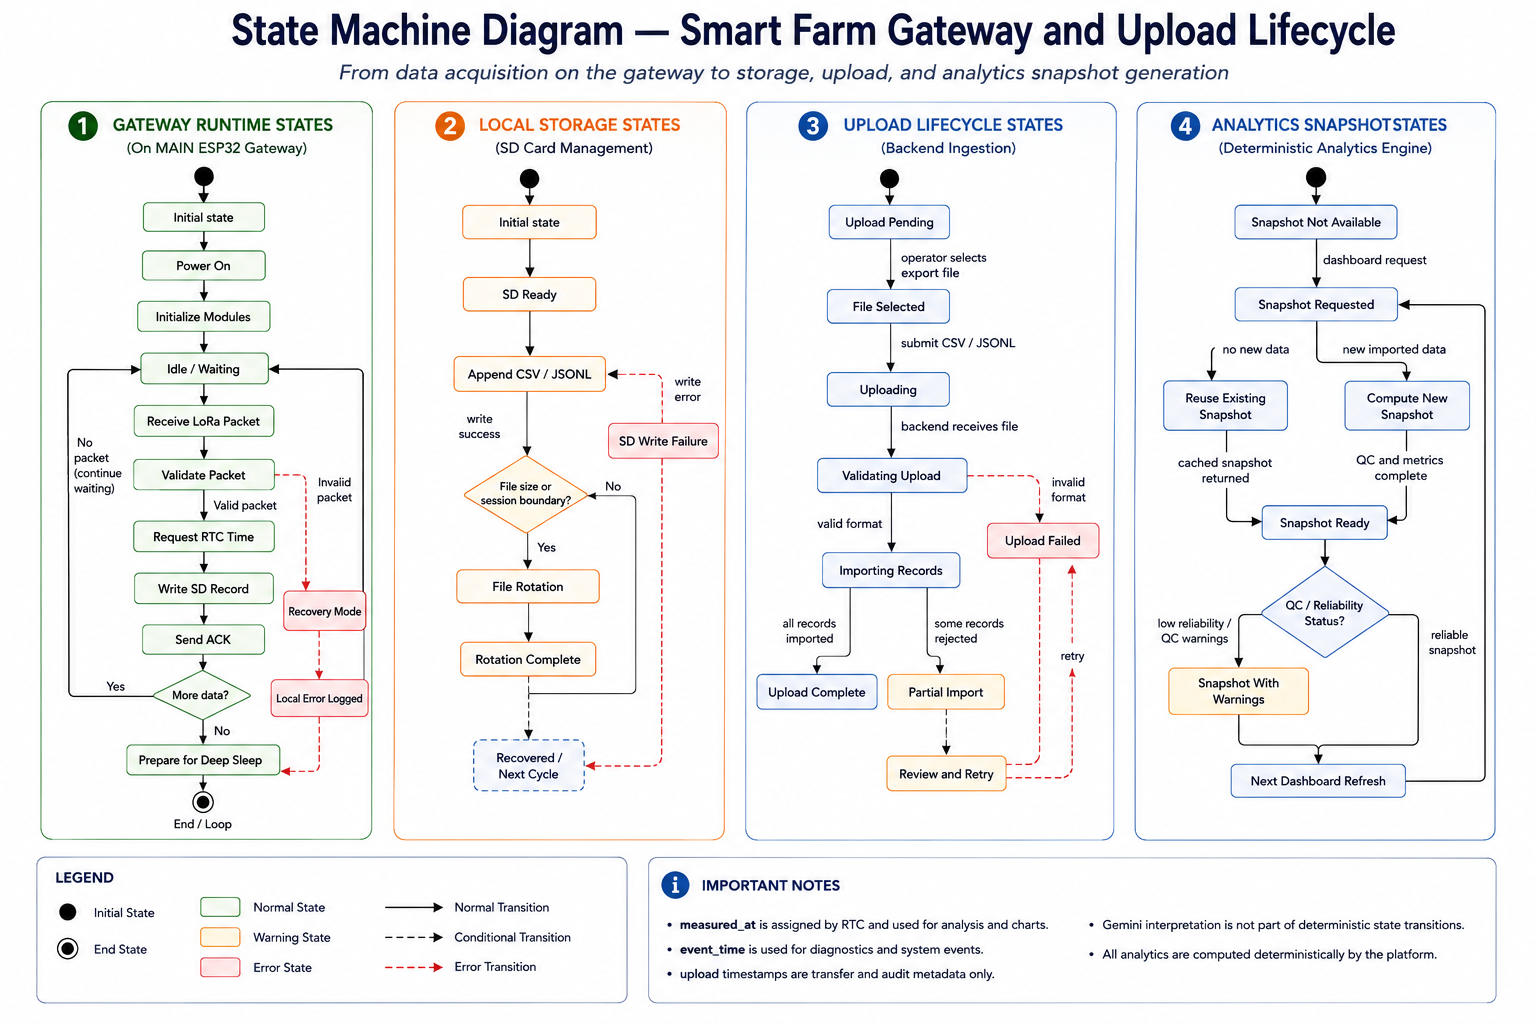
\includegraphics[width=0.85\textwidth]{figures/StateMachineDiagram}
% TODO: copy Academic-Thesis/Diagrams/State Machine Diagram.png to figures/StateMachineDiagram.png before compiling
\caption{Firmware state machine diagram showing the operating modes of the MAIN gateway node, their trigger conditions, and the transitions between them during normal operation, recovery, upload, and RTC synchronisation sequences.}
\label{fig:firmware-state-machine}
\end{figure}

% ----------------------------------------------------------
\subsection{Normal Sensing Mode}
\label{sec:mode-normal}
% ----------------------------------------------------------

Normal Sensing Mode is the default operating state, activated at the start of each ten-minute superframe. During this mode, the MAIN node opens its LoRa receive window to collect packets from Node2 and Node3, performs the Pivot~1 local soil reading, and writes all acquired data to the SD card before entering deep sleep.

The mode is not an always-on polling loop. Rather, it follows a scheduled sequence derived from the superframe timing. Node2 wakes at frame onset, powers its relay, performs its measurement, and transmits within the first 30~seconds of the frame. Node3 wakes independently and transmits shortly after. MAIN's receive window spans 70~seconds from frame start, providing sufficient margin to capture both remote transmissions before executing the local soil read. After SD writing, MAIN sleeps for the remainder of the ten-minute period.

% ----------------------------------------------------------
\subsection{Power Saving Mode}
\label{sec:mode-power-saving}
% ----------------------------------------------------------

Power Saving Mode was introduced in response to a fundamental constraint of the deployment environment: the three nodes are battery-powered, and the agricultural site does not provide stable mains electricity. Continuous sensor polling, continuous radio listening, and always-on sensor power would drain a battery within hours, rendering the system impractical.

The mode operates through four coordinated strategies. Deep sleep is the primary mechanism: the ESP32 and ESP32-C3 microcontrollers are placed in their lowest-power sleep state between measurement windows, with a timer interrupt as the sole wake source. Sensor power is controlled by the relay module; the relay is activated only for the warm-up and read interval and deactivated immediately after, preventing the RS485 soil sensor from drawing current between measurement cycles. The BME280 on Node3 is operated in forced mode, which similarly eliminates continuous sensor power draw. LoRa radio activity is confined to the transmission or reception window within each superframe; the transceiver is not listening or transmitting outside these windows.

Battery autonomy was not formally characterised during the validation window. The Power Saving Mode design is evaluated in qualitative terms: its constituent strategies reduce consumption during the idle intervals that constitute the majority of the ten-minute cycle.

% ----------------------------------------------------------
\subsection{LoRa RX/ACK Mode}
\label{sec:mode-lora-ack}
% ----------------------------------------------------------

During each superframe, the MAIN node operates its LoRa radio in receive mode for a window of 70~seconds. This window accommodates the expected transmission times of Node2 and Node3 with sufficient margin to absorb minor timing drift introduced by deep sleep wake-up jitter.

When a valid packet is received from a remote node, MAIN decodes and validates its contents, stamps the \texttt{measured\_at} field from the DS3231 RTC, writes the reading to the SD queue, and transmits an acknowledgement packet addressed to the source node. The ACK is not a bare confirmation; it carries the current RTC timestamp, which allows remote nodes to detect significant drift in their own sleep timers over extended operation.

The ACK mechanism serves two purposes. First, it confirms to the transmitting node that its packet was received correctly, which informs the node's reliability tracking and prevents redundant retransmission within the same cycle. Second, the ACK timestamp enables passive clock monitoring on remote nodes without requiring a dedicated synchronisation protocol. If a node does not receive an ACK within 1500~milliseconds of its transmission, it records a timeout and applies the Recovery Mode logic described in Section~\ref{sec:mode-recovery}.

% ----------------------------------------------------------
\subsection{Recovery Mode}
\label{sec:mode-recovery}
% ----------------------------------------------------------

Recovery Mode was motivated by a specific failure pattern observed during prototype testing: when a node failed to receive an ACK in one cycle — due to RF interference, timing misalignment, or transient hardware instability — it did not recover autonomously in the following cycle. Instead, the node's deep sleep counter drifted progressively further out of alignment with the MAIN receive window, causing repeated missed cycles until the node was manually power-cycled.

The failure mechanism is a timing mismatch, not merely a packet loss event. A node that sleeps 600~seconds expecting to wake into the MAIN receive window may wake slightly early or late; without ACK feedback, it cannot detect the drift and correct it. Over multiple cycles, small drift values accumulate until the node's transmission falls entirely outside the MAIN receive window.

Recovery Mode addresses this through two coordinated mechanisms. On the node side, an RTC\_DATA\_ATTR counter (\texttt{txFailCount}) persists across deep sleep cycles. Each consecutive ACK failure increments the counter. The node selects its next sleep duration from an adaptive sequence (60~seconds, 120~seconds, 300~seconds, 600~seconds) indexed by \texttt{txFailCount}. This sequence progressively shortens the sleep interval, causing the node to shift its transmission earlier in successive frames until it re-enters the MAIN receive window. On success (ACK received), \texttt{txFailCount} is reset to zero and normal sleep intervals resume.

On the MAIN side, a \texttt{NodeHealth} structure tracks each remote node's \texttt{missedCount} and \texttt{recoveryWatch} state. When a node is missed in a frame, MAIN extends its receive window from 70~seconds to 120~seconds for up to two consecutive frames. This extended window is designed to capture a recovering node whose transmission has shifted earlier than the standard window. If the node is not heard within the extended window over the tolerance period, MAIN logs a \texttt{node\_marked\_dead} event and returns to normal window timing. When the node reappears, a \texttt{node\_back\_online} event is logged and normal tracking resumes.

% ----------------------------------------------------------
\subsection{Local Storage Mode}
\label{sec:mode-storage}
% ----------------------------------------------------------

Local Storage Mode refers to the SD card write sequence that occurs at the end of each sensing cycle, after all LoRa receptions and the local soil read have completed. The MAIN node writes sensor readings to a CSV file and system events to a JSONL file. Both files accumulate across cycles, building an offline record of field conditions that persists independently of network availability.

\begin{figure}[H]
\centering
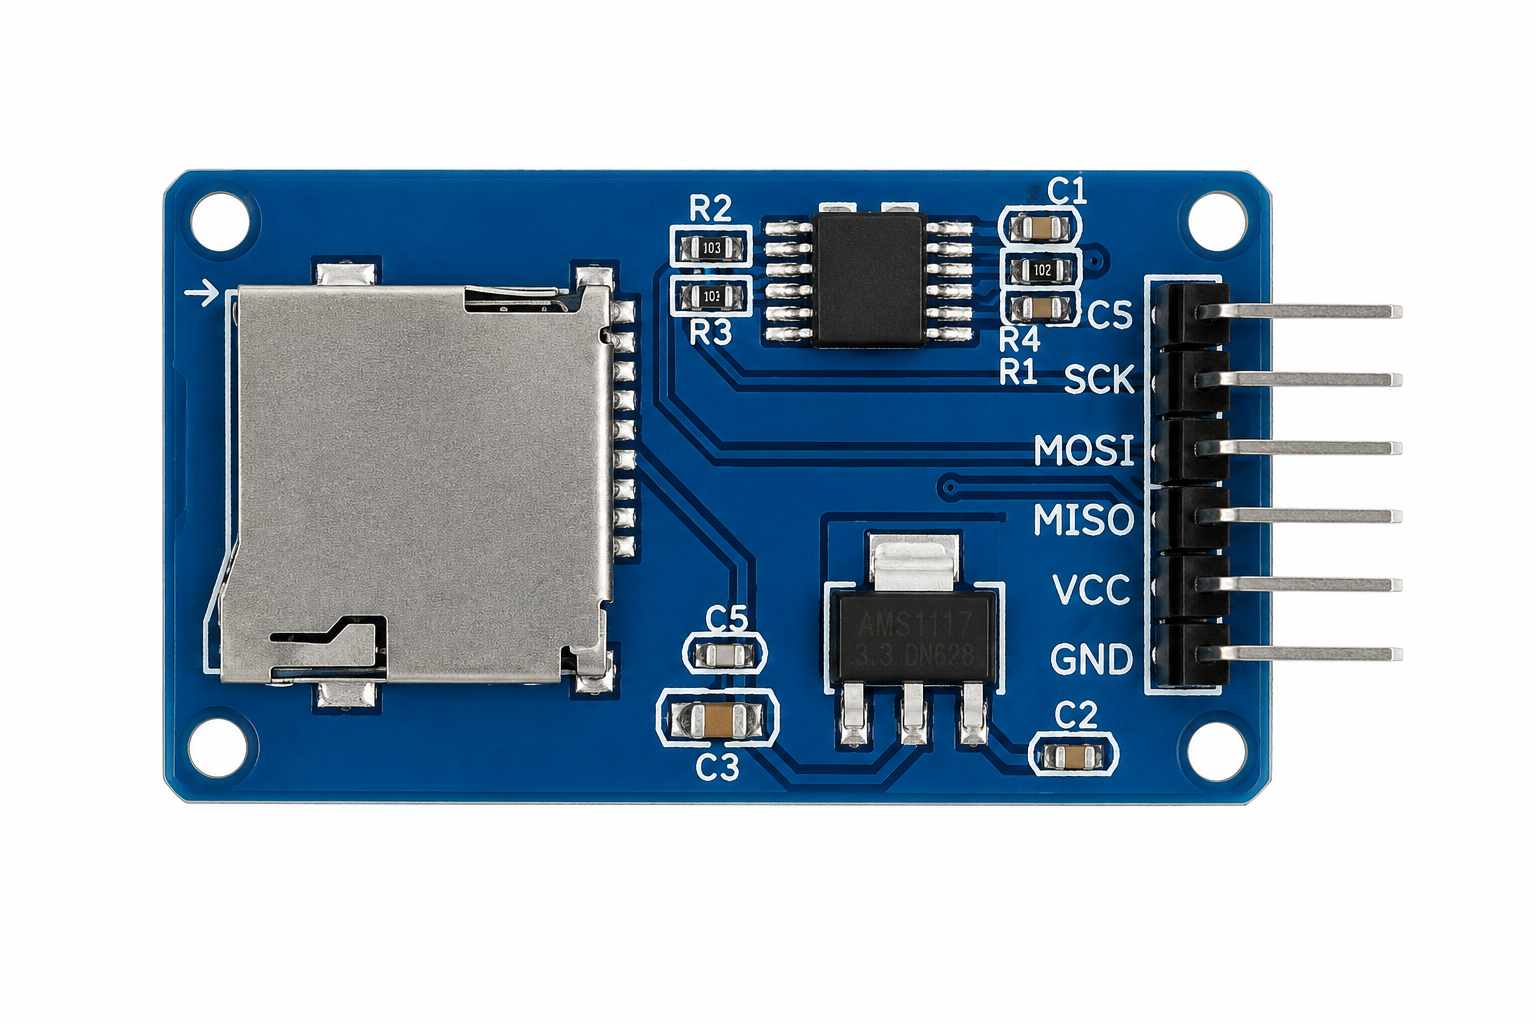
\includegraphics[width=0.30\textwidth]{figures/SdCardModule}
% TODO: copy Academic-Thesis/SystemImage/SdCardModule.png to figures/SdCardModule.png before compiling
\caption{SD card module mounted on the MAIN gateway node. The module uses the HSPI bus of the ESP32 and stores all sensor readings and system events in CSV and JSONL format, providing offline persistence between upload sessions.}
\label{fig:sd-card-module}
\end{figure}

The CSV format is used for sensor readings because it supports efficient append operations and is directly portable to analytics tools. JSONL is used for system events because each event carries a variable-length JSON object with fields that differ by event type. The SD card is the only storage mechanism; no data is held in ESP32 flash between cycles, as the deep sleep state clears RAM. Data acquisition continues uninterrupted across days or weeks without Internet access; the SD card accumulates the full measurement history until Upload Mode is manually triggered.

% ----------------------------------------------------------
\subsection{Upload Mode}
\label{sec:mode-upload}
% ----------------------------------------------------------

Upload Mode is triggered by a sustained press of the GPIO34 button on the MAIN node, requiring contact of at least one second. The sustained trigger distinguishes Upload Mode from the four-consecutive-press sequence used for RTC synchronisation and from brief accidental contact.

The mode was designed around the reality of intermittent Internet access in Saharan field environments. Continuous upload would require a persistent mobile data connection, which is neither cost-effective nor reliable at agricultural field sites. The offline-first design accumulates data locally and transfers it in a single batch when connectivity becomes temporarily available.

During Upload Mode, MAIN reads the accumulated CSV and JSONL files from the SD card and transmits their contents to the WebService backend via the POST \texttt{/api/v1/upload} endpoint. The backend processes each record by inserting sensor readings into the \texttt{sensor\_readings} table using the \texttt{measured\_at} timestamp from the SD record, and system events into the \texttt{system\_events} table using the \texttt{event\_time} field. The upload transaction's own timestamp is stored in the \texttt{uploads} table as transfer metadata. This timestamp serves as an audit record of when data was transmitted; it is not used in any analytical query, chart, or dashboard computation. The distinction is enforced in the backend ingestion logic and documented in the data-field policy described in Section~\ref{sec:storage-time}.

% ----------------------------------------------------------
\subsection{RTC Synchronisation Mode}
\label{sec:mode-rtc-sync}
% ----------------------------------------------------------

RTC Synchronisation Mode corrects the DS3231 real-time clock when the stored time has drifted or when the battery was replaced. Measurement timestamps are derived exclusively from the DS3231; any persistent drift would introduce systematic errors in the \texttt{measured\_at} values for all readings acquired before the correction.

\begin{figure}[H]
\centering
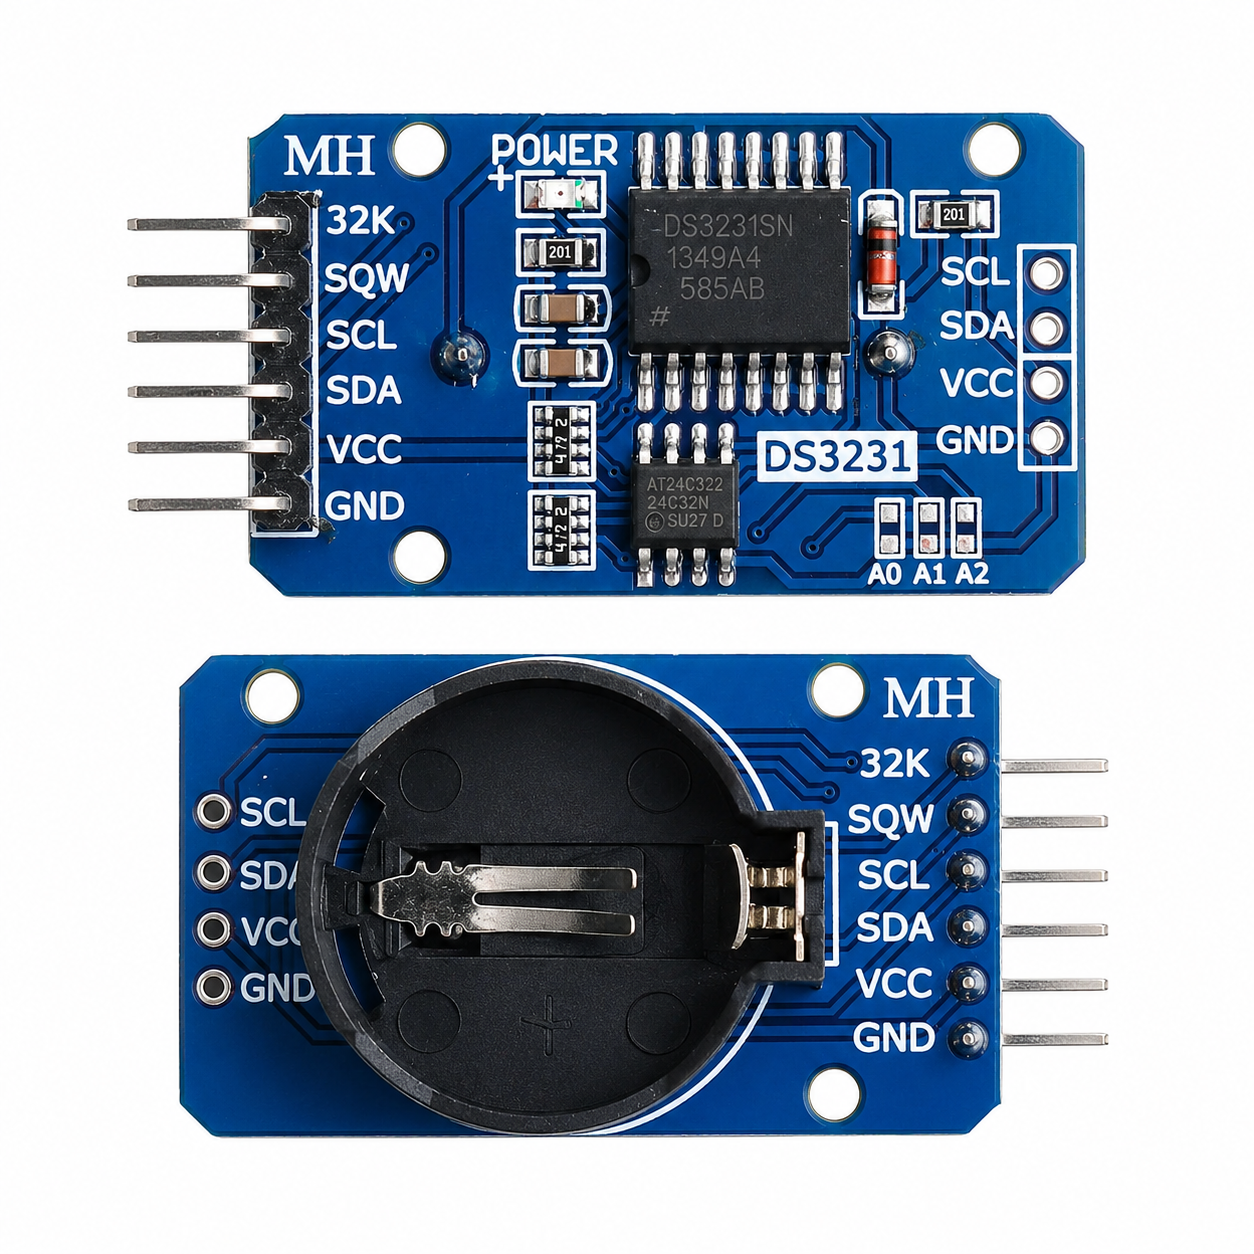
\includegraphics[width=0.30\textwidth]{figures/Rtc}
% TODO: copy Academic-Thesis/SystemImage/Rtc.png to figures/Rtc.png before compiling
\caption{DS3231 RTC module mounted on the MAIN gateway node. The module provides battery-backed timekeeping and is the exclusive source of \texttt{measured\_at} timestamps for all sensor readings.}
\label{fig:rtc-module}
\end{figure}

The mode is triggered by four consecutive short presses of the GPIO34 button. MAIN initiates a connection to the WebService backend and sends a synchronisation request. The backend responds with the current server time in the \texttt{server\_time} field of the JSON response. MAIN parses this value and writes it to the DS3231 over I2C. All subsequent readings are timestamped from the updated clock. The synchronisation event is logged to the SD card and transmitted to the backend as a system event, providing an audit record of when the RTC was last corrected.

% ----------------------------------------------------------
\subsection{Diagnostic Logging Mode}
\label{sec:mode-diagnostic}
% ----------------------------------------------------------

Diagnostic Logging Mode is not a separate operating state but a cross-cutting concern active throughout all other modes. Whenever a noteworthy event occurs — a failed ACK, a node entering recovery, a successful recovery, a node marked as no longer communicating, an SD write error, a sensor read failure, or an upload transaction — the MAIN node writes a structured record to the JSONL event file on the SD card.

These event records carry a type field (for example: \texttt{recovery\_started}, \texttt{recovery\_cycle\_adjusted}, \texttt{recovery\_success}, \texttt{recovery\_failed}, \texttt{node\_marked\_dead}, \texttt{node\_back\_online}), a \texttt{event\_time} derived from the DS3231, and a payload containing mode-specific context. During upload, the event records are transmitted to the backend alongside sensor readings and stored in the \texttt{system\_events} table. The dashboard's diagnostics view draws from this table to present a timeline of system health events to the operator.

The logging mechanism serves a dual purpose. During field testing, it enabled the diagnosis of the timing-drift failure that motivated Recovery Mode. In production use, it provides the operator with evidence to distinguish sensor malfunction, communication outage, and firmware-level issues without physical access to the node.

\bigskip

Table~\ref{tab:firmware-operating-modes} consolidates the eight firmware modes with their trigger conditions, field motivations, and outputs.

\begin{table}[H]
\centering
\caption{Firmware operating modes of the proposed system, showing trigger conditions, motivations, and outputs.}
\label{tab:firmware-operating-modes}
\small
\begin{tabular}{p{2.5cm} p{2.8cm} p{3.0cm} p{3.2cm} p{2.5cm}}
\hline
\textbf{Mode} & \textbf{Trigger} & \textbf{Purpose} & \textbf{Field problem addressed} & \textbf{Output / log} \\
\hline
Normal Sensing & Superframe timer wake & Scheduled sensor acquisition and SD storage & Periodic monitoring without continuous power & CSV reading row; SD write \\
\hline
Power Saving & Always active between cycles & Deep sleep, relay power control, BME280 forced mode & Battery longevity in off-grid deployment & Reduced active duty cycle \\
\hline
LoRa RX/ACK & MAIN receive window open & Receive remote node packets; send ACK with RTC time & Loss of remote data without confirmation feedback & SD write; ACK packet; \texttt{node\_back\_online} event \\
\hline
Recovery & ACK failure increments \texttt{txFailCount} & Adaptive sleep adjustment to re-enter MAIN window & Timing drift causing persistent missed cycles & JSONL event: \texttt{recovery\_started}, \texttt{recovery\_cycle\_adjusted}, \texttt{recovery\_success}, \texttt{recovery\_failed} \\
\hline
Local Storage & End of each sensing cycle & Persist readings and events to SD & Data loss during Internet-unavailable periods & CSV row appended; JSONL event appended \\
\hline
Upload & Long button press ($\geq$1~s) & Batch transfer of SD content to backend & Continuous upload impractical at field site & POST to \texttt{/api/v1/upload}; \texttt{uploads} table row; upload JSONL event \\
\hline
RTC Synchronisation & Four consecutive button presses & Correct DS3231 clock drift; server time written & Drift in measurement timestamps over weeks & RTC updated; sync event logged \\
\hline
Diagnostic Logging & Continuous (all modes) & Record system health events with timestamps & No remote visibility into node/gateway health & JSONL event file; \texttt{system\_events} table row \\
\hline
\end{tabular}
\end{table}

% ============================================================
\section{Communication Design}
\label{sec:ch3-communication}
% ============================================================

All wireless communication in the system uses LoRa, a spread-spectrum modulation technique operating at 433~MHz in the ISM band. The physical layer parameters are configured identically on all three nodes to ensure mutual decoding: spreading factor SF7, bandwidth 125~kHz, coding rate 4/5, CRC enabled, and transmit power 14~dBm. SF7 was chosen to balance airtime, energy per packet, and link budget for the distances anticipated between nodes and the MAIN gateway in the target agricultural field. The justification for the LoRa selection was established in Section~\ref{sec:communication}.

\begin{figure}[H]
\centering
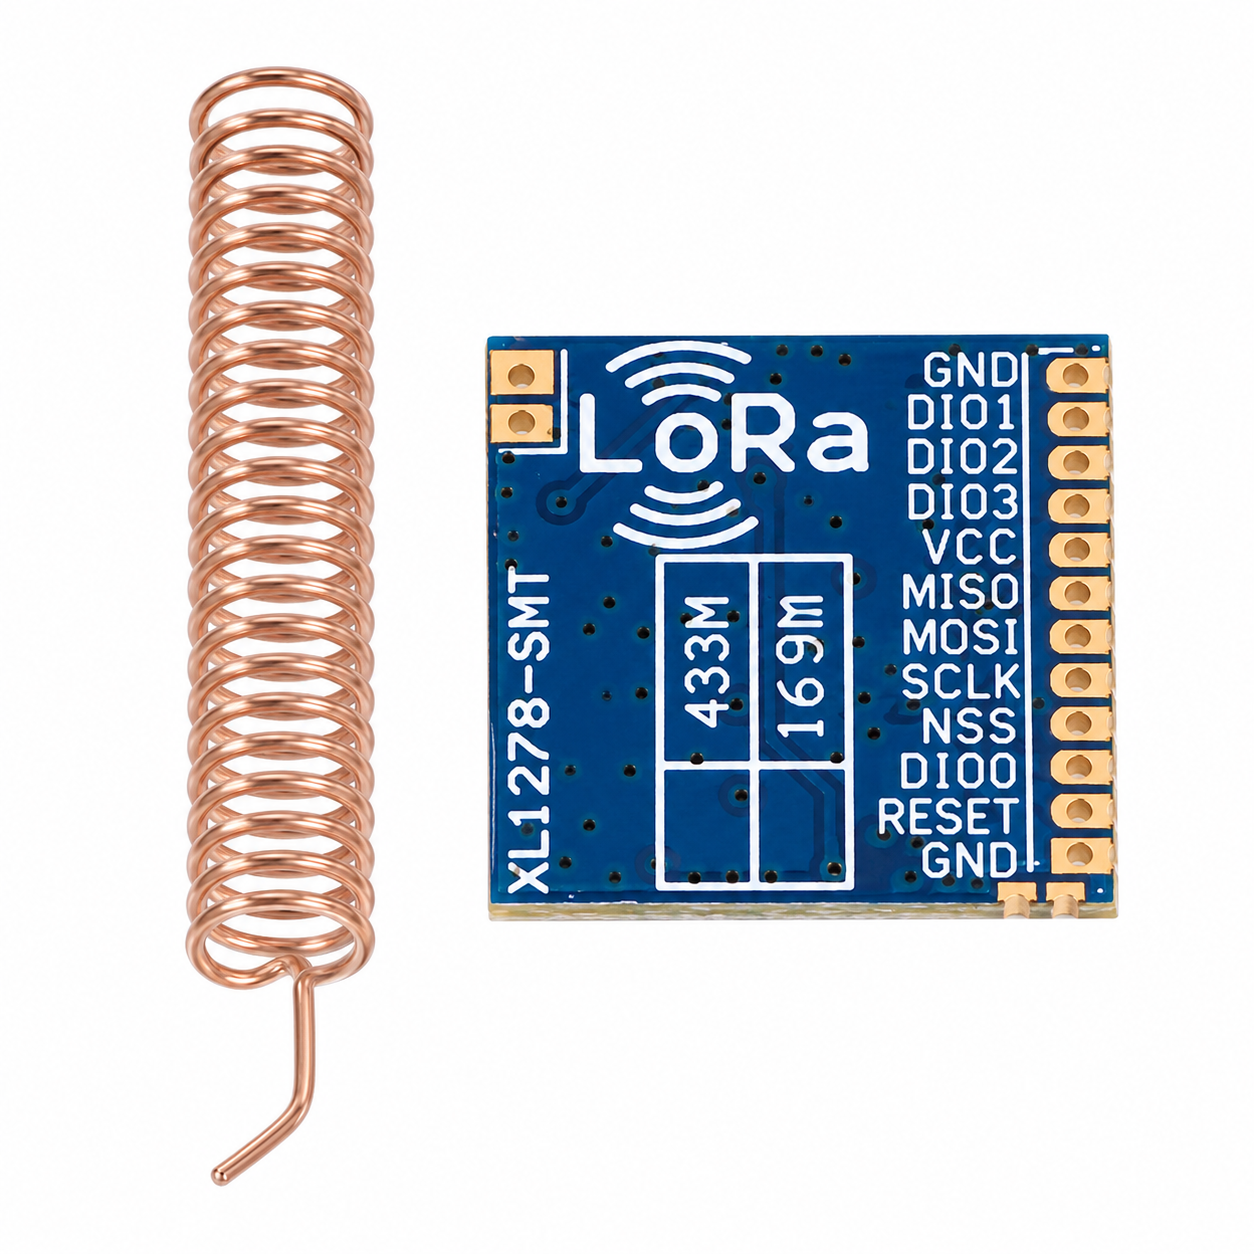
\includegraphics[width=0.35\textwidth]{figures/LoRa}
% TODO: copy Academic-Thesis/SystemImage/LoRa.png to figures/LoRa.png before compiling
\caption{SX127x LoRa transceiver module used on all three nodes. The module operates at 433~MHz and is configured with identical parameters across the system to ensure compatibility between the transmitting remote nodes and the receiving MAIN gateway.}
\label{fig:lora-module-ch3}
\end{figure}

Communication follows a structured superframe pattern rather than contention-based access. Node2 transmits first, at approximately 24~seconds into the ten-minute frame. Node3 transmits at approximately 38~seconds. MAIN's receive window spans the first 70~seconds of the frame, providing margin for each node. Because only one node transmits during each sub-window, collision risk is minimal under normal operation.

\begin{figure}[H]
\centering
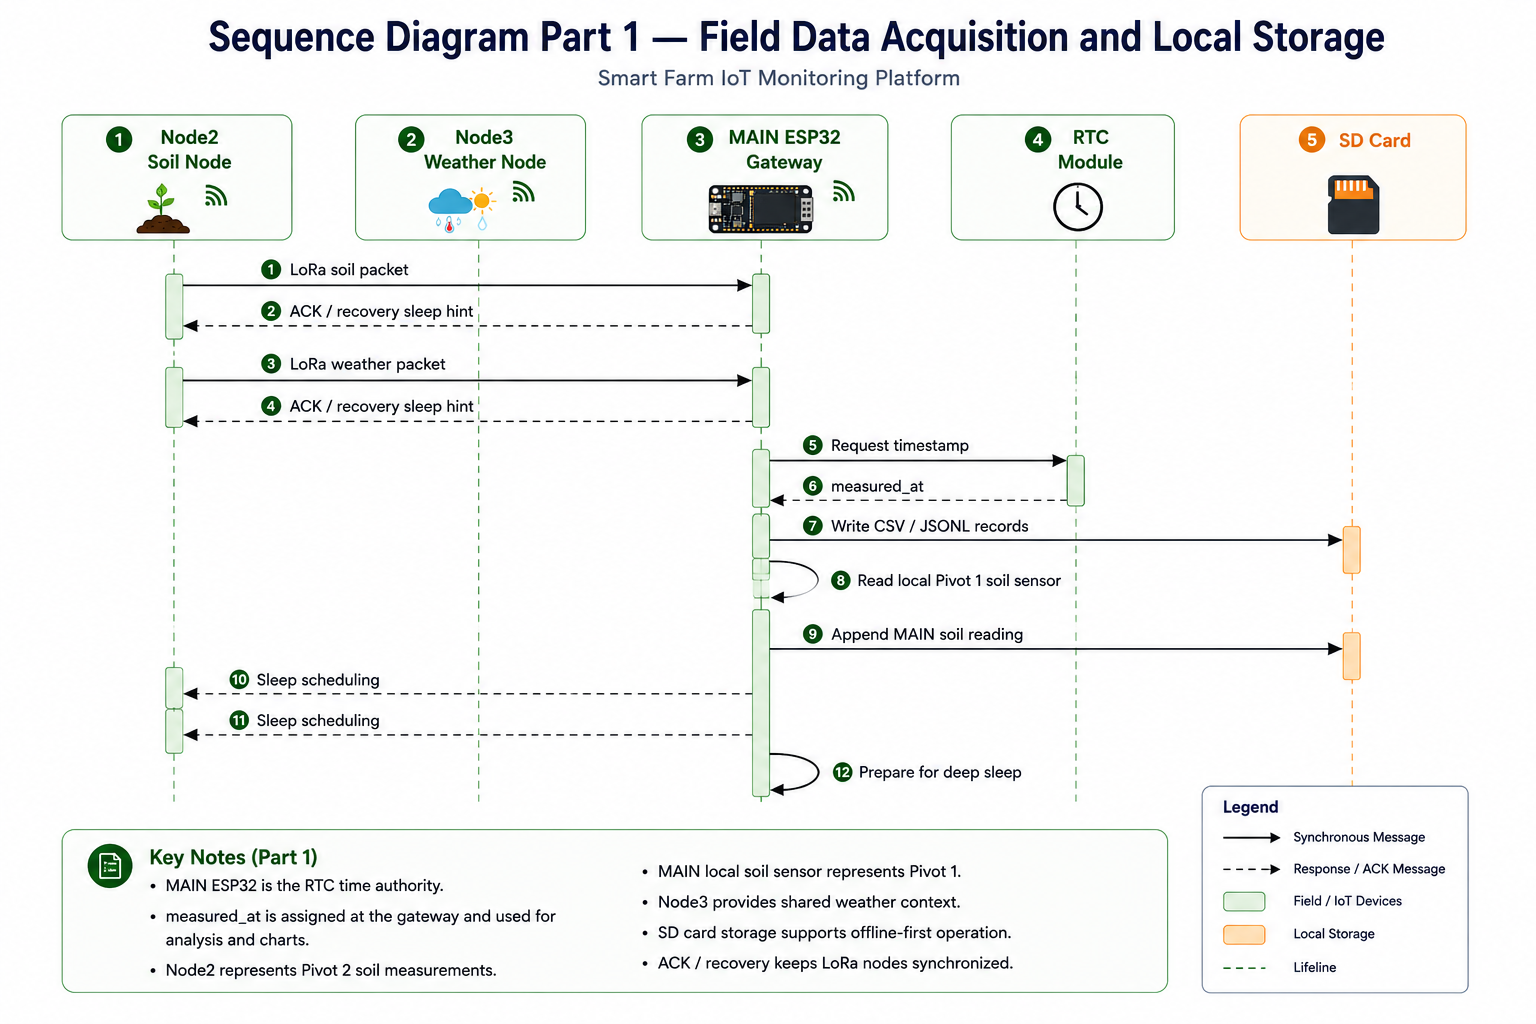
\includegraphics[width=\textwidth]{figures/SequenceDiagram1}
% TODO: confirm whether Academic-Thesis/Diagrams/Sequence Diagrams.png is one file or two separate files (Sequence Diagrams 1.png and Sequence Diagrams 2.png); copy the appropriate file(s) to figures/SequenceDiagram1.png before compiling
\caption{Sequence diagram illustrating the LoRa communication flow during a normal sensing cycle, showing Node2 and Node3 transmissions, MAIN reception and acknowledgement, local soil read, and SD storage sequence.}
\label{fig:sequence-diagram-1}
\end{figure}

\begin{figure}[H]
\centering
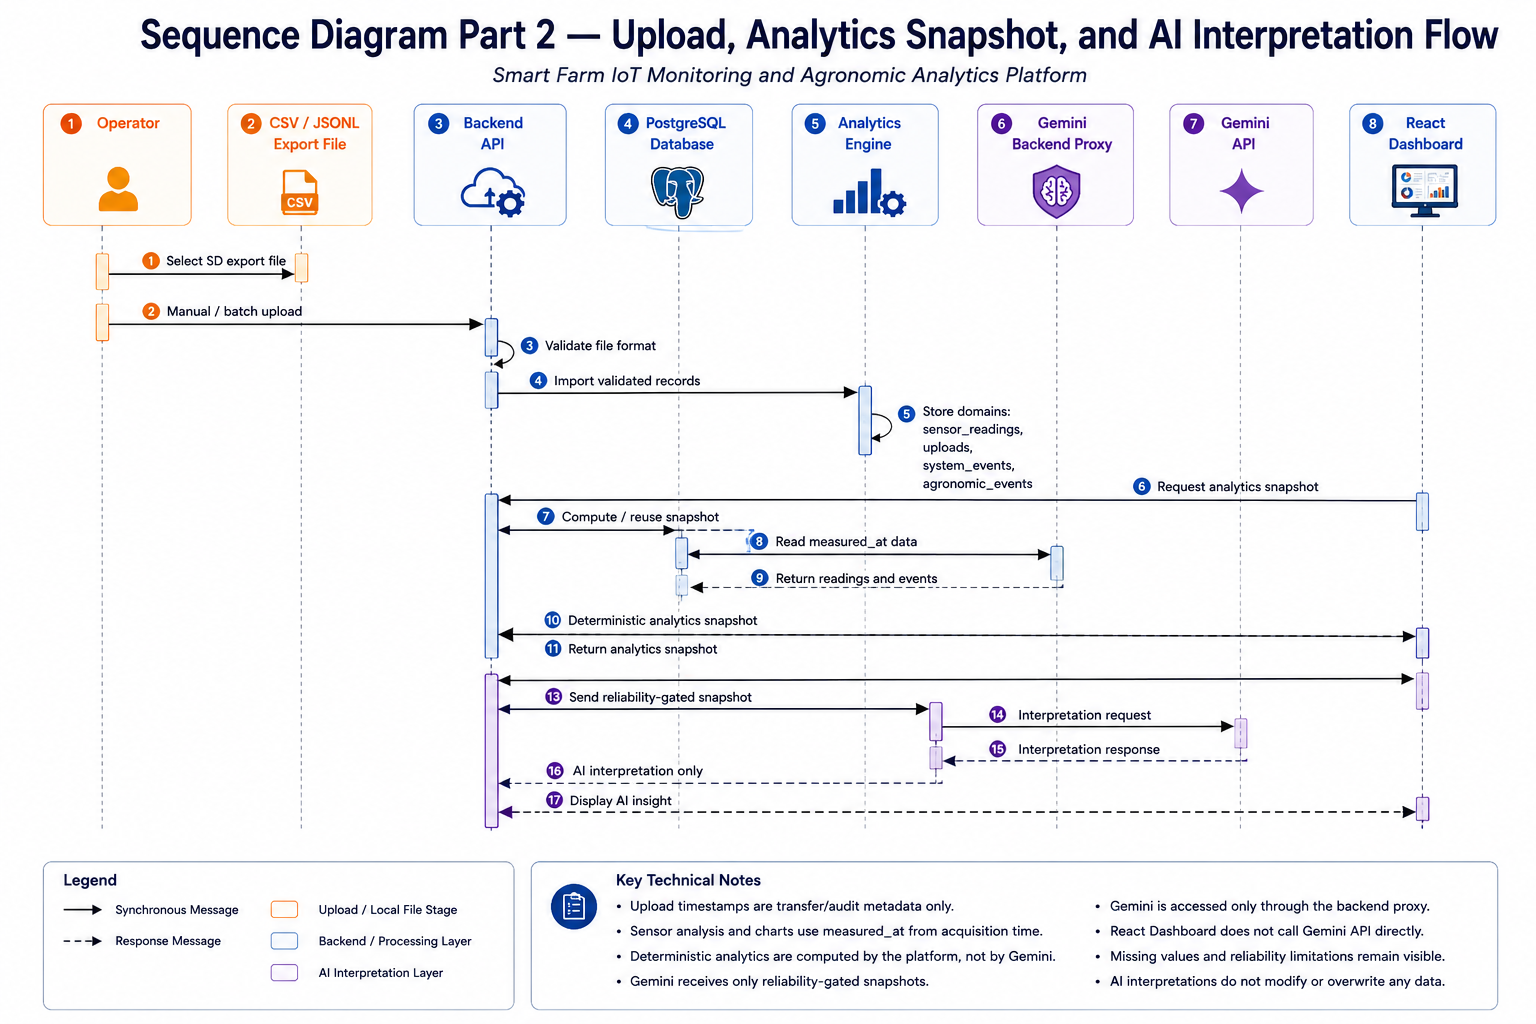
\includegraphics[width=\textwidth]{figures/SequenceDiagram2}
% TODO: confirm whether a second sequence diagram file exists for the recovery and upload flows; copy to figures/SequenceDiagram2.png if confirmed; otherwise remove this figure and its reference
\caption{Sequence diagram illustrating the communication sequence during Recovery Mode, showing the adaptive retry mechanism when a remote node fails to receive an ACK, and the eventual re-synchronisation with the MAIN receive window.}
\label{fig:sequence-diagram-2}
\end{figure}

Each LoRa packet carries a structured payload. The payload includes a node identifier, the sensor measurement values (three integers from the Modbus register map for soil nodes; three floats from the BME280 for the weather node), a firmware stage constant indicating the node's progress through the superframe, and a CRC byte for payload integrity. MAIN decodes the node identifier, validates the CRC, and stamps the packet with \texttt{measured\_at} from the DS3231 before writing the reading to SD.

The ACK packet is transmitted by MAIN within the receive window immediately after a successful packet decode. It carries the current RTC timestamp and an echo of the source node identifier. If a node does not receive the ACK within 1500~milliseconds of its own transmission, it registers a miss and the Recovery Mode logic described in Section~\ref{sec:mode-recovery} applies on the next cycle.

The RSSI values recorded in the validation dataset (spanning the range from approximately $-76$~dBm to $-97$~dBm across the observation window) confirm that functional communication was maintained between the nodes and the MAIN gateway throughout the validation period. Formal range characterisation over measured distances was not conducted; the system is not described in terms of a guaranteed communication range.

% ============================================================
\section{Data Storage and Time Policy}
\label{sec:storage-time}
% ============================================================

The data model of the system is organised into four canonical domains, each with a distinct time field that reflects the semantic role of the domain. The policy governing these fields is enforced at every layer of the implementation, from firmware SD writes through backend ingestion to dashboard queries.

The central principle of the time policy is that the time of measurement and the time of upload are distinct and must never be conflated. This distinction was identified in Chapter~\ref{chap:related-works} as a gap in several reviewed systems, where upload timestamps were used as proxies for measurement time in stored records and dashboard charts. In the proposed system, the \texttt{measured\_at} field is written by the MAIN gateway firmware from the DS3231 RTC at the moment a packet is received and validated; it is not modifiable by subsequent processing steps. The \texttt{uploaded\_at} field in the \texttt{uploads} table records when the SD batch was transmitted to the backend; it is stored as transfer audit metadata and is not referenced in any analytical query, chart computation, or dashboard visualisation.

\begin{table}[H]
\centering
\caption{Data domains, primary time fields, and analytical roles in the proposed storage model.}
\label{tab:data-domains-time-fields}
\small
\begin{tabular}{p{3.0cm} p{4.0cm} p{2.8cm} p{1.5cm} p{3.0cm}}
\hline
\textbf{Data domain} & \textbf{Stored content} & \textbf{Primary time field} & \textbf{Used for analytics?} & \textbf{Purpose} \\
\hline
\texttt{sensor\_readings} & Soil moisture, soil temperature, soil EC, air temperature, air humidity, barometric pressure & \texttt{measured\_at} (DS3231 RTC) & Yes & Trend charts, quality checking, reliability scoring, threshold alerts \\
\hline
\texttt{system\_events} & Recovery events, upload events, node status changes, sensor errors, SD errors & \texttt{event\_time} (DS3231 RTC) & Yes (diagnostics only) & System health timeline; diagnostics dashboard panel \\
\hline
\texttt{uploads} & Upload transaction metadata; SD batch reference; record counts & \texttt{uploaded\_at} (server time of receipt) & No — transfer audit metadata only & Audit trail of when SD batches were transmitted; never used as measurement time \\
\hline
\texttt{agronomic\_events} & Irrigation sessions, harvest events, fertilisation records, operator notes & \texttt{started\_at} / \texttt{ended\_at} (operator-entered) & Yes (agronomic context layer) & Contextual overlay on measurement charts; agronomic timeline \\
\hline
\end{tabular}
\end{table}

The upload timestamp is transfer and audit metadata only. It is recorded to provide a traceable log of when each SD batch was received by the backend, supporting diagnosis of upload failures and data completeness checks. It does not appear on any measurement chart axis, is not used in any filtering or aggregation query on sensor readings, and is never presented to the operator as an approximation of when a measurement was taken. This separation is not merely a policy declaration; it is enforced structurally in the backend ingestion logic: the upload endpoint inserts each reading using the \texttt{measured\_at} value from the SD record, and the upload transaction's own timestamp is stored exclusively in the \texttt{uploads} table, which is not joined to the \texttt{sensor\_readings} table in any analytical query.

All timestamps are stored in UTC at the database level. The dashboard converts UTC values to Algeria Standard Time (UTC+1) for display, as documented in the backend configuration. Agronomic event times are entered by the operator through the dashboard interface; they are stored in the \texttt{agronomic\_events} table with separate \texttt{started\_at} and \texttt{ended\_at} fields to support duration-based queries and chart overlay rendering.

% ============================================================
\section{Backend Implementation}
\label{sec:backend}
% ============================================================

The backend is implemented as a Node.js application using the Express.js framework, connected to a PostgreSQL relational database. It exposes a REST API secured by an API key, consumed by both the MAIN gateway firmware during Upload Mode and the React web dashboard for data retrieval and display.

The backend serves three categories of client requests. The firmware upload client issues POST requests to transmit SD batch content after each Upload Mode session. The dashboard client issues GET requests to retrieve readings, events, analytics snapshots, and agronomic events for display. Administrative clients may issue POST requests to create or update agronomic events through the dashboard interface.

\begin{figure}[H]
\centering
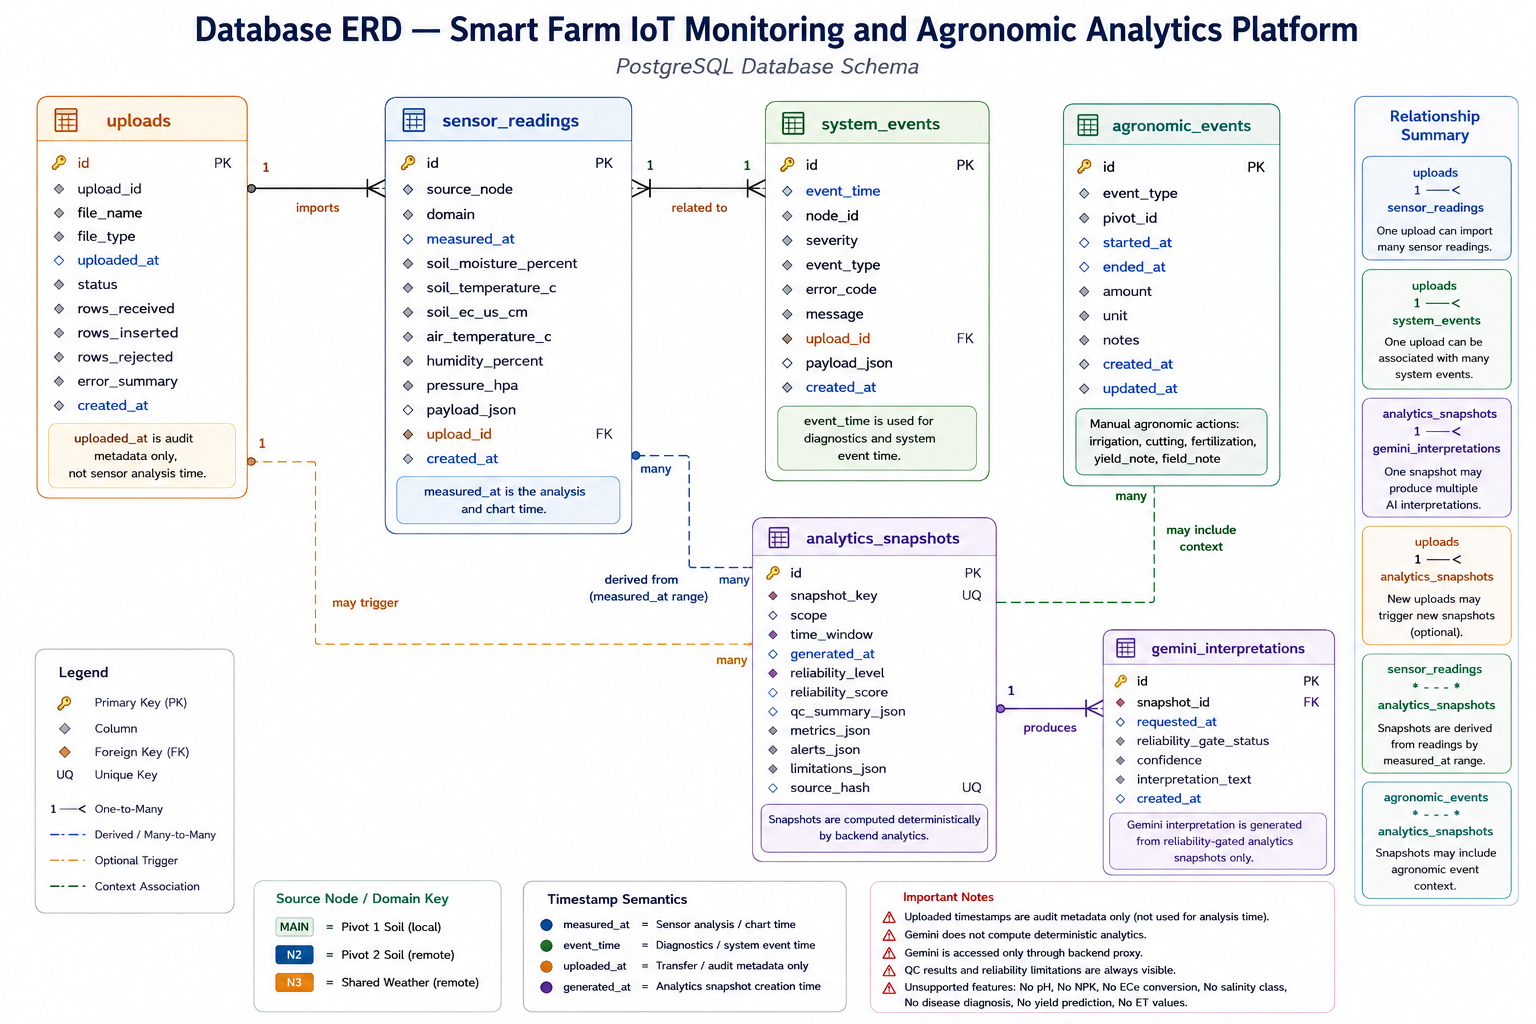
\includegraphics[width=\textwidth]{figures/DatabaseERDDiagram}
% TODO: copy Academic-Thesis/Diagrams/DatabaseERDDiagram.png to figures/DatabaseERDDiagram.png before compiling
\caption{Entity-relationship diagram of the PostgreSQL database, showing the \texttt{gateways}, \texttt{nodes}, \texttt{sensor\_readings}, \texttt{system\_events}, \texttt{uploads}, \texttt{agronomic\_events}, and \texttt{analytics\_snapshots} tables and their relationships.}
\label{fig:database-erd}
\end{figure}

The database schema is organised in four SQL migration files. The initial migration (\texttt{001\_init.sql}) creates the \texttt{gateways}, \texttt{nodes}, \texttt{sensor\_readings}, \texttt{system\_events}, and \texttt{uploads} tables. A patch migration (\texttt{002\_patch.sql}) applies corrections to column definitions. The agronomic migration (\texttt{003\_agronomic.sql}) adds the \texttt{agronomic\_events} table. The analytics migration (\texttt{004\_analytics\_snapshots.sql}) adds the \texttt{analytics\_snapshots} table, which stores the output of the deterministic analytics pipeline described in Part~B. Table~\ref{tab:database-tables} summarises the implemented tables and their roles.

\begin{table}[H]
\centering
\caption{PostgreSQL database tables implemented in the WebService backend.}
\label{tab:database-tables}
\small
\begin{tabular}{p{3.8cm} p{2.5cm} p{7.0cm}}
\hline
\textbf{Table} & \textbf{Migration} & \textbf{Purpose and key fields} \\
\hline
\texttt{gateways} & 001\_init & Registered MAIN gateway devices; gateway identifier, name, API key hash \\
\hline
\texttt{nodes} & 001\_init & Registered remote nodes; node identifier, gateway reference, node type \\
\hline
\texttt{sensor\_readings} & 001\_init & All sensor measurements; \texttt{measured\_at} (RTC-derived), soil and weather values, node reference \\
\hline
\texttt{system\_events} & 001\_init & Firmware diagnostic events; \texttt{event\_time} (RTC-derived), event type, payload \\
\hline
\texttt{uploads} & 001\_init & Upload transaction records; \texttt{uploaded\_at} (server receipt time), record counts, gateway reference; transfer audit metadata only \\
\hline
\texttt{agronomic\_events} & 003\_agronomic & Operator-recorded field events; \texttt{started\_at}, \texttt{ended\_at}, event type, notes \\
\hline
\texttt{analytics\_snapshots} & 004\_analytics & Output of deterministic analytics pipeline; snapshot timestamp, quality scores, reliability indicator, alert flags \\
\hline
\end{tabular}
\end{table}

The upload ingestion process follows a defined sequence. The firmware transmits a JSON body containing arrays of sensor reading objects and system event objects, each carrying the time fields written by the firmware to SD. The backend validates the API key, creates an \texttt{uploads} record with the server receipt timestamp, then iterates over each reading object and inserts a row into \texttt{sensor\_readings} using the \texttt{measured\_at} value from the firmware-provided object. System events are inserted into \texttt{system\_events} using the \texttt{event\_time} value from the firmware-provided object. At no point does the backend substitute the upload receipt timestamp for any measurement-derived time field.

\begin{table}[H]
\centering
\caption{Backend REST API endpoints and their functions.}
\label{tab:api-endpoints}
\small
\begin{tabular}{p{1.5cm} p{4.5cm} p{2.5cm} p{5.0cm}}
\hline
\textbf{Method} & \textbf{Endpoint} & \textbf{Client} & \textbf{Function} \\
\hline
POST & \texttt{/api/v1/upload} & Firmware (Upload Mode) & Ingest SD batch; insert readings, events, uploads; return server time for optional RTC sync \\
\hline
GET & \texttt{/api/v1/readings} & Dashboard & Retrieve sensor readings filtered by node, time range, and measurement domain \\
\hline
GET & \texttt{/api/v1/events} & Dashboard & Retrieve system events for diagnostics timeline \\
\hline
GET & \texttt{/api/v1/agronomic-events} & Dashboard & Retrieve agronomic events for chart overlay and event log \\
\hline
POST & \texttt{/api/v1/agronomic-events} & Dashboard & Create a new agronomic event record \\
\hline
GET & \texttt{/api/v1/analytics} & Dashboard & Retrieve analytics snapshots for the Processed Data Viewer \\
\hline
POST & \texttt{/api/v1/gemini} & Dashboard & Forward deterministic snapshot to Gemini and return narrative response; AI boundary enforced \\
\hline
\end{tabular}
\end{table}

% TODO: add captured API response samples if available — see missing_items H5

The \texttt{/api/v1/gemini} endpoint enforces the AI interpretation boundary described in the system requirements. The endpoint receives the deterministic analytics snapshot computed by the backend pipeline, not raw sensor readings, and forwards it to the Gemini model via the Google AI API. The model is not given access to the raw database, is not asked to compute statistics, and is not instructed to produce agronomic prescriptions. The response is returned to the dashboard and presented to the operator under a label that identifies it as an AI-generated interpretive narrative. The analytical layer — quality scores, reliability indicator, and threshold alerts — is computed entirely by the deterministic pipeline and is not modified by the AI response.

% ============================================================
\section{Dashboard Implementation}
\label{sec:dashboard}
% ============================================================

The web dashboard is implemented as a React application built with the Vite toolchain and TypeScript. It serves as the visualization and monitoring layer of the system, presenting uploaded and processed data to the operator through a set of purpose-built interface pages. The dashboard does not establish a persistent sensor connection or stream data in real time; it reflects the state of the backend database at the point of the most recent upload session. This design follows from the offline-first architecture described in Section~\ref{sec:storage-time}: connectivity is intermittent, and the authoritative measurement record resides on the SD card until an upload session transfers it to the backend.

\begin{figure}[H]
\centering
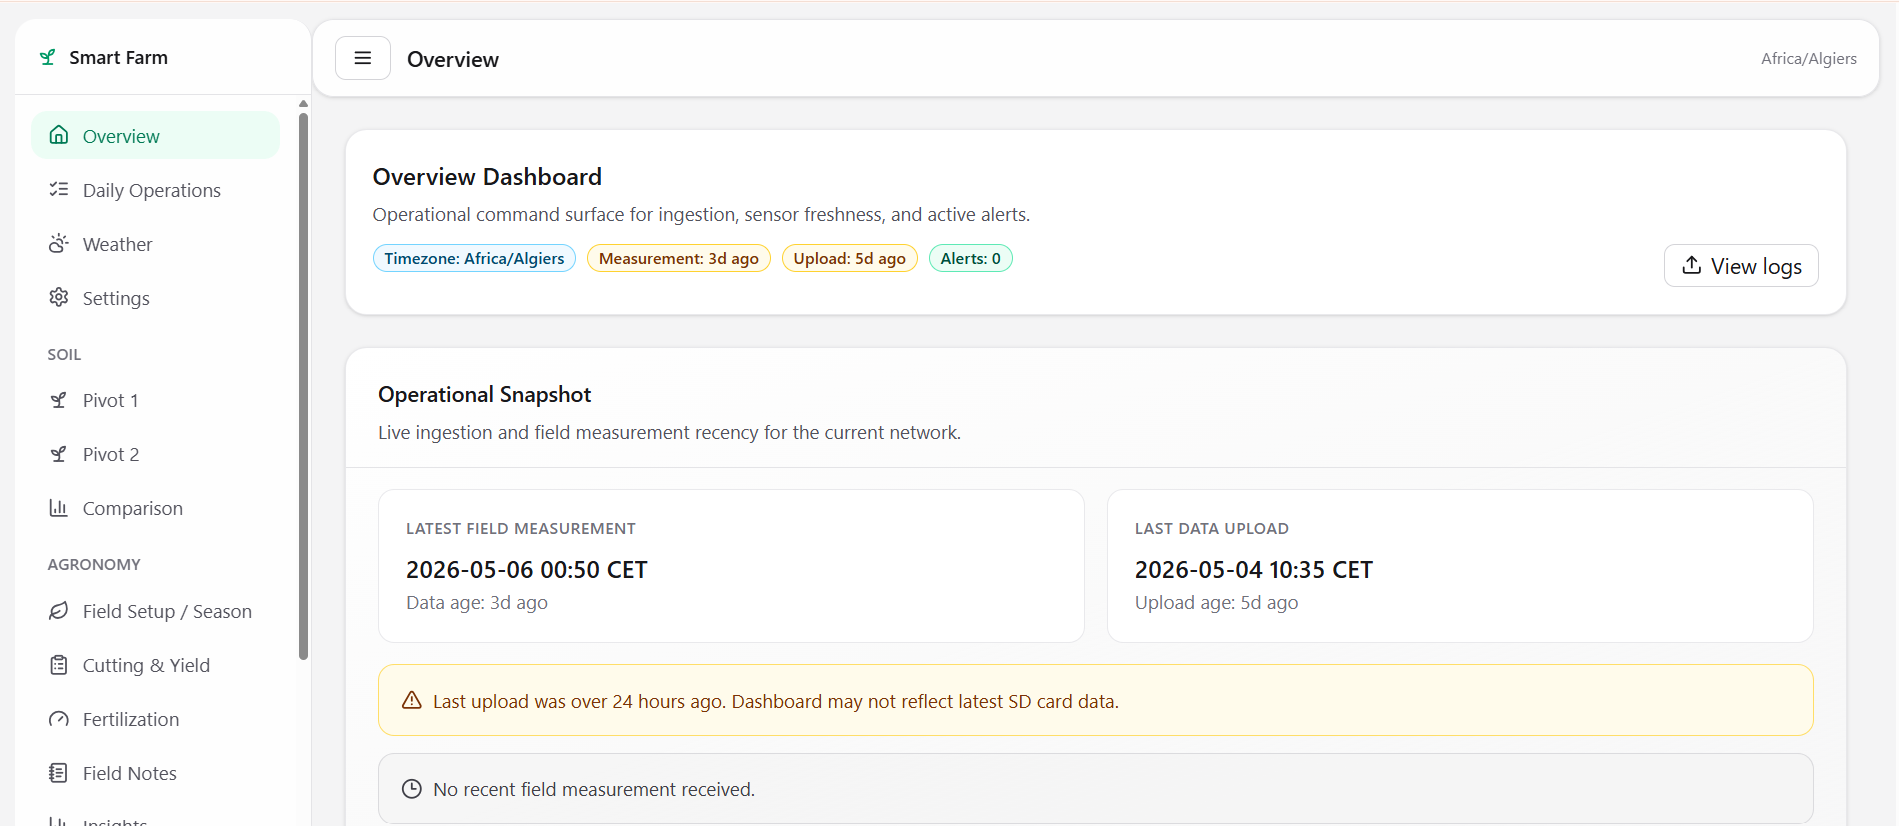
\includegraphics[width=\textwidth]{figures/DashOverview}
% TODO: copy Academic-Thesis/DashBoredImages/Overview.png to figures/DashOverview.png before compiling
\caption{Dashboard overview page presenting a summary of the latest uploaded sensor readings, system status, and navigation to domain-specific pages.}
\label{fig:dashboard-overview}
\end{figure}

The overview page provides a consolidated summary of the latest sensor values received from the three nodes, alongside navigation to domain-specific pages. It does not display a live sensor feed; instead, it reflects the most recently ingested batch, allowing the operator to confirm that the last upload session was successful before proceeding to detailed analysis.

\begin{figure}[H]
\centering
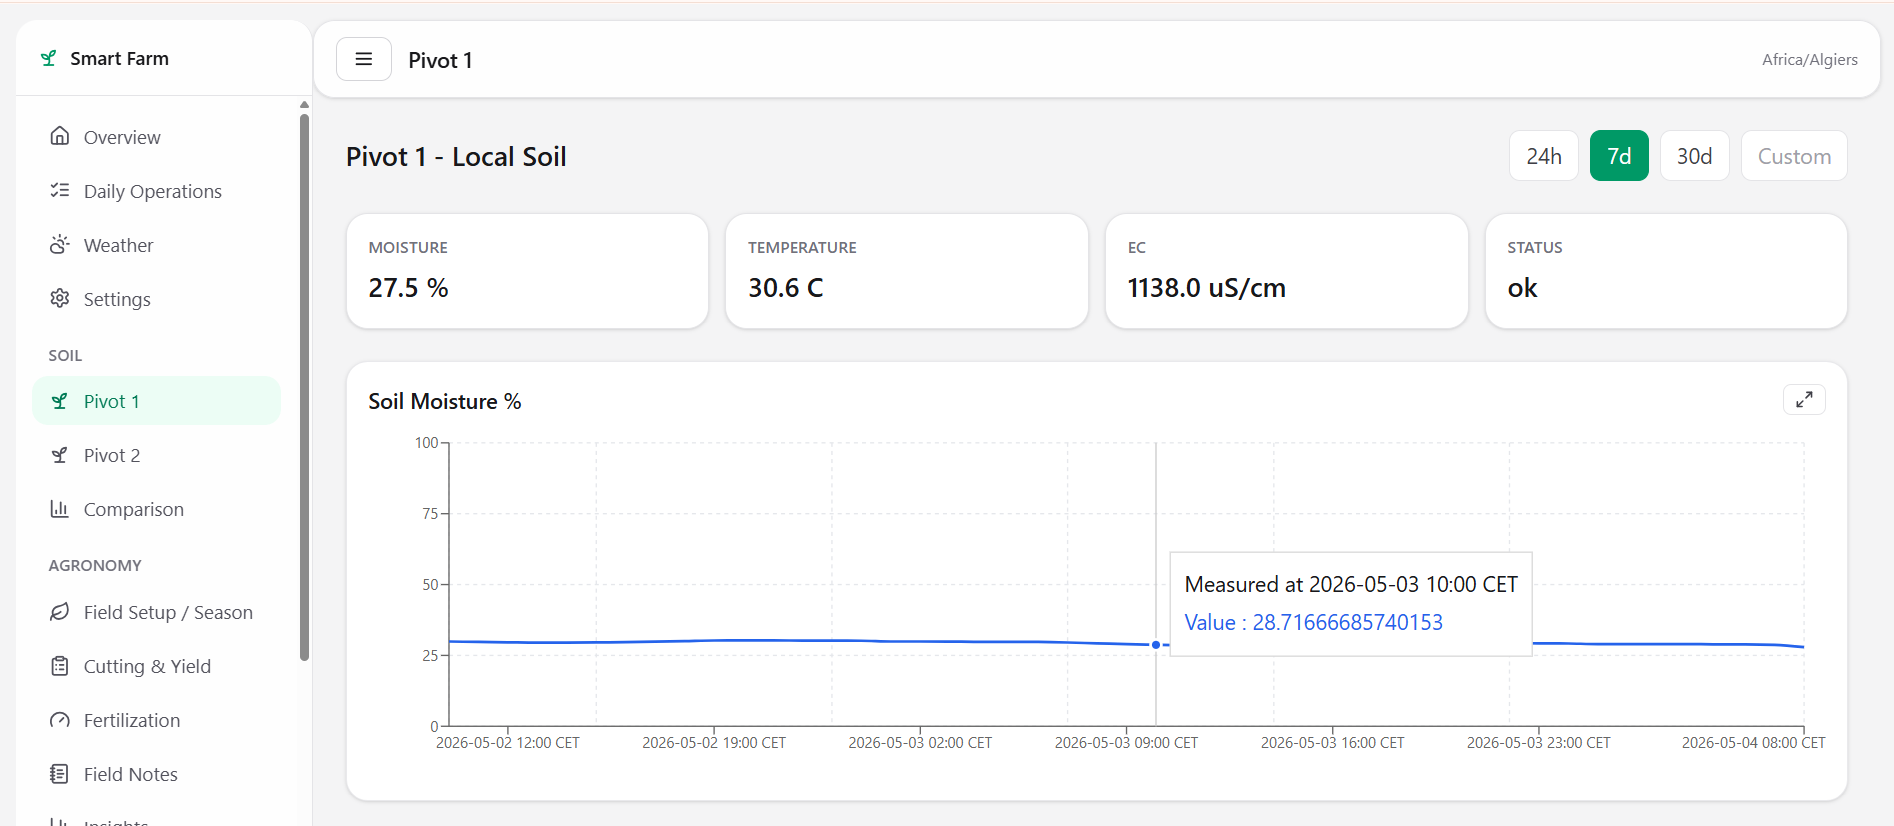
\includegraphics[width=\textwidth]{figures/DashPivot}
% TODO: copy Academic-Thesis/DashBoredImages/Pivot.png to figures/DashPivot.png before compiling
\caption{Pivot soil monitoring page displaying soil moisture, temperature, and electrical conductivity trends from Node2 (Pivot~2 remote soil sensor), with time axis derived from \texttt{measured\_at} timestamps.}
\label{fig:pivot-soil-dashboard}
\end{figure}

The pivot soil monitoring page presents time-series charts for the soil measurement dimensions: moisture, temperature, and EC. Chart time axes are populated from the \texttt{measured\_at} field in the \texttt{sensor\_readings} table, consistent with the time policy established in Section~\ref{sec:storage-time}. The upload timestamp is not used as a chart axis value at any point in the rendering pipeline.

\begin{figure}[H]
\centering
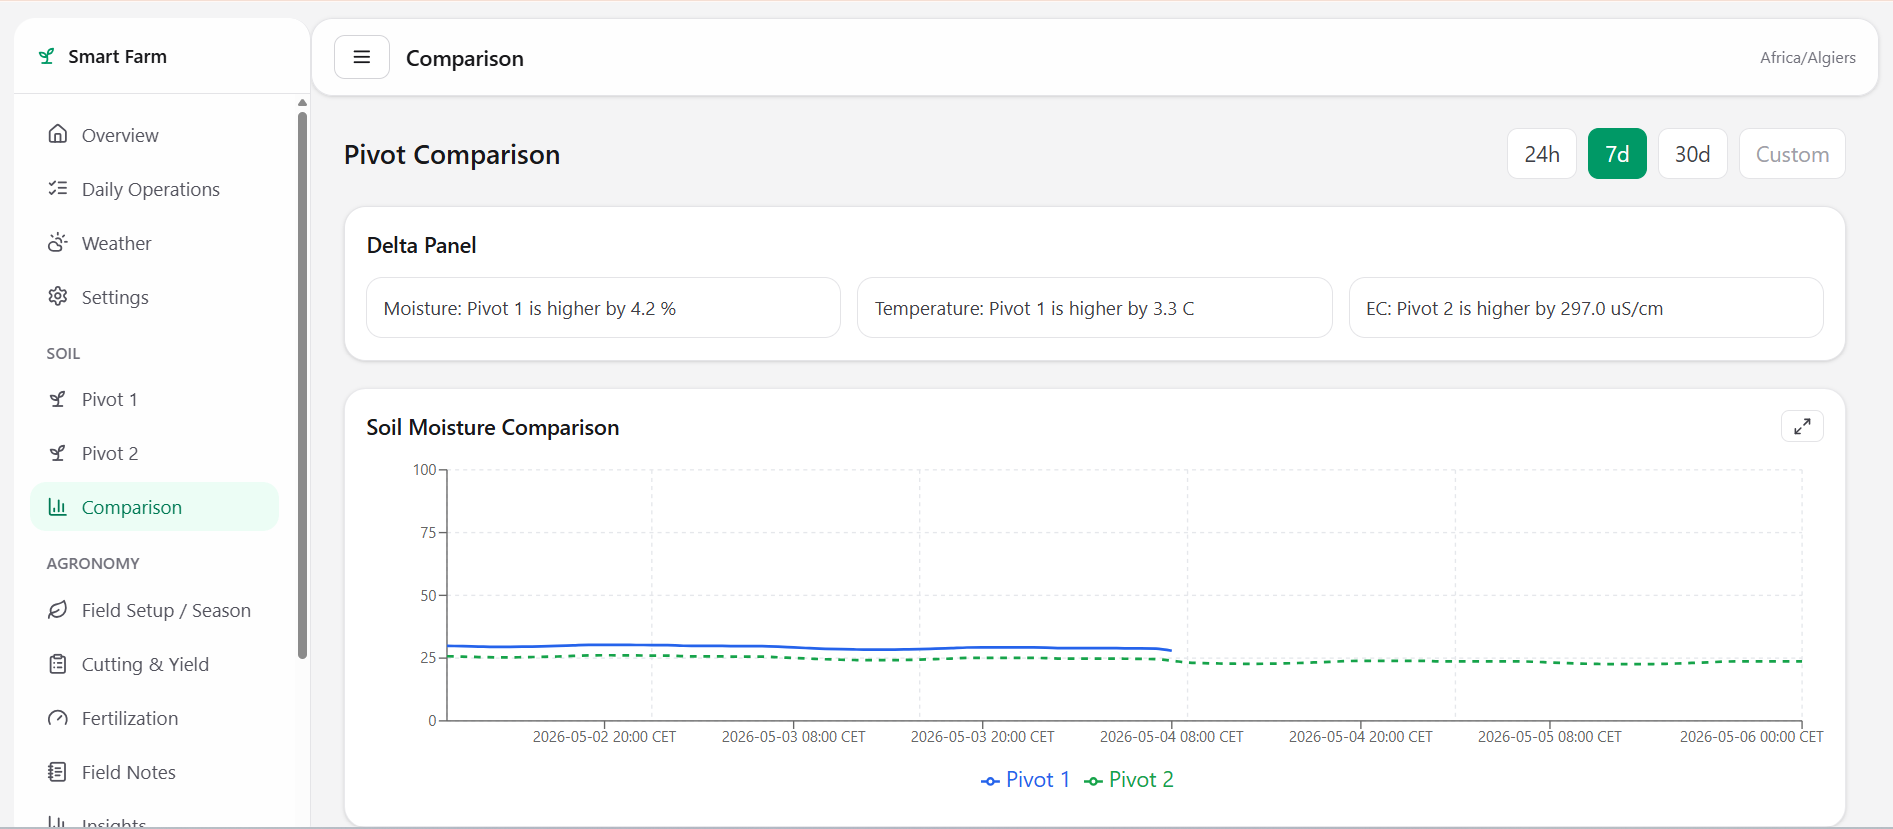
\includegraphics[width=\textwidth]{figures/DashComparison}
% TODO: copy Academic-Thesis/DashBoredImages/Comparison.png to figures/DashComparison.png before compiling
\caption{Pivot comparison page presenting side-by-side soil metric trends for Pivot~1 and Pivot~2, supporting the identification of differences in soil response between the two irrigation zones.}
\label{fig:pivot-comparison-dashboard}
\end{figure}

The pivot comparison page places soil data from both irrigation locations on aligned time axes, enabling the operator to compare the soil response of Pivot~1 and Pivot~2 under the same temporal frame. Because the two nodes collect independent soil measurements at physically distinct locations, the comparison supports irrigation management decisions rather than serving as a redundancy check.

\begin{figure}[H]
\centering
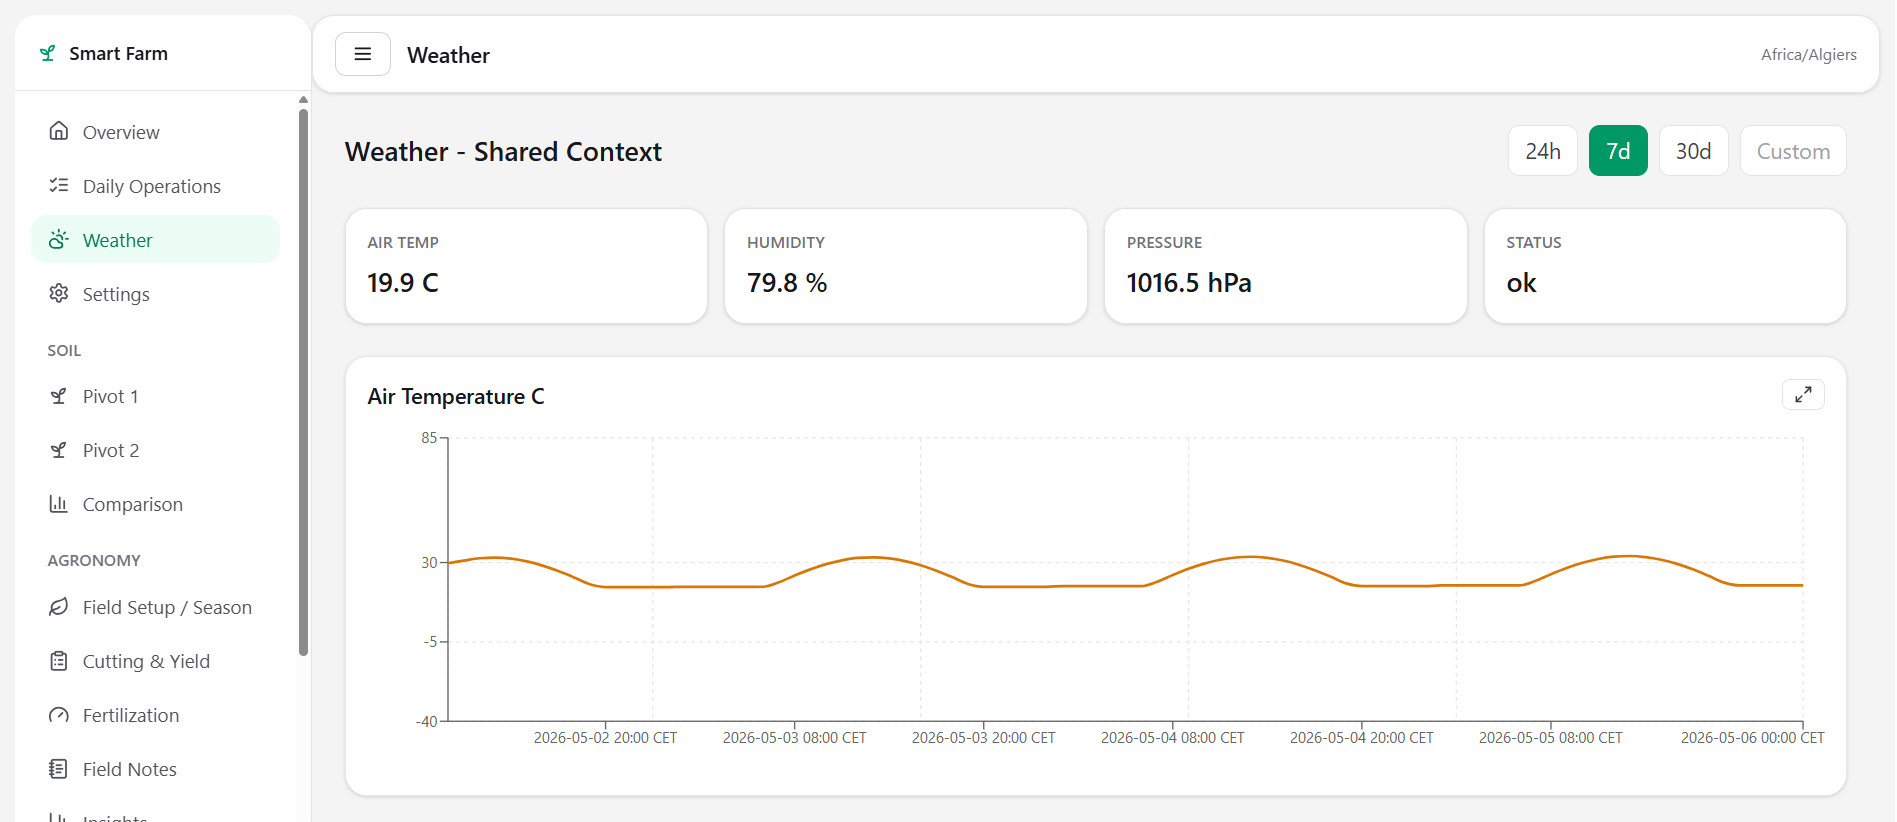
\includegraphics[width=\textwidth]{figures/DashWeather}
% TODO: copy Academic-Thesis/DashBoredImages/Weather.png to figures/DashWeather.png before compiling
\caption{Weather monitoring page presenting air temperature, relative humidity, and barometric pressure time series from Node3.}
\label{fig:weather-dashboard}
\end{figure}

The weather page displays the three atmospheric parameters provided by Node3: air temperature, relative humidity, and barometric pressure. These measurements provide agronomic context for interpreting soil moisture trends and are presented on the same measurement-time axis as the soil charts, preserving temporal alignment across the monitoring domains.

\begin{figure}[H]
\centering
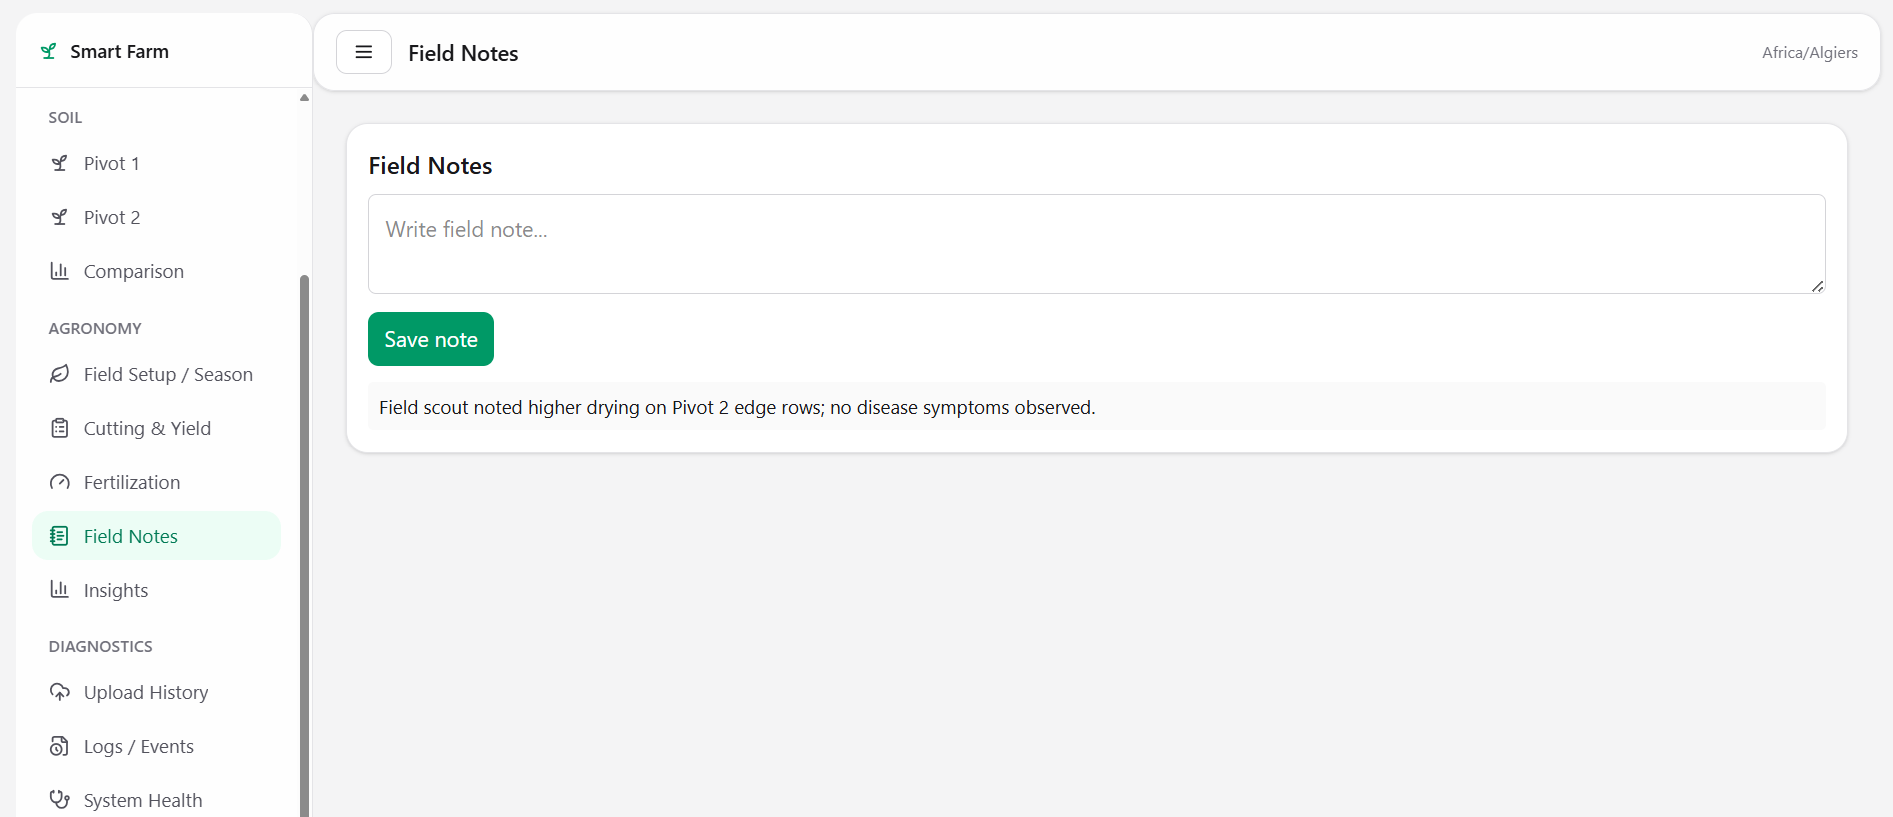
\includegraphics[width=\textwidth]{figures/DashFieldNotes}
% TODO: copy Academic-Thesis/DashBoredImages/FieldNotes.png to figures/DashFieldNotes.png before compiling
\caption{Field notes and agronomic events page listing manually recorded irrigation sessions, fertilisation applications, and field observations, with start and end times stored in the \texttt{agronomic\_events} table.}
\label{fig:field-notes-dashboard}
\end{figure}

The field notes page presents the \texttt{agronomic\_events} table in a chronological list, exposing operator-entered records of irrigation sessions, fertilisation applications, and field observations. These records are stored independently of the sensor reading domain and are overlaid on soil moisture charts to provide interpretive context. The interface does not interpret or annotate agronomic events automatically; the operator supplies all semantic meaning through the event type and notes fields at the time of entry.

% ============================================================
\section{Deterministic Analytics Layer}
\label{sec:analytics}
% ============================================================

The deterministic analytics layer is the computational engine of the platform. It operates on uploaded sensor readings to produce quality-controlled, reliability-scored, and alert-evaluated outputs that are stored as analytics snapshots and presented to the operator through the Insights and Processed Data Viewer pages. The layer is deterministic: given the same input readings, quality flags, and configured thresholds, it produces the same output every time. Gemini does not participate in any stage of this pipeline; AI-generated narratives are prepared only after the deterministic outputs have been computed and stored.

\begin{figure}[H]
\centering
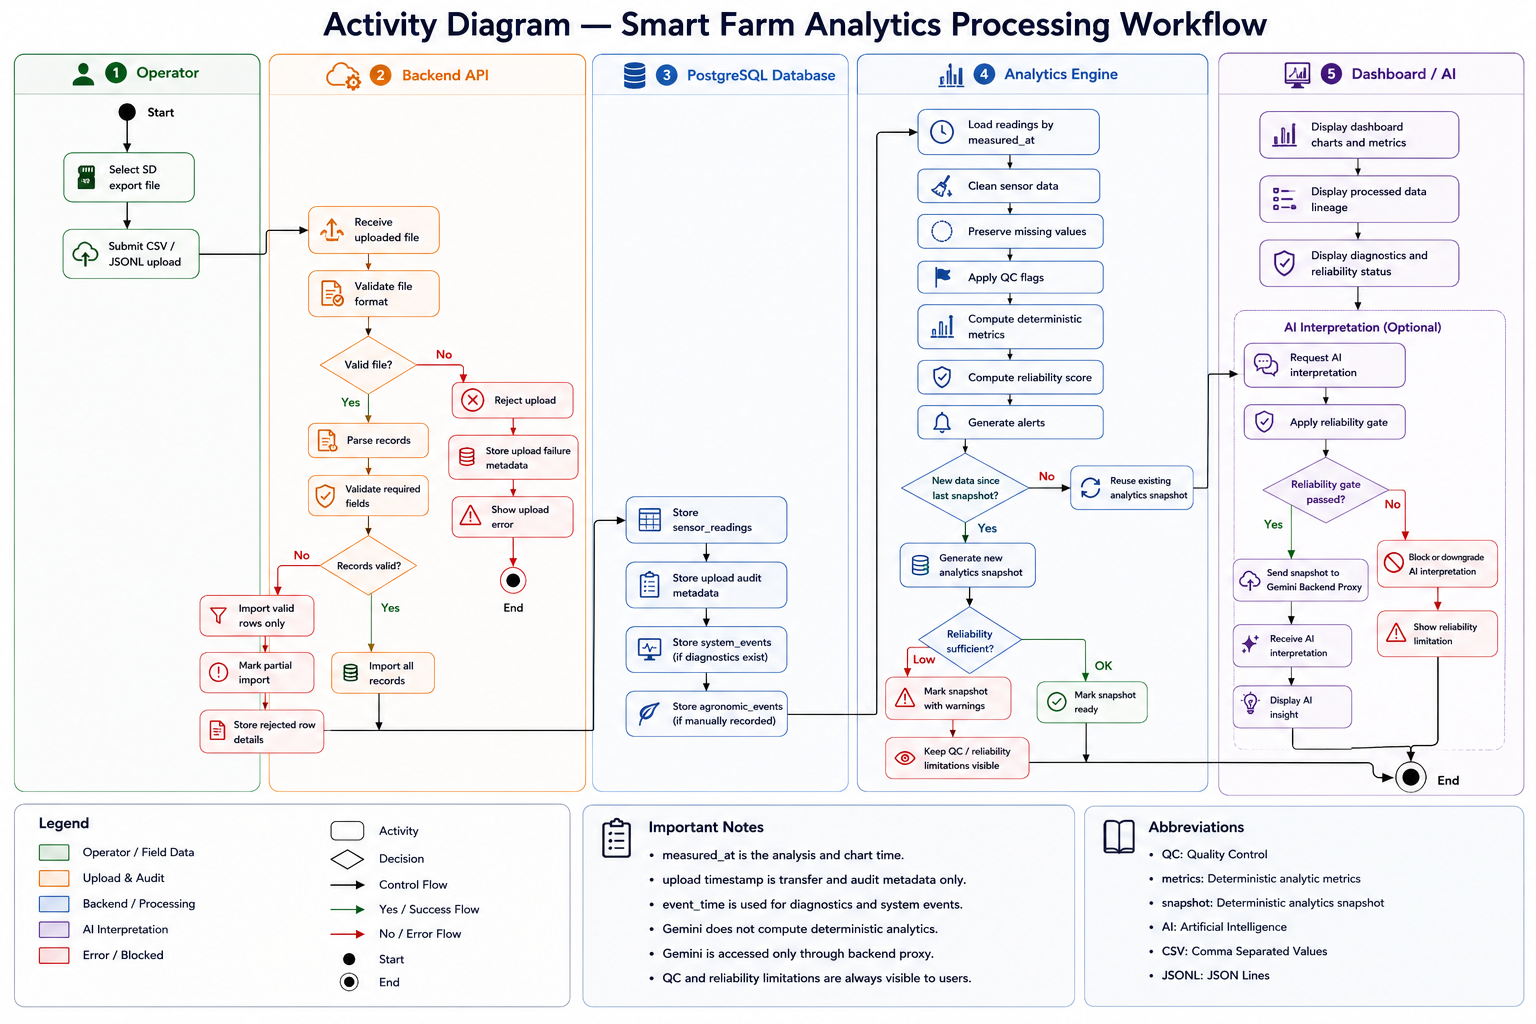
\includegraphics[width=0.90\textwidth]{figures/ActivityDiagram}
% TODO: copy Academic-Thesis/Diagrams/Activity Diagram.png to figures/ActivityDiagram.png before compiling
\caption{Activity diagram of the deterministic analytics pipeline, showing the sequence from raw sensor readings through timestamp validation, duplicate detection, range and flatline checking, quality scoring, reliability scoring, alert evaluation, and analytics snapshot generation.}
\label{fig:deterministic-analytics-workflow}
\end{figure}

The pipeline proceeds through ten ordered stages. Raw sensor readings enter from the \texttt{sensor\_readings} table. Each stage applies a rule set and passes annotated records to the next stage; no stage modifies the stored sensor values — quality flags and derived metrics are maintained separately. Table~\ref{tab:analytics-pipeline} describes each stage in detail.

\begin{table}[H]
\centering
\caption{Stages of the deterministic analytics pipeline, showing inputs, processing roles, outputs, and safety boundaries at each stage.}
\label{tab:analytics-pipeline}
\small
\begin{tabular}{p{2.8cm} p{2.5cm} p{3.0cm} p{2.8cm} p{2.5cm}}
\hline
\textbf{Stage} & \textbf{Input} & \textbf{Processing role} & \textbf{Output} & \textbf{Safety boundary} \\
\hline
Canonical timestamp check & Raw readings & Verify \texttt{measured\_at} is present and in UTC; normalise timezone representation & Timestamp-validated set & Records without \texttt{measured\_at} are excluded, not corrected \\
\hline
Duplicate detection & Timestamp-validated set & Identify records sharing the same node and \texttt{measured\_at} within tolerance & Deduplicated set with duplicate flags & Originals preserved; duplicates flagged, not deleted \\
\hline
Missing data analysis & Deduplicated set & Count and characterise gaps per measurement window & Gap map per node and domain & Values are never imputed; gaps remain visible \\
\hline
Physical range checking & Sensor readings & Compare values against physical bounds for each measurement type & Range-flagged annotations & No automatic value correction; operator-visible flag only \\
\hline
Flatline and spike detection & Range-checked readings & Statistical consistency checks across consecutive readings & Quality-flagged annotations & Suspect readings remain in the dataset with flags; not silently removed \\
\hline
System-event cross-reference & Quality flags + system events & Align diagnostic events with the measurement window & Event-aligned quality annotations & Does not override QC flags; adds context only \\
\hline
Window quality scoring & Quality flags + agronomic event confidence & Compute a weighted quality metric per time window & Window quality score & Agronomic event confidence weighting is additive; does not suppress low-quality flags \\
\hline
Node reliability scoring & Window quality scores + upload metadata & Aggregate per-node reliability across the analysis window & Node reliability indicator & Upload freshness affects score; low reliability remains exposed, not normalised \\
\hline
Deterministic alert evaluation & Reliability score + quality flags & Evaluate configured threshold conditions & Alert records & No AI involvement; thresholds are operator-configured values \\
\hline
Analytics snapshot & All stage outputs & Aggregate quality score, reliability, alerts, and limitations into a \texttt{analytics\_snapshots} record & Snapshot stored in PostgreSQL & This snapshot — not raw data — is the only input forwarded to the Gemini proxy \\
\hline
\end{tabular}
\end{table}

Two additional inputs feed into the quality and reliability stages. Agronomic events recorded in the \texttt{agronomic\_events} table contribute a confidence weight to the window quality scoring stage, reflecting the principle that a window accompanied by a recorded irrigation or fertilisation event carries stronger interpretive context. Upload metadata from the \texttt{uploads} table informs the upload freshness diagnostic component of node reliability scoring.

\begin{figure}[H]
\centering
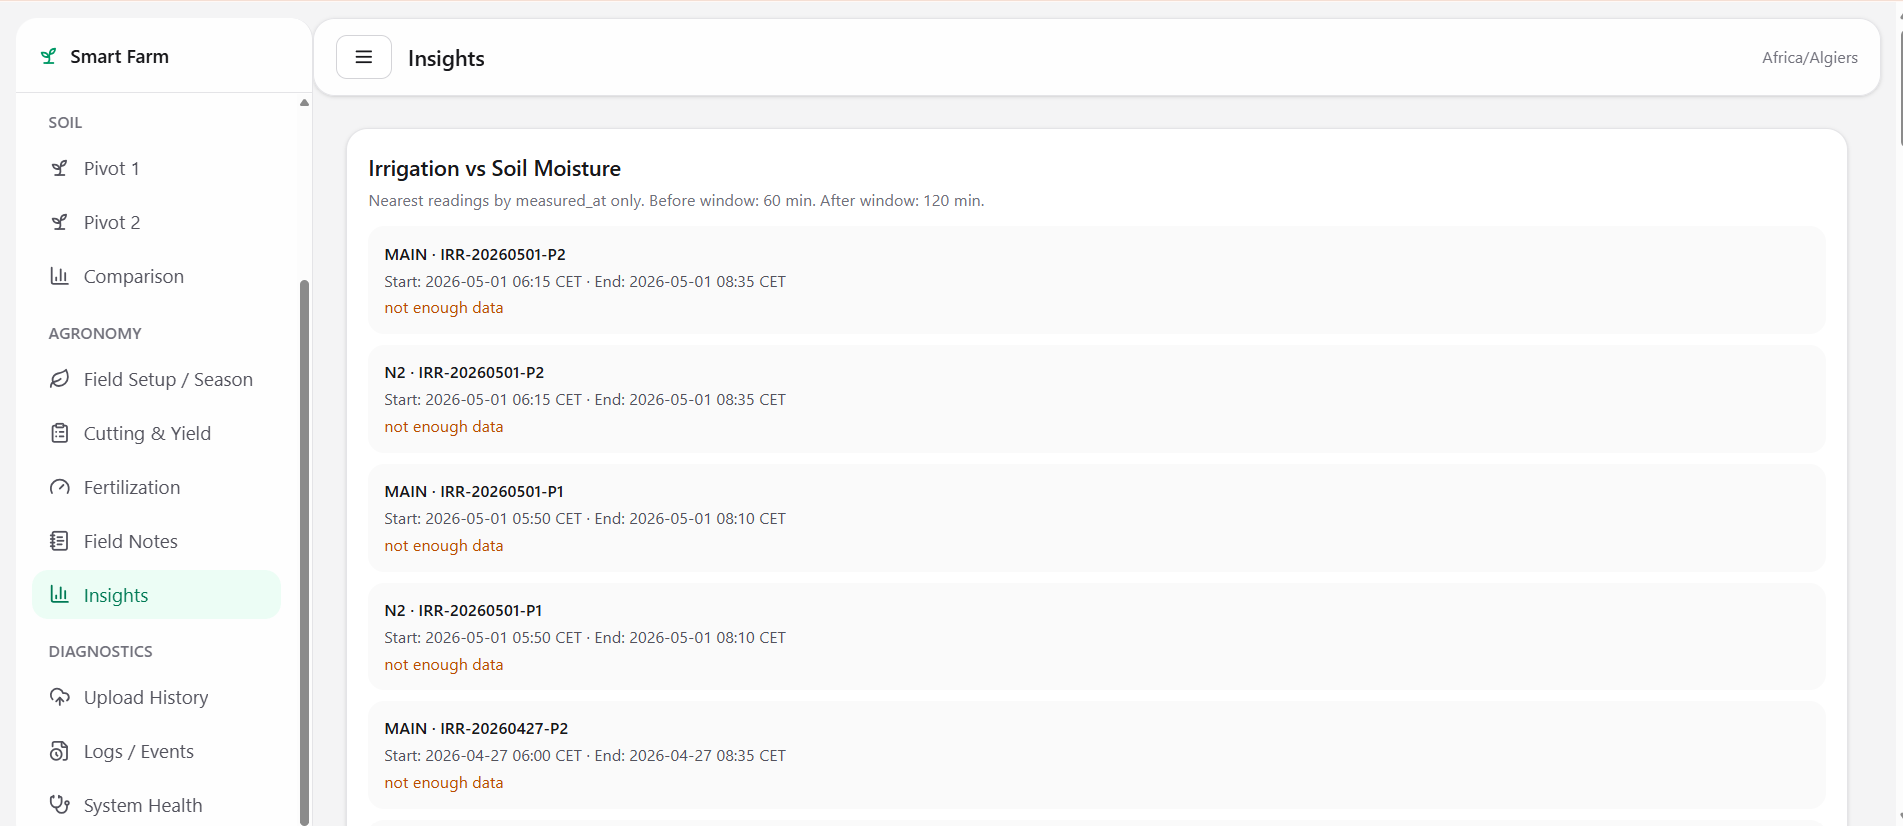
\includegraphics[width=\textwidth]{figures/DashInsights}
% TODO: copy Academic-Thesis/DashBoredImages/Insights.png to figures/DashInsights.png before compiling
\caption{Analytics Insights page displaying deterministic quality scores, reliability indicators, and alert summaries derived from the analytics pipeline. AI-generated narratives appear in a separate, clearly labelled panel.}
\label{fig:insights-dashboard}
\end{figure}

The Insights page presents the outputs of the deterministic pipeline alongside any AI-generated narrative that has been requested for the current analytics snapshot. The deterministic metrics — quality score, reliability indicator, and alert list — are displayed in the primary panel. The AI narrative appears in a secondary panel with a visual label identifying it as an AI-generated interpretation. The physical separation reinforces the principle that deterministic analytics are the authoritative layer and AI narratives are supplementary decision-support information.

% ============================================================
\section{Processed Data Viewer}
\label{sec:processed-data-viewer}
% ============================================================

The Processed Data Viewer is a read-only transparency interface that exposes the full output of the deterministic analytics pipeline for a selected time window. Its purpose is to allow the operator — and, in an academic context, the reviewer — to inspect the lineage from raw sensor readings through each processing stage to the final quality-annotated result.

\begin{figure}[H]
\centering
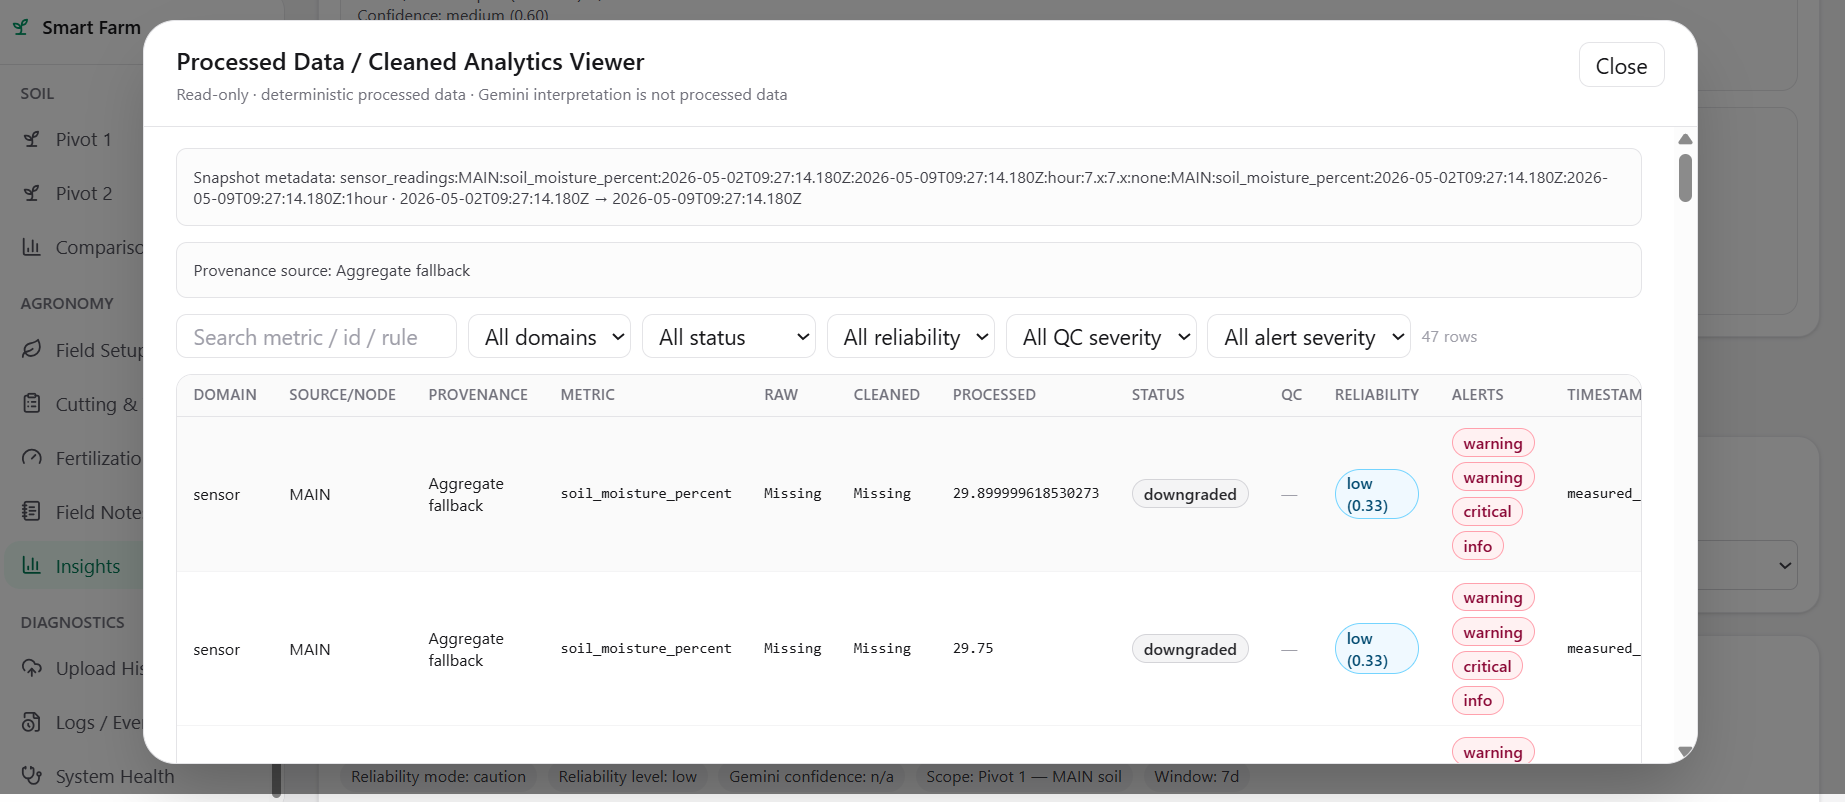
\includegraphics[width=\textwidth]{figures/ProcessedData}
% TODO: The source file is Academic-Thesis/DashBoredImages/ProcessedData .png — note the space before the extension. Rename to ProcessedData.png before copying to figures/ProcessedData.png, or escape the space in the LaTeX path if the toolchain supports it.
\caption{Processed Data Viewer page showing the output of the deterministic analytics pipeline for the selected analysis window, including per-record quality flags, reliability indicator, deterministic alert references, and a safe export function.}
\label{fig:processed-data-viewer}
\end{figure}

The viewer presents the output of the \texttt{analytics\_snapshots} table for the selected window. For each processed record, it exposes the raw input values, the quality flags applied at each pipeline stage, the window quality score, the node reliability indicator, any deterministic alerts that were triggered, and any limitations attached to the record. The viewer does not expose an editing interface; all values are read-only, and the raw sensor readings in the \texttt{sensor\_readings} table are not modified by the analytics pipeline at any stage.

A safe export function allows the operator to download the processed data in a portable format for offline analysis or academic reporting. The exported file includes the processing lineage columns alongside the sensor values, preserving the full context needed to reproduce the quality assessment independently.

% ============================================================
\section{AI Interpretation Layer}
\label{sec:ai-interpretation}
% ============================================================

The AI interpretation layer provides narrative context to support operator decision-making. It is implemented as a backend-proxied interface to the Gemini generative AI model. The layer is deliberately constrained: it operates downstream of the deterministic analytics pipeline, receives only the processed analytics snapshot, and produces narrative text that is presented to the operator alongside — not in place of — the deterministic outputs.

\begin{figure}[H]
\centering
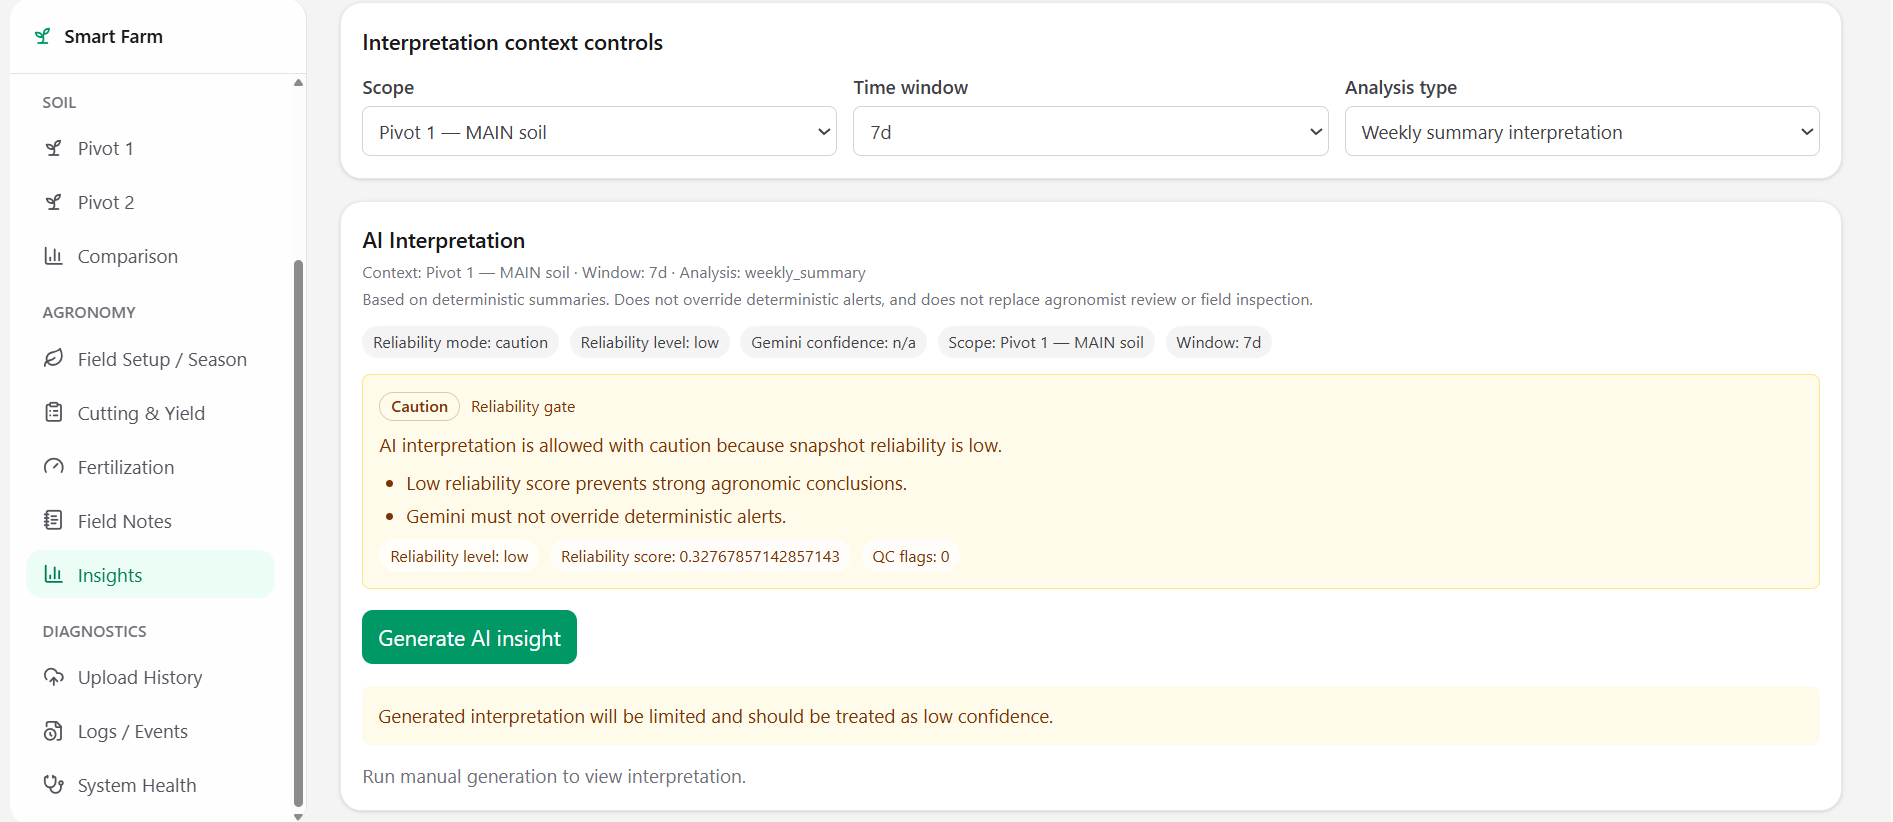
\includegraphics[width=\textwidth]{figures/DashAiInsight}
% TODO: copy Academic-Thesis/DashBoredImages/AiInsight.png to figures/DashAiInsight.png before compiling
\caption{AI Insight page presenting a Gemini-generated narrative interpretation of the current analytics snapshot. The deterministic metrics, reliability indicator, and QC flags are passed as context; the AI response is labelled as an interpretive narrative and presented separately from the deterministic layer.}
\label{fig:ai-interpretation-ui}
\end{figure}

The boundary governing the AI layer is defined at six levels, described in Table~\ref{tab:ai-boundary}. Each boundary addresses a specific risk: data integrity, metric reproducibility, scope control, user misinterpretation, and the agronomist principle established in Chapter~\ref{chap:related-works}.

\begin{table}[H]
\centering
\caption{AI interpretation boundary rules, their implementation, and rationale.}
\label{tab:ai-boundary}
\small
\begin{tabular}{p{3.5cm} p{5.0cm} p{5.0cm}}
\hline
\textbf{Boundary rule} & \textbf{Implementation meaning} & \textbf{Reason} \\
\hline
Backend proxy only & Gemini API calls are routed exclusively through the WebService backend; the dashboard frontend never calls the Gemini API directly & Prevents raw sensor data, database content, and API credentials from being exposed at the client layer \\
\hline
Snapshot input only & Gemini receives the deterministic analytics snapshot; it does not receive raw \texttt{sensor\_readings} rows, individual reading objects, or direct database query results & Constrains AI interpretation scope to validated, quality-annotated output rather than unprocessed measurements \\
\hline
No raw data mutation & Gemini cannot write to the database, modify reading values, fill missing values, alter QC flags, or change alert severity & Preserves the integrity of the sensor record and the reproducibility of the deterministic pipeline \\
\hline
No metric computation & Quality scores, reliability indicator, and alert evaluation are computed deterministically before Gemini is invoked; Gemini is not asked to recompute or validate any metric & Ensures primary analytics are reproducible from project code, not dependent on AI model state \\
\hline
Reliability gate & A reliability threshold check is applied before the snapshot is forwarded; a low-confidence snapshot triggers an operator-visible warning before AI interpretation is requested & Prevents AI narrative from appearing normal when underlying data quality is insufficient \\
\hline
Human decision final & AI-generated narratives are presented as decision-support information; agronomic decisions remain with the human operator & Consistent with the monitoring-only scope of the system and the agronomist boundary established in Section~\ref{sec:proposed-improvements} \\
\hline
\end{tabular}
\end{table}

The \texttt{/api/v1/gemini} endpoint enforces all six boundaries in a single processing function. The function retrieves the analytics snapshot, evaluates the reliability gate, constructs a structured prompt containing the snapshot context and the system's declared constraints, forwards the prompt to the Gemini API, and returns the narrative response to the dashboard. The response is never stored in the \texttt{sensor\_readings}, \texttt{system\_events}, or \texttt{analytics\_snapshots} tables; it exists only as a transient response for the current session.

% ============================================================
\section{Field Deployment}
\label{sec:deployment}
% ============================================================

The system was assembled and deployed as a field-oriented prototype for monitoring alfalfa cultivation in the El~Oued region of Algeria. The deployment context is consistent with the Saharan agricultural environment described in Section~\ref{sec:saharan-agriculture}: intermittent power availability, no permanent Internet connection at the field site, and a need for autonomous data acquisition across multi-day periods between operator visits.

The three nodes described in Section~\ref{sec:hardware} were mounted and positioned according to their sensing roles. The MAIN gateway was installed at the Pivot~1 location, providing both LoRa reception coordination and local soil monitoring for the first irrigation zone. Node2 was deployed at the Pivot~2 location, independently acquiring soil measurements for the second irrigation zone and transmitting them to MAIN over LoRa. Node3 was positioned as a dedicated weather station, collecting atmospheric parameters over the full deployment window.

Node operation during the deployment follows the manual workflows described in Sections~\ref{sec:mode-upload} and~\ref{sec:mode-rtc-sync}. The operator visits the field site with an Internet connection periodically, connects the MAIN node to the available network, and activates Upload Mode with a sustained button press to transfer accumulated SD content to the backend. RTC synchronisation is performed with four consecutive button presses before the upload session if clock drift is suspected. Between operator visits, the three nodes cycle through the ten-minute superframe independently, storing measurements locally on the MAIN SD card without any network dependency.

The three nodes were housed in protective enclosures rated IP65, providing resistance to dust ingress and water contact from all directions. In the Saharan field context, this rating addresses the primary environmental risks to embedded electronics: wind-borne fine sand and dust, periodic humidity, and incidental mechanical contact during maintenance visits. The IP65 rating does not imply submersion tolerance; the nodes are not waterproof to immersion. Figures~\ref{fig:field-main-node-deployment}, \ref{fig:field-node2-soil-enclosure}, and~\ref{fig:field-node3-weather-enclosure} document the three deployed nodes in their respective field positions.

\begin{figure}[H]
\centering
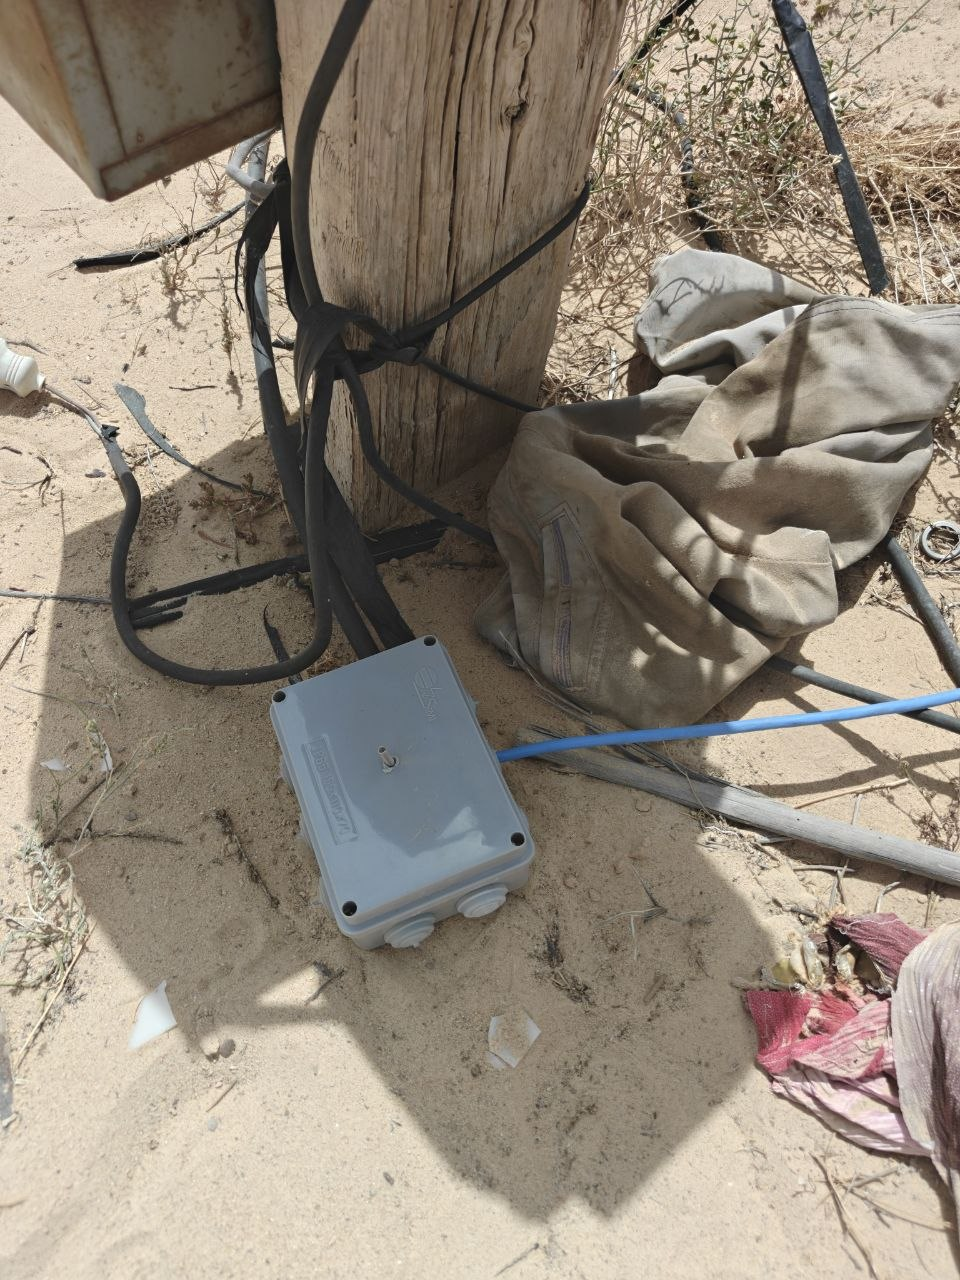
\includegraphics[width=0.72\textwidth]{figures/field-main-node-deployment}
\caption{MAIN gateway node at the Pivot~1 field location during the pilot deployment. The IP65-rated enclosure provides dust and water-contact resistance appropriate for outdoor Saharan field conditions. The node operates on battery power. Electrical infrastructure visible in the surrounding area belongs to the existing field site; it does not serve as the node power source.}
\label{fig:field-main-node-deployment}
\end{figure}

\begin{figure}[H]
\centering
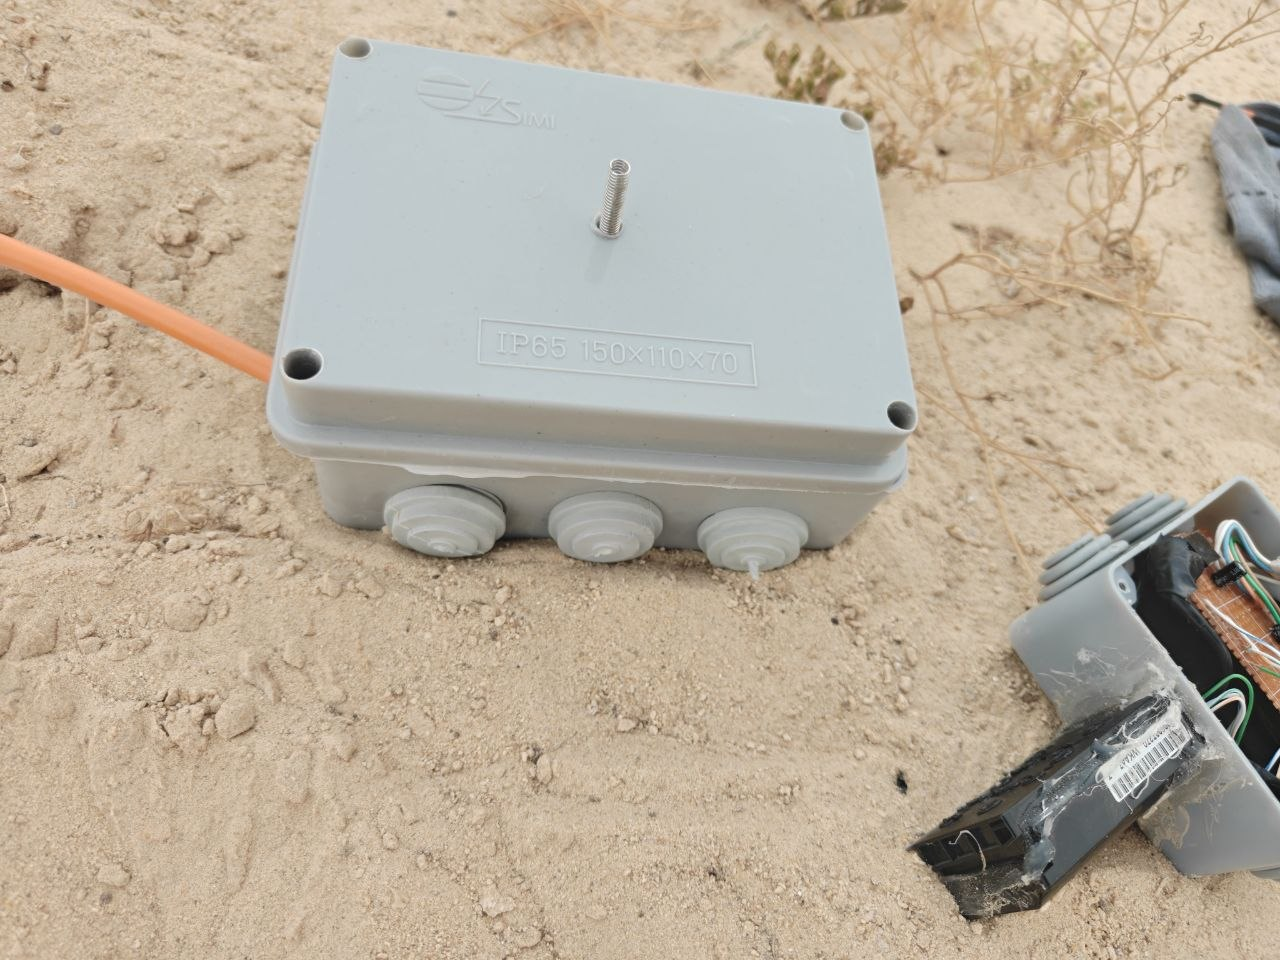
\includegraphics[width=0.72\textwidth]{figures/field-node2-soil-enclosure}
\caption{Node2 soil sensing enclosure at the Pivot~2 field location. A CAT6 RJ45 outdoor cable connects the enclosure to the in-ground RS485 soil sensor, carrying the sensor signal and power conductors required by the Modbus soil sensing interface. The cable was selected for its outdoor insulation, humidity and soil-contact resistance, reliable copper conductors, and multi-conductor configuration; it functions as a utility signal cable in this application, not as an Ethernet connection.}
\label{fig:field-node2-soil-enclosure}
\end{figure}

\begin{figure}[H]
\centering
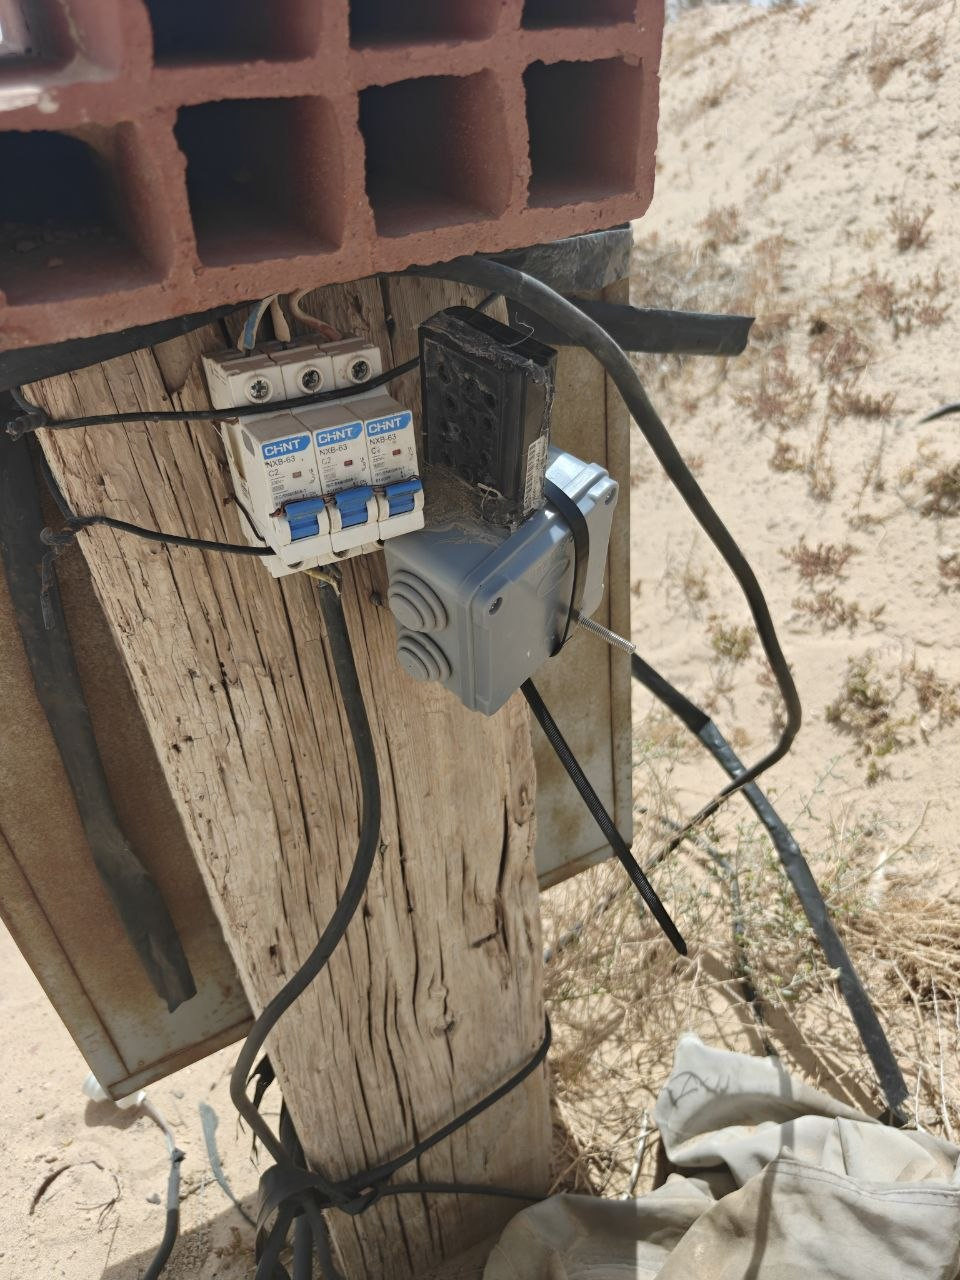
\includegraphics[width=0.72\textwidth]{figures/field-node3-weather-enclosure}
\caption{Node3 weather sensing node at its field position during the pilot validation window. The IP65-rated enclosure houses the ESP32-C3, LoRa transceiver, and BME280 sensor, providing dust and water-contact protection suitable for outdoor atmospheric monitoring in a Saharan environment.}
\label{fig:field-node3-weather-enclosure}
\end{figure}

The deployment does not constitute a formal long-term field trial. The evidence presented in this chapter spans a 5.5-day validation window from 2026-05-06 to 2026-05-11, during which the system operated across six upload sessions. This window demonstrates functional feasibility and the end-to-end operation of the sensing, storage, upload, and analytics pipeline. Long-term robustness, seasonal measurement coverage, and calibrated agronomic threshold validation are identified as future work in Section~\ref{sec:limitations}.

% ============================================================
\section{Data Analysis and Results}
\label{sec:results}
% ============================================================

The data presented in this section were acquired during the pilot validation window from 2026-05-06 00:00~UTC to 2026-05-11 15:00~UTC. All measurements originate from the sensor nodes and were transferred to the backend across six upload sessions. The analysis is bounded by the available evidence and is intended to demonstrate functional feasibility of the data acquisition, storage, transfer, and processing pipeline — not to draw calibrated agronomic conclusions.

\begin{table}[H]
\centering
\caption{Summary of validation dataset evidence, observed values, and interpretation scope.}
\label{tab:validation-data-summary}
\small
\begin{tabular}{p{3.5cm} p{3.5cm} p{6.5cm}}
\hline
\textbf{Evidence item} & \textbf{Value} & \textbf{Interpretation} \\
\hline
Sensor readings & 2433 total & 811 records per node (MAIN, N2, N3); equal distribution confirms superframe-level consistency across the validation window \\
\hline
Missing \texttt{measured\_at} & 0 rows & Every reading carries a canonical measurement timestamp; timestamp policy enforced at ingestion \\
\hline
Reading status & All \texttt{ok} & No ingestion-level rejection within the provided dataset; status reflects database record state \\
\hline
System events & 8 & Logged from 2026-05-08 to 2026-05-11; include node-missing events, an irrigation-completed record, and a heat-stress warning \\
\hline
Agronomic events & 6 & Four irrigation sessions (Pivot~1 and Pivot~2 on 2026-05-08 and 2026-05-11), one fertilisation application (2026-05-10), one field scouting note (2026-05-09) \\
\hline
Upload sessions & 6 & All sessions reached \texttt{processed} status; three upload anomalies recorded in one session \\
\hline
Processed data rows & 135 & Output of the deterministic analytics pipeline for the analysis window; reliability indicator uniform at 0.399 across all rows \\
\hline
Validation window & 5 days 15 hours & Pilot validation window; functional feasibility scope only — not full-season agronomic validation \\
\hline
\end{tabular}
\end{table}

Table~\ref{tab:node-data-summary} provides a per-node breakdown of the sensor records, including the received signal strength indicators that document the LoRa link quality over the validation period.

\begin{table}[H]
\centering
\caption{Per-node record summary for the validation window, showing measurement types, record counts, and observed LoRa signal quality indicators.}
\label{tab:node-data-summary}
\small
\begin{tabular}{p{1.5cm} p{3.0cm} p{1.5cm} p{3.0cm} p{4.5cm}}
\hline
\textbf{Node} & \textbf{Role} & \textbf{Records} & \textbf{Measurement types} & \textbf{Signal quality and notes} \\
\hline
MAIN & Gateway + Pivot~1 local soil (register map pending) & 811 & Gateway-level records; Pivot~1 soil path active, register map confirmation required & Avg RSSI: $-85.4$~dBm; Avg SNR: 8.5~dB; Pivot~1 soil values require register map resolution \\
\hline
N2 & Pivot~2 remote soil node & 811 & Soil moisture (\%), temperature (°C), EC (µS/cm) & Avg RSSI: $-97.0$~dBm; Avg SNR: 6.1~dB; longest LoRa path; consistent reception \\
\hline
N3 & Weather station & 811 & Air temperature (°C), humidity (\%), pressure (hPa) & Avg RSSI: $-76.4$~dBm; Avg SNR: 9.6~dB; strongest signal; nearest deployment position \\
\hline
\end{tabular}
\end{table}

The equal record count of 811 per node across the 5.5-day window is consistent with a ten-minute superframe cycle producing six readings per hour. The distribution confirms that all three nodes transmitted and that the MAIN gateway received and stored data for each node throughout the validation period, with no multi-hour gaps in any node's record.

The N2 node provides the primary soil monitoring data for Pivot~2. Soil moisture, temperature, and EC readings from N2 form the principal time series for irrigation-response analysis. The agronomic events recorded during the validation window — two irrigation sessions on 2026-05-08 and two on 2026-05-11, together with a fertilisation application on 2026-05-10 and a heat-stress field observation on 2026-05-09 — provide the interpretive context for examining N2 soil data trends. Without sensor calibration data, these trends are evaluated as relative patterns rather than absolute agronomic thresholds.

The N3 weather node delivered atmospheric readings across the full window, providing air temperature, humidity, and pressure context for the same period. The field scouting note of 2026-05-09 identifying heat-stress risk is consistent with the atmospheric monitoring purpose of Node3: elevated air temperature and reduced humidity readings around that date provide the measurement context for a heat-stress advisory, even if the advisory itself was recorded manually rather than computed automatically.

The deterministic analytics pipeline produced 135 processed rows from the analysis window. A uniform reliability indicator of 0.399 was computed for all rows. This value is a pilot-phase indicator produced by the pipeline's initial configuration; it does not represent a calibrated or field-validated reliability threshold. Section~\ref{sec:limitations} addresses the calibration requirement explicitly.

% ============================================================
\section{Validation and Testing}
\label{sec:validation}
% ============================================================

Validation of the system covers seven functional categories corresponding to the major design components: hardware assembly, LoRa communication, local storage, upload and backend ingestion, dashboard rendering, deterministic analytics, and the AI interpretation boundary. Evidence for each category is drawn from the validation package described in Section~\ref{sec:results}.

\begin{figure}[H]
\centering
\begin{minipage}[b]{0.48\textwidth}
\centering
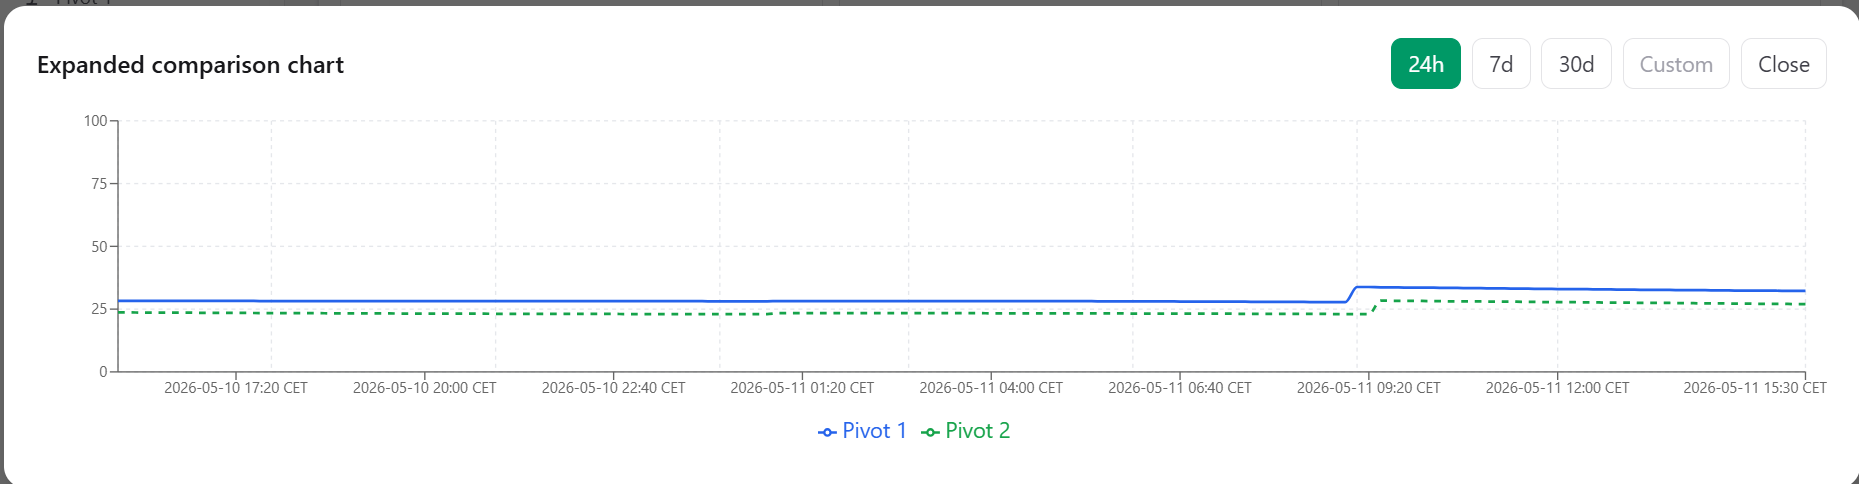
\includegraphics[width=\textwidth]{figures/val-pivot-comparison-24h}
% TODO: copy Academic-Thesis/validation_package/02_validation_evidence/dashboard_screenshots/01_pivot_comparison_expanded_24h.png to figures/val-pivot-comparison-24h.png before compiling
\caption{Dashboard pivot comparison chart expanded to a 24-hour view, demonstrating time-aligned soil monitoring across two irrigation zones.}
\label{fig:validation-pivot-comparison-24h}
\end{minipage}
\hfill
\begin{minipage}[b]{0.48\textwidth}
\centering
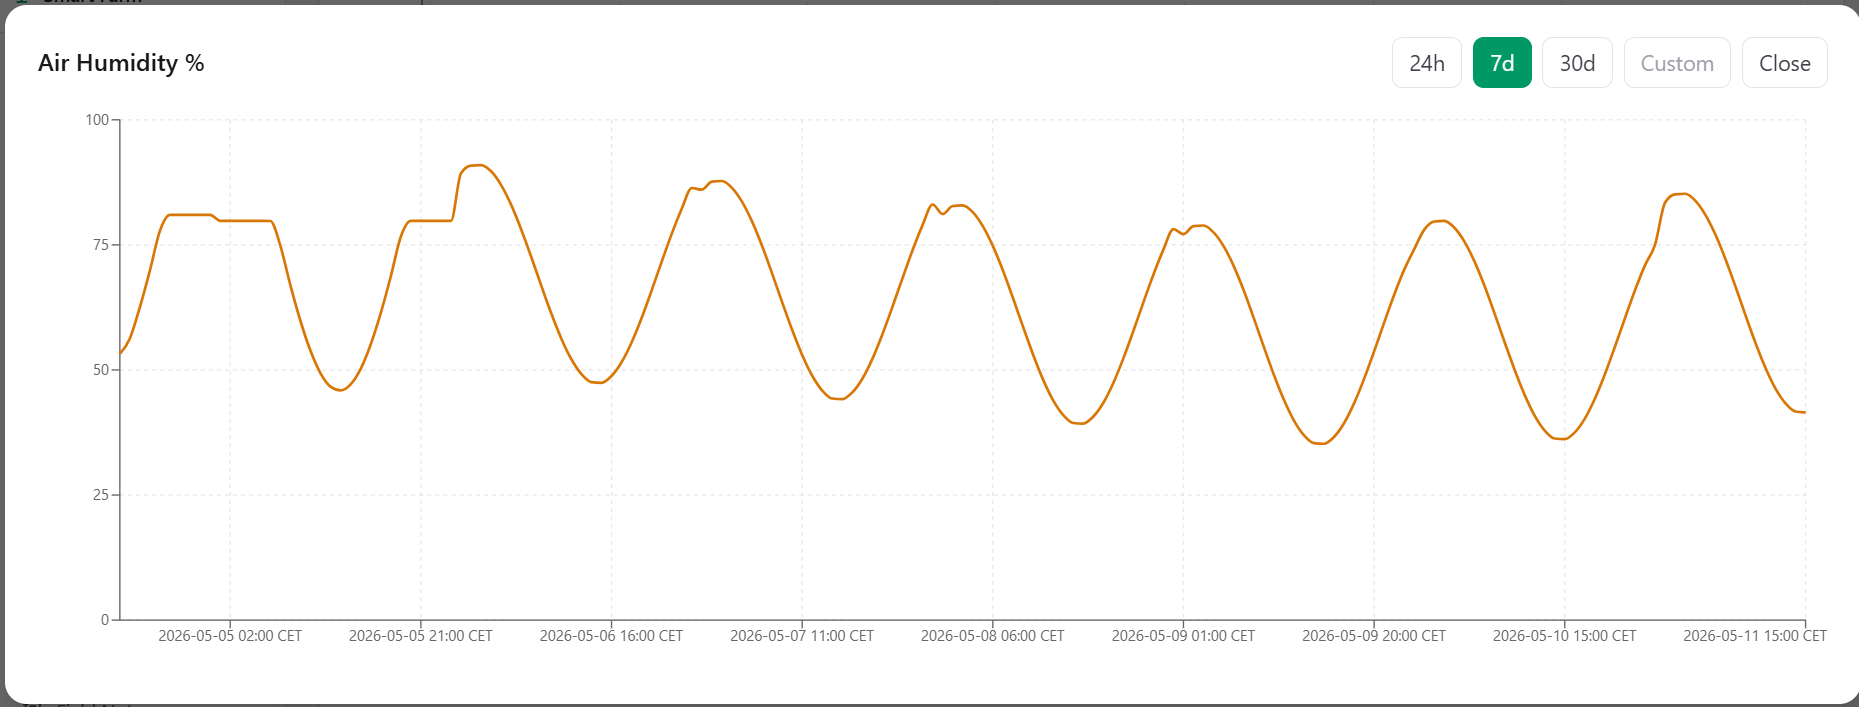
\includegraphics[width=\textwidth]{figures/val-weather-humidity-7d}
% TODO: copy Academic-Thesis/validation_package/02_validation_evidence/dashboard_screenshots/02_weather_air_humidity_7d.png to figures/val-weather-humidity-7d.png before compiling
\caption{Dashboard weather page showing the 7-day air humidity trend from Node3 over the validation window.}
\label{fig:validation-weather-humidity-7d}
\end{minipage}
\end{figure}

\begin{figure}[H]
\centering
\begin{minipage}[b]{0.48\textwidth}
\centering
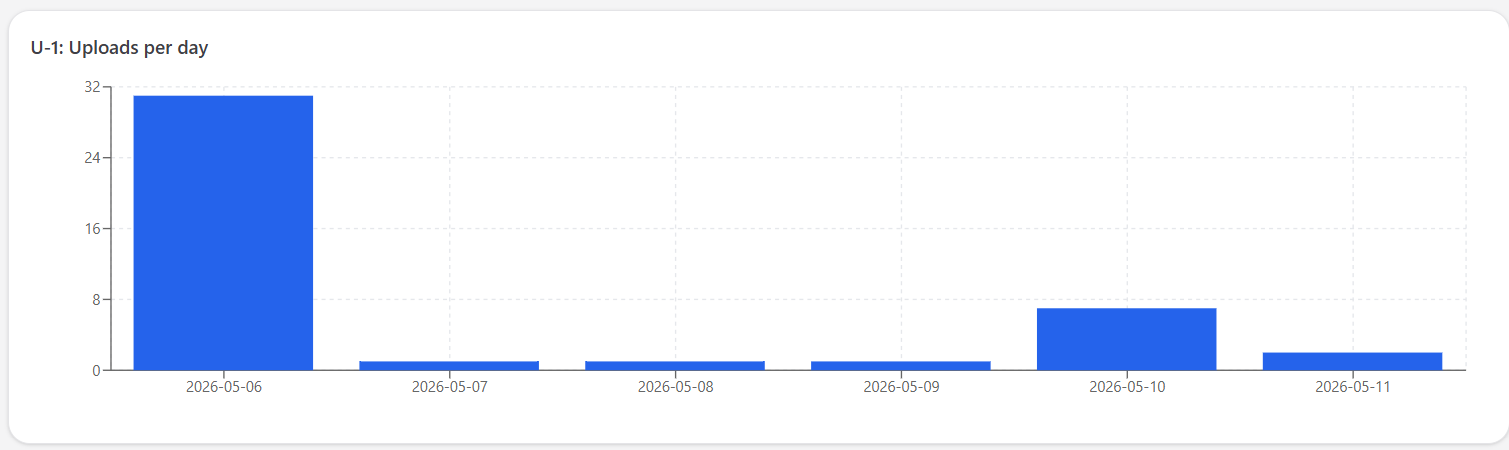
\includegraphics[width=\textwidth]{figures/val-uploads-per-day}
% TODO: copy Academic-Thesis/validation_package/02_validation_evidence/dashboard_screenshots/03_uploads_per_day.png to figures/val-uploads-per-day.png before compiling
\caption{Dashboard upload history view showing daily upload sessions across the validation window. Six sessions are shown, all with processed status.}
\label{fig:validation-uploads-per-day}
\end{minipage}
\hfill
\begin{minipage}[b]{0.48\textwidth}
\centering
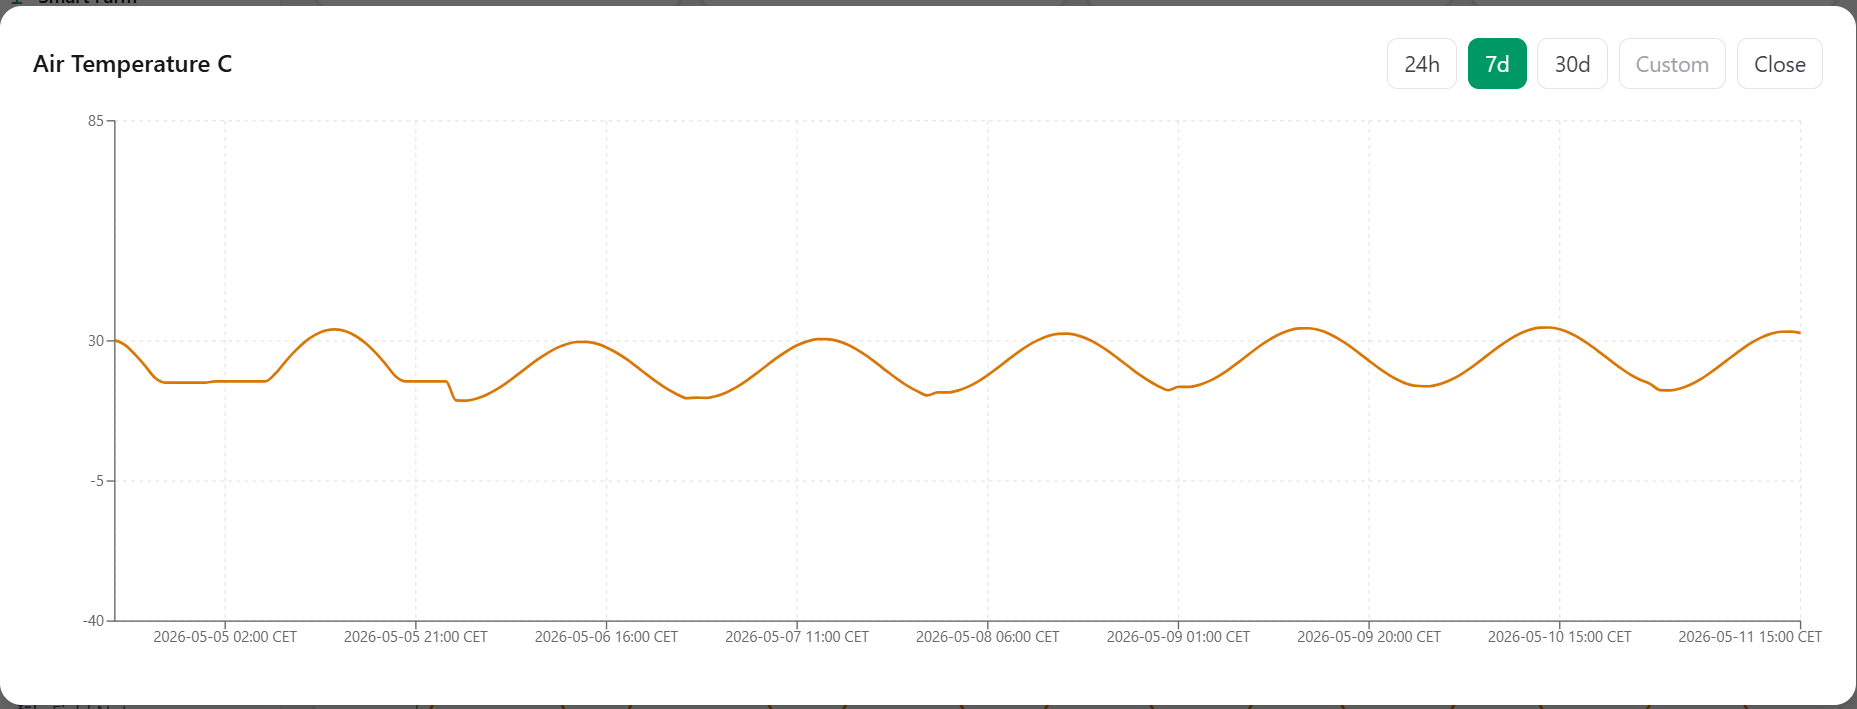
\includegraphics[width=\textwidth]{figures/val-weather-temperature-7d}
% TODO: copy Academic-Thesis/validation_package/02_validation_evidence/dashboard_screenshots/04_weather_air_temperature_7d.png to figures/val-weather-temperature-7d.png before compiling
\caption{Dashboard weather page showing the 7-day air temperature trend from Node3, providing atmospheric context for the agronomic event timeline.}
\label{fig:validation-weather-temperature-7d}
\end{minipage}
\end{figure}

Table~\ref{tab:validation-tests} consolidates the seven validation categories with their evidence sources, observed results, and acknowledged limitations.

\begin{table}[H]
\centering
\caption{Validation test summary by functional category, showing evidence used, observed results, and known limitations.}
\label{tab:validation-tests}
\small
\begin{tabular}{p{2.5cm} p{3.0cm} p{4.0cm} p{4.0cm}}
\hline
\textbf{Test area} & \textbf{Evidence used} & \textbf{Observed result} & \textbf{Limitation} \\
\hline
Hardware assembly & Node photos (Figures~\ref{fig:main-node-front}–\ref{fig:node3-back}); wiring diagrams & Three-node system assembled and documented; all subsystems present per wiring diagrams & Physical stress, temperature, and vibration tolerance not formally assessed \\
\hline
LoRa communication & Firmware serial transcript; RSSI/SNR values in sensor readings CSV & LoRa packet reception confirmed for all three nodes; RSSI range $-76$ to $-97$~dBm; ACK behaviour documented in serial log & Formal range characterisation over measured field distances not conducted \\
\hline
Local storage & Firmware serial transcript; upload queue JSONL file & SD write operations confirmed per measurement cycle in serial log; JSONL upload queue present and non-empty & SD card capacity limits and long-term write endurance not evaluated \\
\hline
Upload and backend ingestion & Uploads CSV (6 sessions, all \texttt{processed}); readings count match (2433 uploaded = 2433 in \texttt{sensor\_readings}) & All six sessions reached processed status; three upload anomalies recorded in one session; ingested record count matches upload row count & API response samples not captured; build terminal output not available \\
\hline
Dashboard rendering & Four validation screenshots (Figures~\ref{fig:validation-pivot-comparison-24h}–\ref{fig:validation-weather-temperature-7d}) & Pivot comparison, weather, and upload history charts rendered with data from the validation window & Full UI test coverage not conducted; page load time and browser compatibility not formally measured \\
\hline
Deterministic analytics and QC & Processed data CSV (135 rows); analytics structure & Pipeline produced quality-annotated output for the analysis window; reliability indicator computed for all rows & Reliability threshold calibration not completed; alert threshold tuning not documented in this validation window \\
\hline
AI interpretation boundary & Architecture design; backend proxy code structure; \texttt{/api/v1/gemini} endpoint scope & Gemini receives analytics snapshot only; frontend never calls Gemini directly; reliability gate confirmed in endpoint logic & Boundary validation is a design and architecture review; live adversarial testing not conducted \\
\hline
\end{tabular}
\end{table}

The firmware serial transcript confirms the packet reception sequence described in Section~\ref{sec:communication}: the log contains LoRa packet reception events with raw payloads, ACK transmissions, RSSI and SNR values, sleep interval entries, and frame-level summaries. The transcript is an aligned representation of the serial output over the validation window; the alignment methodology is documented in the accompanying notes file. Serial output was aligned to the measurement timestamps in the sensor readings dataset to enable temporal cross-referencing.

The upload validation result merits explicit statement: all six upload sessions reached \texttt{processed} status, while three upload anomalies were recorded. The anomalies appear as a non-zero \texttt{error\_count} in one of the six upload records; they do not prevent the session from completing or alter the measurement timestamps of the ingested readings. Their presence in the upload audit table is the expected behaviour of the diagnostic logging mechanism described in Section~\ref{sec:mode-diagnostic}.

A review of the system event timeline indicates that a subset of \texttt{node\_missing} events coincided with periods when rainy field conditions were observed. This temporal coincidence may have contributed to the communication gaps, whether through additional radio-frequency path loss, increased enclosure humidity, or other environmental factors. The relationship between precipitation and LoRa communication performance was not experimentally isolated during this deployment; a causal attribution cannot be established from the available evidence. Further controlled environmental validation would be required to characterise this effect.

% ============================================================
\section{System Limitations}
\label{sec:limitations}
% ============================================================

The limitations presented in this section define the scope of valid claims that can be drawn from the implemented system and its validation evidence. They are stated explicitly to support scientific accuracy and to distinguish implemented functionality from potential extensions that would require additional hardware, longer field trials, or independent calibration.

\begin{table}[H]
\centering
\caption{System limitations, their causes, effects on interpretation, and directions for future resolution.}
\label{tab:system-limitations}
\small
\begin{tabular}{p{3.0cm} p{3.5cm} p{3.5cm} p{3.5cm}}
\hline
\textbf{Limitation} & \textbf{Reason} & \textbf{Effect on interpretation} & \textbf{Future resolution} \\
\hline
No pH or NPK measurement & Sensor stack does not include pH electrodes or nutrient sensors; raw CSV \texttt{soil\_ph} field is a schema placeholder excluded from all thesis claims & Soil chemistry cannot be discussed beyond trend-level EC observations & Deploy validated soil chemistry sensors with documented calibration procedures \\
\hline
No evapotranspiration computation & Node3 lacks wind speed and solar radiation sensors required by the FAO Penman-Monteith method & Irrigation scheduling cannot be based on ET estimates from this system & Extend Node3 with anemometer and pyranometer; integrate ET calculation layer \\
\hline
No disease diagnosis or yield prediction & System is a monitoring platform; diagnostic and predictive capabilities require additional models, labelled training data, and controlled field trials & Results section is limited to measurement-level descriptions and trend observations & Future work; out of scope for the current implementation phase \\
\hline
EC as trend indicator only & Raw in-situ EC is affected by water content, temperature, and sensor characteristics; no saturated-paste calibration was performed & EC cannot be converted to official salinity class or ECe values; no salinity classification is made & Laboratory calibration with saturated paste extraction and local soil texture characterisation \\
\hline
Pilot validation window & Validation evidence spans 5.5 days; full alfalfa cut-cycle duration is typically 28–35 days & Long-term robustness, seasonal measurement coverage, and multi-cycle response cannot be assessed from this evidence & Extended field deployment covering one or more complete alfalfa growth cycles \\
\hline
Reliability indicator uncalibrated & The 0.399 reliability score is uniform across all 135 processed rows; threshold values in the reliability scoring function were not yet field-calibrated at the time of validation & The indicator demonstrates pipeline functionality but cannot be used as an agronomic decision threshold & Field calibration against known-good and known-poor measurement windows; tuning of reliability component weights \\
\hline
No measured battery autonomy & No voltage-sensing hardware is present on any node; battery life under Power Saving Mode conditions was not instrumented & Power autonomy is a design intention, not a quantified result & Deploy with battery voltage monitoring; record autonomy over measured discharge cycles \\
\hline
No measured LoRa communication range & No distance-stamped range test was conducted; RSSI values confirm link quality at deployment distances but not at characterised distances & Communication range is not reported as a specification; RSSI values are presented as link evidence only & Conduct measured range trials with RSSI/SNR logging at known node-to-gateway distances \\
\hline
Pivot~1 local soil data pending & MAIN firmware register map for the Pivot~1 RS485 sensor was not confirmed during the validation window & MAIN node soil readings from Pivot~1 are not available as validated agronomic data in this evidence set & Confirm Modbus register map against installed sensor; activate and validate Pivot~1 soil path \\
\hline
Unverified bibliographic references & Five references in Chapter~1 and seven references in Chapter~2 carry \texttt{\% TODO: verify metadata} markers & Bibliographic accuracy of these entries is unconfirmed; they may contain metadata errors & Verify against professor-provided PDFs before final submission; correct BibTeX entries accordingly \\
\hline
Environmental effects on communication and enclosure & Effects of precipitation, high humidity, and sand on LoRa link quality and enclosure performance were not isolated or instrumented during the pilot deployment; the observed coincidence between \texttt{node\_missing} events and rainy conditions is a contextual observation, not an experimental result & Environmental contribution to communication reliability and hardware degradation cannot be quantified from the available evidence & Controlled field trials with monitored weather conditions; instrumented enclosure humidity and temperature logging; range trials under varied atmospheric conditions \\
\hline
\end{tabular}
\end{table}

The limitations in Table~\ref{tab:system-limitations} are not presented as deficiencies of the system design. The monitoring-only scope, the offline-first architecture, the deterministic analytics layer, and the constrained AI boundary are deliberate design decisions that are accurately reflected in the validation evidence. The limitations represent the boundaries between the implemented and validated scope of the platform and the directions in which the system may be extended in future work.

% ============================================================
\section{Chapter Summary}
\label{sec:ch3-summary}
% ============================================================

This chapter has presented the design, implementation, and functional validation of the Smart Farm IoT Monitoring and Deterministic Agronomic Analytics Platform. The system was constructed in response to the gaps identified in Chapter~\ref{chap:related-works}: the absence of offline-first data collection in reviewed systems, the conflation of upload and measurement timestamps, the lack of crop-specific design for alfalfa, and the absence of a deterministic analytics layer with an explicit AI boundary.

The architecture organises the system into three hardware nodes — MAIN gateway, Node2 remote soil node, and Node3 weather node — connected by a LoRa wireless backbone at 433~MHz. The MAIN node coordinates a ten-minute superframe, maintaining an authoritative DS3231 real-time clock and storing all received and locally acquired measurements on an SD card. Eight firmware operating modes address the specific field constraints of the deployment: Power Saving Mode reduces battery consumption through deep sleep and relay-controlled sensor power; Recovery Mode corrects the timing drift that caused persistent communication failure during prototype testing; Upload Mode transfers accumulated SD content to the backend on operator demand; and RTC Synchronisation Mode corrects clock drift from server-returned time. The data storage model enforces a strict separation between \texttt{measured\_at} (the RTC-derived measurement timestamp) and the upload receipt timestamp, which is stored exclusively as transfer audit metadata and is never used in any analytical query.

The backend, implemented in Node.js and Express.js with a PostgreSQL database, receives uploaded SD batches, ingests readings and events using their firmware-stamped time fields, and serves data to the React dashboard through a REST API. The database schema encompasses seven tables spanning the four canonical data domains and two supporting tables for gateway and node registration. The deterministic analytics pipeline processes uploaded readings through ten ordered stages — from timestamp validation and duplicate detection through range checking, flatline analysis, and quality scoring — to produce analytics snapshots that are the authoritative source for dashboard visualisation and the only input permitted to the Gemini AI proxy.

The Processed Data Viewer exposes the full lineage of the analytics pipeline in read-only form, supporting transparency, reproducibility, and academic traceability. The AI interpretation layer enforces six boundary rules through the backend proxy: Gemini receives only the analytics snapshot, cannot modify any stored data, does not compute any primary metric, and is subject to a reliability gate before interpretation is requested. AI-generated narratives are presented to the operator as supplementary decision-support information; agronomic decisions remain with the human operator.

Functional validation was conducted over a 5.5-day pilot window from 2026-05-06 to 2026-05-11. The validation evidence comprises 2433 sensor readings distributed equally across three nodes, 8 system events, 6 manually recorded agronomic events, 6 upload sessions all reaching processed status, and 135 rows of deterministic pipeline output. The equal per-node record distribution of 811 readings confirms superframe-level consistency throughout the window. Four dashboard screenshots document chart rendering for pivot comparison, weather monitoring, and upload history. The reliability indicator of 0.399 is presented as a pilot-phase output of the uncalibrated pipeline.

The system limitations documented in Section~\ref{sec:limitations} define the boundaries of these claims. The validation window does not constitute full-season agronomic validation. Soil EC is a trend indicator, not a salinity classification. Battery autonomy and LoRa communication range are design intentions that were not quantified during the validation period. The Pivot~1 local soil path requires register map confirmation. These limitations are the basis for the future work directions identified in each limitation row of Table~\ref{tab:system-limitations}.

Taken together, the design decisions, implementation evidence, and validation results demonstrate that the proposed platform fulfils its primary design objective: traceable, offline-first IoT data acquisition for alfalfa monitoring in a Saharan field environment, with a deterministic analytics layer, a transparent data processing viewer, and a constrained AI interpretation boundary that preserves the agronomist as the final decision authority.

% ============================================================
% End of Chapter 3. The General Conclusion will be written separately.
% ============================================================
